

%%%%%%%%%%%%%%%%%%%%%%%%%%%%%%%%%%%%%%%%%
%%%%                                 %%%%
%%%%     FLUID TRANSPORT METHODS     %%%%
%%%%                                 %%%%
%%%%%%%%%%%%%%%%%%%%%%%%%%%%%%%%%%%%%%%%%

\section{Numerical Formulation -- Transport Methods for Multiphase Flow Model}%\index{\fluidity Module! Transport methods}
\label{fluid_transport_methods_section}

\subsection{Non-linear Petrov-Galerkin methods}\index{\fluidity Module! Transport methods ! Petrov-Galerkin}

A non-linear Petrov-Galerkin method is applied here to discretize the momentum equations. This involves the usual $\lq$linear' streamline upwind weighting of the equations and an additional non-linear diffusion term which operates in the direction of the gradient of the solution. This method is applied separately to each velocity component in the momentum equations \citep[see][for further details]{pain_2001b,hughes_1986}.

\subsection{Mixed formulation}\index{\fluidity Module! Transport methods ! Mixed formulation }
A transient mixed finite element formulation is used to discretize the equations. Additionally, the finite volume discretization of the continuity equations and field variables and a continuous Petrov-Galerkin \citep{claes_1987} discretization of the momentum equations are employed. Within each time step the equations are iterated upon using a projection-based pressure determination method until all equations balance simultaneously. As a result the non-linear continuity equations are strictly satisfied, ensuring mass conservation. In the mixed formulation hexahedral $\lq$brick' elements in 3-D and rectangular elements in 2-D are employed here which have a bi-linear variation of velocity and a piecewise variation of pressure, density and all other advected quantities. This element has a single pressure associated with each element and a velocity node (collocation point) at the corners of the element with $C^0$ variation of velocity between elements.
\medskip

\noindent
\textbf{FEM/CV Discretization of Spatial Derivatives: } Here the transport equation is solved\index{\fluidity ! Transport methods ! CV/FEM  Discretization of Spatial Derivatives}
\begin{equation}
\displaystyle\frac{\partial \text{T}(\mathbf{r},t) }{\partial t} + \nabla\cdot \textbf{a}
\text{T}(\mathbf{r},t) +\nabla\cdot \kappa \nabla \text{T}(\mathbf{r},t)  - S = 0
\label{traneq}
\end{equation}
over domain $V$ with a source term \textit{S}, advection velocity vector $\left(\mathbf{a}\right)$, diffusivity $\left(\kappa\right)$ and time $\left(\textit{t}\right)$.  This equation is solved by averaging the equations over each control volume $i$ in turn with the use of the function $M_{i}$ which is unity over control volume $i$ and zero otherwise, that is
\begin{equation}
\int_{V} M_{i} \left( \frac{\partial T }{\partial t} +
\nabla\cdot \textbf{a} T +\nabla\cdot \kappa \nabla T - s \right)\,d V
= 0, \quad \forall i \in \{1,2,..., \mathcal{M}\}
\label{CV1}
\end {equation}
\noindent
in which $\mathcal{M}$ is the number of CV's which is not necessarily equal to the number of nodes $\mathcal{N}$ of the FEM mesh and $s$ is the discretized source. This is combined with an expansion of the approximate solution \textit{T} to $\text{T}$ in terms of the control volume basis functions $M_{j}$ with:
\begin{equation}  
T\left(\mathbf{r},t\right)=\sum\limits_{j=1}^{\mathcal{M}} M_{j}\left(\mathbf{r}\right) T_{j}(t) \approx \text{T}.
\end{equation}

The advection term (second term in integrand of Eqn. \ref{CV1}) is discretized by applying Greens theorem to obtain
\begin{equation}
\int_{V} M_{i} \left( \nabla \cdot \mathbf{a} T+\nabla\cdot \kappa \nabla T \right)\,d V = \int_{\Gamma_{CV_i}} \left(\mathbf{a}\cdot \mathbf{n}\widetilde{T}+\mathbf{n}\cdot \kappa \nabla T \right) \,d \Gamma
\label{a}
\end{equation}
\noindent
in which the vector $\mathbf{n}$ is the outward pointing normal to the surface of the control volume \textit{i} (CV$_{i}$).  This allows a value of $\widetilde{T}$ at the quadrature integration points on the surface of the control volume to be calculated from the solution \textit{T}. Gaussian quadrature is used to perform the surface integration over each face of the control volume \textit{i} in the above equation.  These faces are lines in 2-D spatial discretizations and rectangles in 3-D.

The value of $\widetilde{T}$ is calculated, guided by a high order FEM interpolation $\widehat T$ of the CV solution $T$, in fact $\widetilde{T}$ is equal to the flux limited value of $\widehat{T}$ over control volume faces, see Fig. \ref{fem_cv_represent_a}. These high order fluxes are then subject to limiting to obtain the final fluxes used at the Gaussian quadrature points on the control volume faces at element boundaries.  Figures \ref{fem_cv_represent_b} shows a 2-D element with the centred positions of the key variables indicated. In 3-D the element variables are also centred on the nodes and on the elements, however the value of $\theta$ used for the transport terms are centred on the faces of the hexahedral elements.

%%%==============================================
%%% FIGURE 01 - Discretization 
%%%==============================================
\begin{figure}[H]
\vbox{
\begin{center}
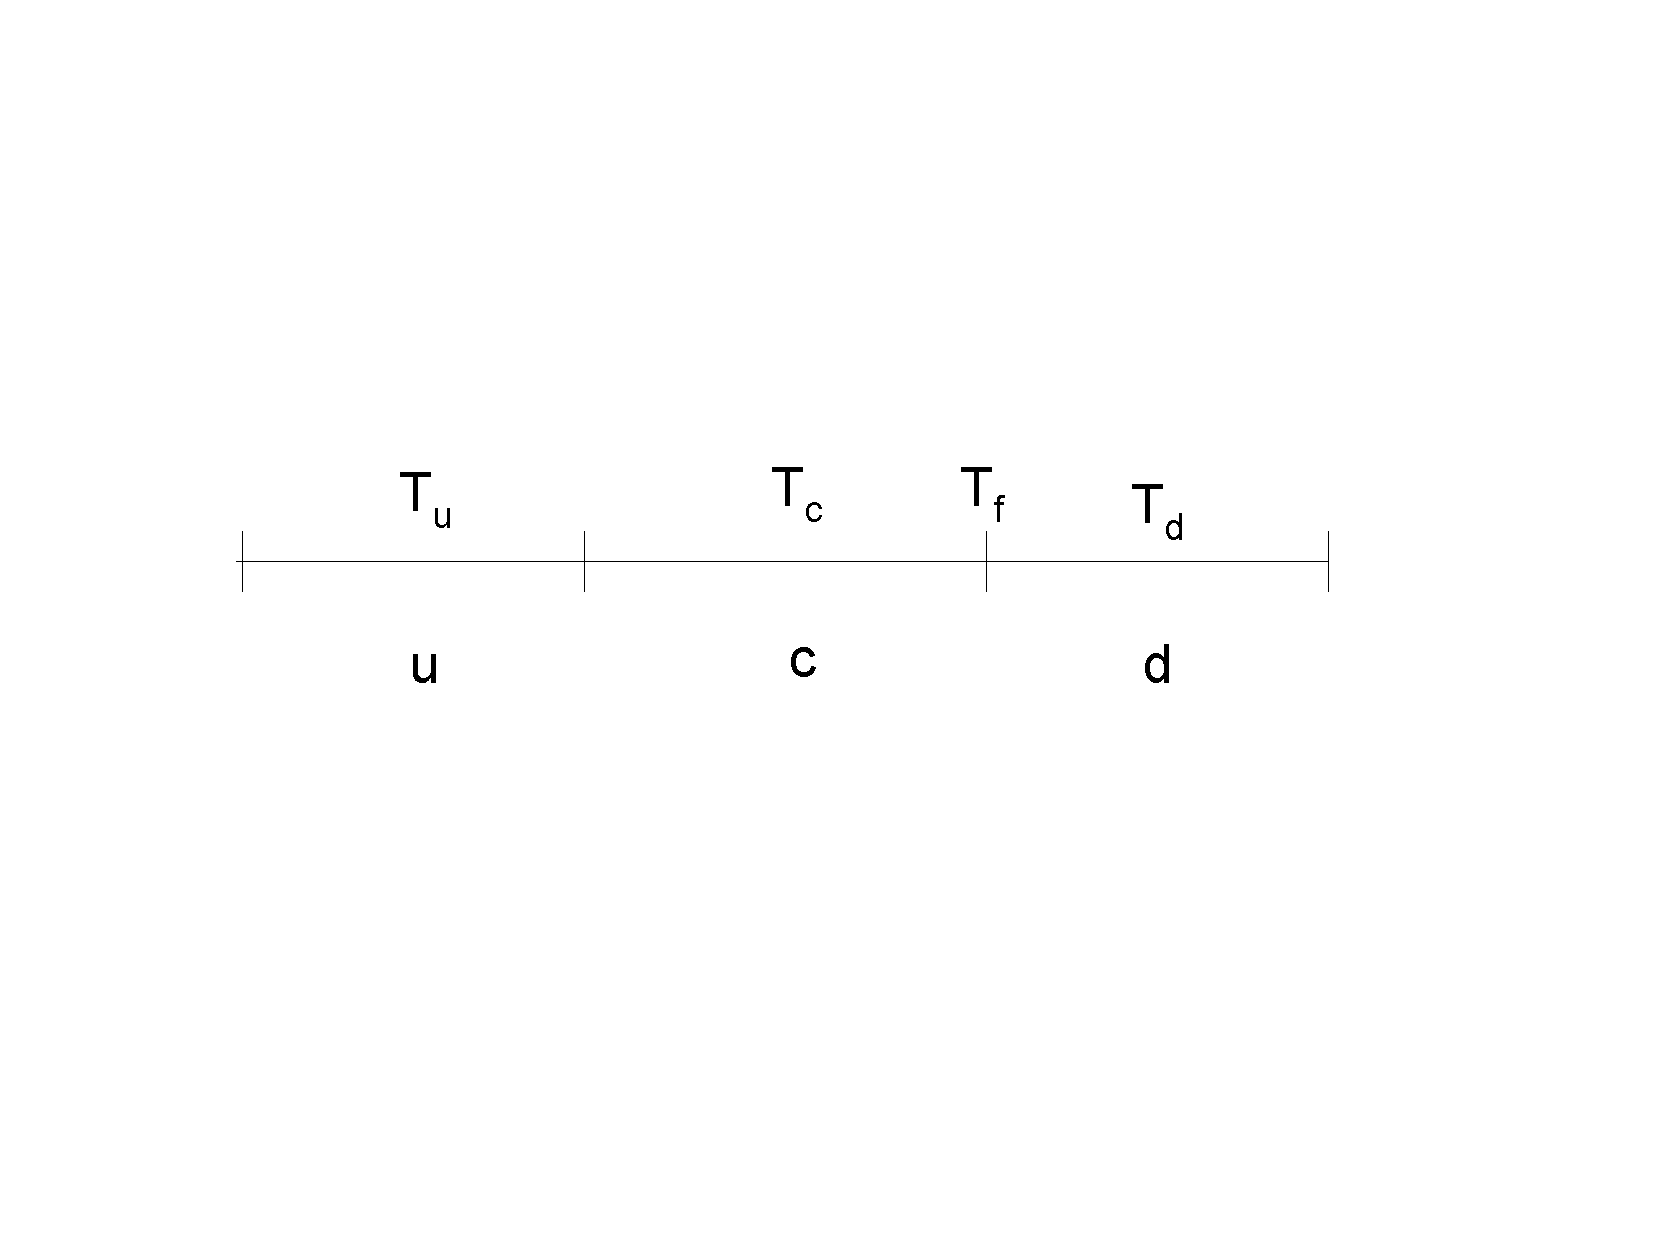
\includegraphics[width=15.0cm,height=10.cm]{./figures/1D_FEM_CV}
\end{center}
\vspace{-5cm}}
\caption{1-D finite element showing CV's {\it u, c, d} and face {\it f}.}
\label{fem_cv_represent_a}
\end{figure}

%%%==============================================
%%% FIGURE 01 - Discretization 
%%%==============================================
\begin{figure}[H]
\vbox{
\begin{center}
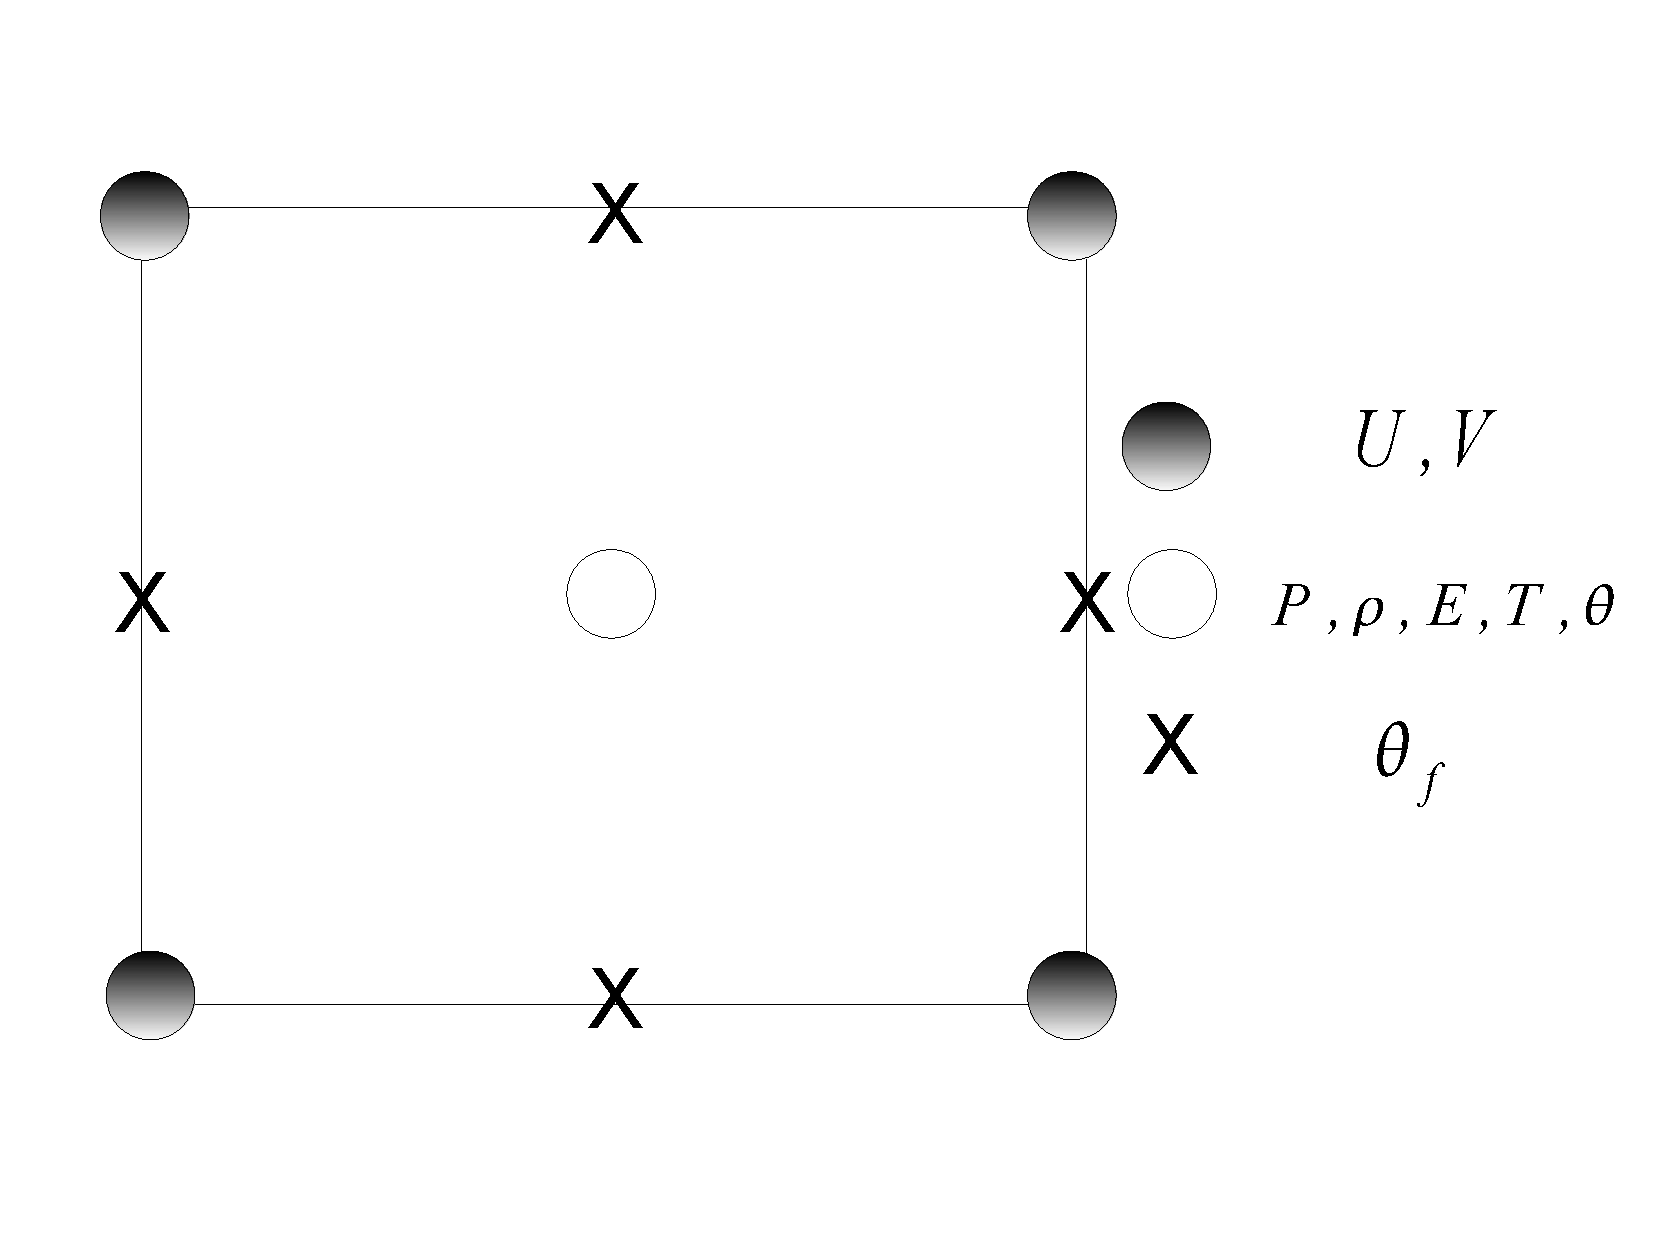
\includegraphics[width=9.0cm,height=7.0cm]{./figures/FEM_elem}
\end{center}
\vspace{-1cm}}
\caption{Finite element used to discretize the fluids equations.  The central position of key solution variables are indicated here.}
\label{fem_cv_represent_b}
\end{figure}

Suppose that each element $i$ of our finite element mesh has a control volume and a solution variable $\hat T_i$ associated with it. Then the FEM solution $\widehat{T}$ is related to the CV solution \textit{T} by
%%
%% - begin displaymath
%%
\begin{displaymath}
\int_{V} N_{i} (\widehat{T} - T) \,d V = 0, \quad
\forall i\in \{1,2,...,{\mathcal N}\}
\end{displaymath}
in which $N_{i}$ is the finite element basis function associated with node \textit{i} and $M_{i}$ is the finite volume basis function (top hat function), which in our formulation is unity over element $i$ and zero elsewhere. In addition, the FEM representation of \textit{T} is given by $\widehat{T} = \sum\limits_{j=1}^{\mathcal{N}} N_{j} \widehat{T}_{j}$. Thus,
%%
%% - begin equation
%%
\begin{equation}
B \underline{\widehat{T}} = Q \underline{T}
\label{BQ}
\end{equation}
with $B = \int\limits_{V} N_{i} N_{j} \,d V$ and $Q =\int\limits_{V} N_{i} M_{j} \,d V$. The vectors $\underline{\widehat{T}} = \left(\widehat{T}_{1}, \widehat{T}_{2}, \ldots, \widehat{T}_{\mathcal{N}} \right)^{T}$, $\underline{T} =\left(T_{1}, T_{2}, \ldots,  T_\mathcal{M} \right)^{T}$ contain the unknown finite element and CV values of $T$, respectively. Both matrices \textit{B} and \textit{Q} have sparse structure.

%%
%%********************************************************
%%********************************************************
%%

\subsection{Extrema detecting}

To determine where to apply first order instead of high order fluxes, extremas must be detected and if there is a smooth transition between the high and low order fluxes, the closeness to an extrema must be quantified. This is achieved using the normal variable diagram NVD approach \index{\fluidity Module! Transport methods! NVD approach} as follows. Suppose $T_{u}, T_{c}, T_{d}$ are ordered consecutively and $T_{f}$ is the face value between CV's \textit{c} and \textit{d} (see Fig. \ref{fem_cv_represent_a}). In which case for a monotonic solution
%%
%% - begin equation
%%
\begin{equation}
\mathcal{T}_{f} = \frac{T_{f} - T_{u}}{T_{d} - T_{u}}  \in [0,1]
\label{p4a}
\end{equation}
where $\mathcal{T}_{f}$ is the non-dimensional high order face value.  The non-dimensional upwind face value is
\begin{equation}
\mathcal{T}_{c} = \frac{T_{c} - T_{u}}{T_{d} - T_{u}}
\label{p4b}
\end{equation}
The idea is to obtain a linear combination $\widetilde{\mathcal{T}}_{f}$ of $\mathcal{T}_{f}$ and $\mathcal{T}_{c}$ such that $\widetilde{\mathcal{T}}_{f}$ equals $\mathcal{T}_{c}$ when there is a local extrema ($\mathcal{T}_{c} \notin [0,1]$ and the scheme becomes first order) and $\widetilde{\mathcal{T}}_{f}$ moves smoothly between this and the high order flux $\mathcal{T}_{f}$ according to the curve shown on the NVD diagram \citep[see][]{gomes_2008}. $\widetilde{T}_{f}$ is calculated from
\begin{equation}
\widetilde{\mathcal{T}}_{f} = \frac{\widetilde{T}_{f} - T_{u}}{T_{d} - T_{u}}.
\label{2.1a}
\end{equation}
The flux limited solution is
\begin{equation}
\widetilde{T}_{f} = \widetilde{\mathcal{T}}_{f} (T_{d} - T_{u}) + T_{u}.
\label{2.1b}
\end{equation}
$\widetilde{\mathcal{T}}_{f}$ (see Fig. \ref{fem_cv_represent_a}) in this equation is calculated from:% (see Fig. \ref{nvddiag}):
\begin{equation}
\widetilde{\mathcal{T}}_{f} =
  \begin{cases}
    \min \{ \widetilde{\gamma} {\cal T}_{c}, \max \{ 0, {\cal T}_f\} \}, & \text{if} \
    \mathcal{T}_{c} \in (0,1); \\
    \mathcal{T}_{f},  & \text{otherwise},
  \end{cases}
\label{2.1c}
\end{equation}
with $\widetilde{\gamma} = 2.0$. Thus at an extrema the first order non-oscillatory method will be applied.  The curve $\mathcal{T}_{f} = 2\mathcal{T}_{c}$ has been chosen as an upper bound on $\widetilde{\mathcal{T}}_{f}$ as this corresponds to a TVD condition in 1-D \index{\fluidity Module! Transport methods! TVD condition} with equally spaced cells/elements \citep[see][]{hirsch_1990}.  One can use larger values of the gradient $\widetilde{\gamma}$ but convergence of the resulting non-linear iteration can suffer.  However, a larger gradient can help maintain sharper features in the solution, as reported by \citet{jasak_1999}.  They recommend the use of a gradient of 6 ($\widetilde{\gamma} = 6$, Eqn. \ref{2.1c}), they also recommend that the gradient should not be greater than 10 and not less than 2.  \citet{piperno_1998} explain some useful criteria for constructing limiting functions.  In addition, they use a maximum NVD curve with C$^{1}$ continuity, which is claimed to improve convergence, and use a quotient of gradients as opposed to the quotient of differences used here in Eqns. \ref{p4a}-\ref{2.1a}. 


\subsection{Extrema detection in multi-dimensions and isotropic limiting}

When integrating over a face of a CV in multi-dimensions we denote the cell from which the velocity is coming from as \textit{c} and the cell to which the velocity is pointing to \textit{d} (as in the previous section) with corresponding solution variables of $T_{c}$ and $T_{d}$ and the far field upwind value $T_{u}$. The value of $T_{u}$, for multi-dimensional  problems, is not well defined and thus it is this the the remainder of this section concerns.

The surface integral in Eqn. \ref{a} is calculated by summing the surface integrals over each face of CV \textit{i}. This face surface integral is evaluated using Gaussian quadrature. The values of $\widehat{T}$ at the Gauss points are limited using the NVD approach as described in the previous section, so that no new extrema are introduced into the solution \textit{T}. This is achieved by considering the velocity at the Gauss points on the face of an element. Out of the two CV's sharing this face, the CV from which the velocity is pointing away from is chosen as CV $c$ and the other CV denoted as \text{d}.


The minimum and maximum value of $T$ of the six CV's in 3-D and four CV's in 2-D, sharing a face with (less than this if near a boundary) with CV $c$ and CV \textit{c} itself, which we denote as $T_{\min}$ and $T_{\max}$. A non-dimensional temperature is then obtained at the Gaussisn integration point from the high order temperature $T_{f}$, via Eqn. \ref{2.1b} with the value of $T_{u}$ obtained from
%%
%% - begin equation
%%
\begin{equation}
T_{u} =
\begin{cases}
   T_{\max}, & \text{if} \ T_{d} \leq T_{c}; \\
   T_{\min}, & \text{if} \ T_{d} > T_{c}.
\end{cases}
\label{rr}
\end{equation}

This then allows the flux limiting, Eqns. \ref{2.1a}-\ref{2.1c} to be applied. This approach is the recommended isotropic limiting method.  One can amend $T_{\max}$ and $T_{\min}$ to take into account variable grid resolution using instead:

\begin{equation}
T_u = T_c + \frac{\Delta_{cd}}{\Delta_{uc}} ( T_{\max} - T_c) 
\end{equation}
\noindent
or\\ 
\begin{equation}
T_u = T_c + \frac{\Delta_{cd}}{\Delta_{uc}} ( T_{\min} - T_c) 
\end{equation}
depending on the criteria in Eqn. \ref{rr}. $\Delta_{cd}$ is proportional to the distance between the CV cells $c$ and $d$ and $\Delta_{uc}$ is proportional to the distance between the CV cells $u$ and $c$. For example, $\Delta_{cd} = \frac{1}{2}(V_c + V_d)$ and  $\Delta_{uc} = \frac{1}{2}(V_{max} + V_c)$ or  $\Delta_{uc} = \frac{1}{2}(V_{min} + V_c)$ again  depending on criteria expressed by Eqn. \ref{rr}. $V_{min}$ is the volume of  the cell surrounding CV $c$ that has a minimum value of $T$,  $V_{max}$ is the volume of  the cell surrounding CV $c$ that has a maximum value of $T$, and $V_c$ and $V_d$ are the volumes of cells $c$ and $d$.  The alternative would be to use geometrical distances to define $\Delta_{cd}$ and $\Delta_{uc}$. 

The most relaxed form of limiting is obtained from
\begin{equation}
\mathcal{T}_{f} = \frac{T_{f} - T_{\min}}{T_{\max} - T_{\min}}
\label{r}
\end{equation}
\noindent
and
\begin{equation}
\mathcal{T}_{c} = \frac{T_{c} - T_{\min}}{T_{\max} - T_{\min}}
\label{r_p}
\end{equation}
which results in useful bounded schemes. Moreover the scheme defined by Eqns. \ref{r} and \ref{r_p} introduce less dissipation than other bounded
schemes. These two flux limiting methods will prevent any new extrema from forming, however for a given direction new extrema can form along this direction results in oscillations in the solution. However, by choosing a control volume value in the upwind direction from face $f$ and just upwind from CV $c$ then this problem can be circumvented.


\subsection{Time Discretization} \label{time_discretisation}\index{\fluidity Module! Transport methods ! Time discretisation}
A new time discretization method has been developed based on Crank-Nicholson time stepping.  The Crank-Nicholson method was chosen, because it has the simplicity of a two level time stepping method, is unconditionally stable and second order accurate. However, the use of time steps of the order of the grid Courant number and above can result in numerical oscillations and unphysical solutions. Thus a parameter $\theta$ is introduced, in which $\theta$ = 0.5 corresponds to the Crank-Nicholson time stepping method and $\theta$ = 1.0 backward-Euler.
Then using Eqns. \ref{CV1} and \ref{a} the time stepping for Eqn. \ref{traneq} takes the form:
%%
%% - begin equation
%%
\begin{eqnarray}
\int M_i \left( \frac{T_{i}^{n+1} -T_{i}^{n}}{\Delta t} - s \right) \,dV= \nonumber \\
\int_{\Gamma_{CV_{i}}} \left[\theta\left(\mathbf{a}^{n+1}\cdot \mathbf{n} \widetilde{T}^{n+1}
+\mathbf{n}\cdot k^{n+1}\nabla \widetilde{T}^{n+1}   \right)+\left(1-\theta\right)\left(\mathbf{a}^{n}\cdot \mathbf{n} \widetilde{T}^{n}
+\mathbf{n}\cdot k^{n}\nabla \widetilde{T}^{n}
 \right)  \right]d\Gamma
 \label{theta}
\end{eqnarray}
For each time step a value of $\theta$ is calculated at each CV face based on the satisfaction of a TVD criteria. In 1-D, assuming the flux limiting values of the flux at the $i-{\frac{1}{2}}$ and $i+{\frac{1}{2}}$ boundaries (see Fig. \ref{fem_cv_represent_c}) are $h^{n}_{i-{\frac{1}{2}}}$ and $h^{n}_{i+{\frac{1}{2}}}$ at time level \textit{n},  the time discretization becomes:
%%
%% - begin equation
%%
\begin{equation}
\Delta x_i \left( \frac{T_{i}^{n+1} - T_{i}^{n}}{\Delta t} \right)
= \theta_{i-\frac{1}{2}}^{n+{\frac{1}{2}}} h_{i-\frac{1}{2}}^{n+1}
+(1-\theta_{i-\frac{1}{2}}^{n+{\frac{1}{2}}}) h_{i-\frac{1}{2}}^n
-\theta_{i+\frac{1}{2}}^{n+\frac{1}{2}} h_{i+\frac{1}{2}}^{n+1}
-(1-\theta_{i+\frac{1}{2}}^{n+\frac{1}{2}}) h_{i+\frac{1}{2}}^n
\label{thetareq1}
\end{equation}
with
%%
%% - begin displaymath
%%
\begin{displaymath}
h_{i-\frac{1}{2}}^{n} = a_{i-\frac{1}{2}}^{n}
T_{i-\frac{1}{2}}^{n}
 +k_{i-\frac{1}{2}}^n \frac{\partial
T^n}{\partial x}\left\vert_{i-\frac{1}{2}}\right.
\end{displaymath}

%%%==============================================
%%% FIGURE 01 - Discretization issues
%%%==============================================
\begin{figure}[H]
\vbox{
\begin{center}
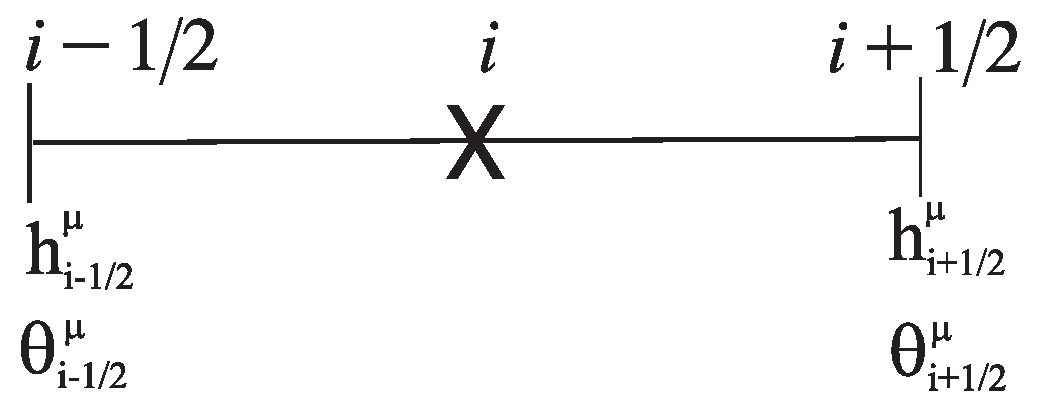
\includegraphics[width=10.0cm,height=7.5cm]{./figures/FEM_elem2}
\end{center}
\vspace{-3.cm}}
\caption{Positioning of variables in and on the boundary of CV {\it i}.}
\label{fem_cv_represent_c}
\end{figure}
%%%==============================================
%%%                 FIGURE 01 
%%%==============================================



%%%==============================================
%%%             FIGURE - P1DGP2
%%%==============================================
\begin{figure}[H]
\vbox{
\hbox{
\hspace{0.cm}
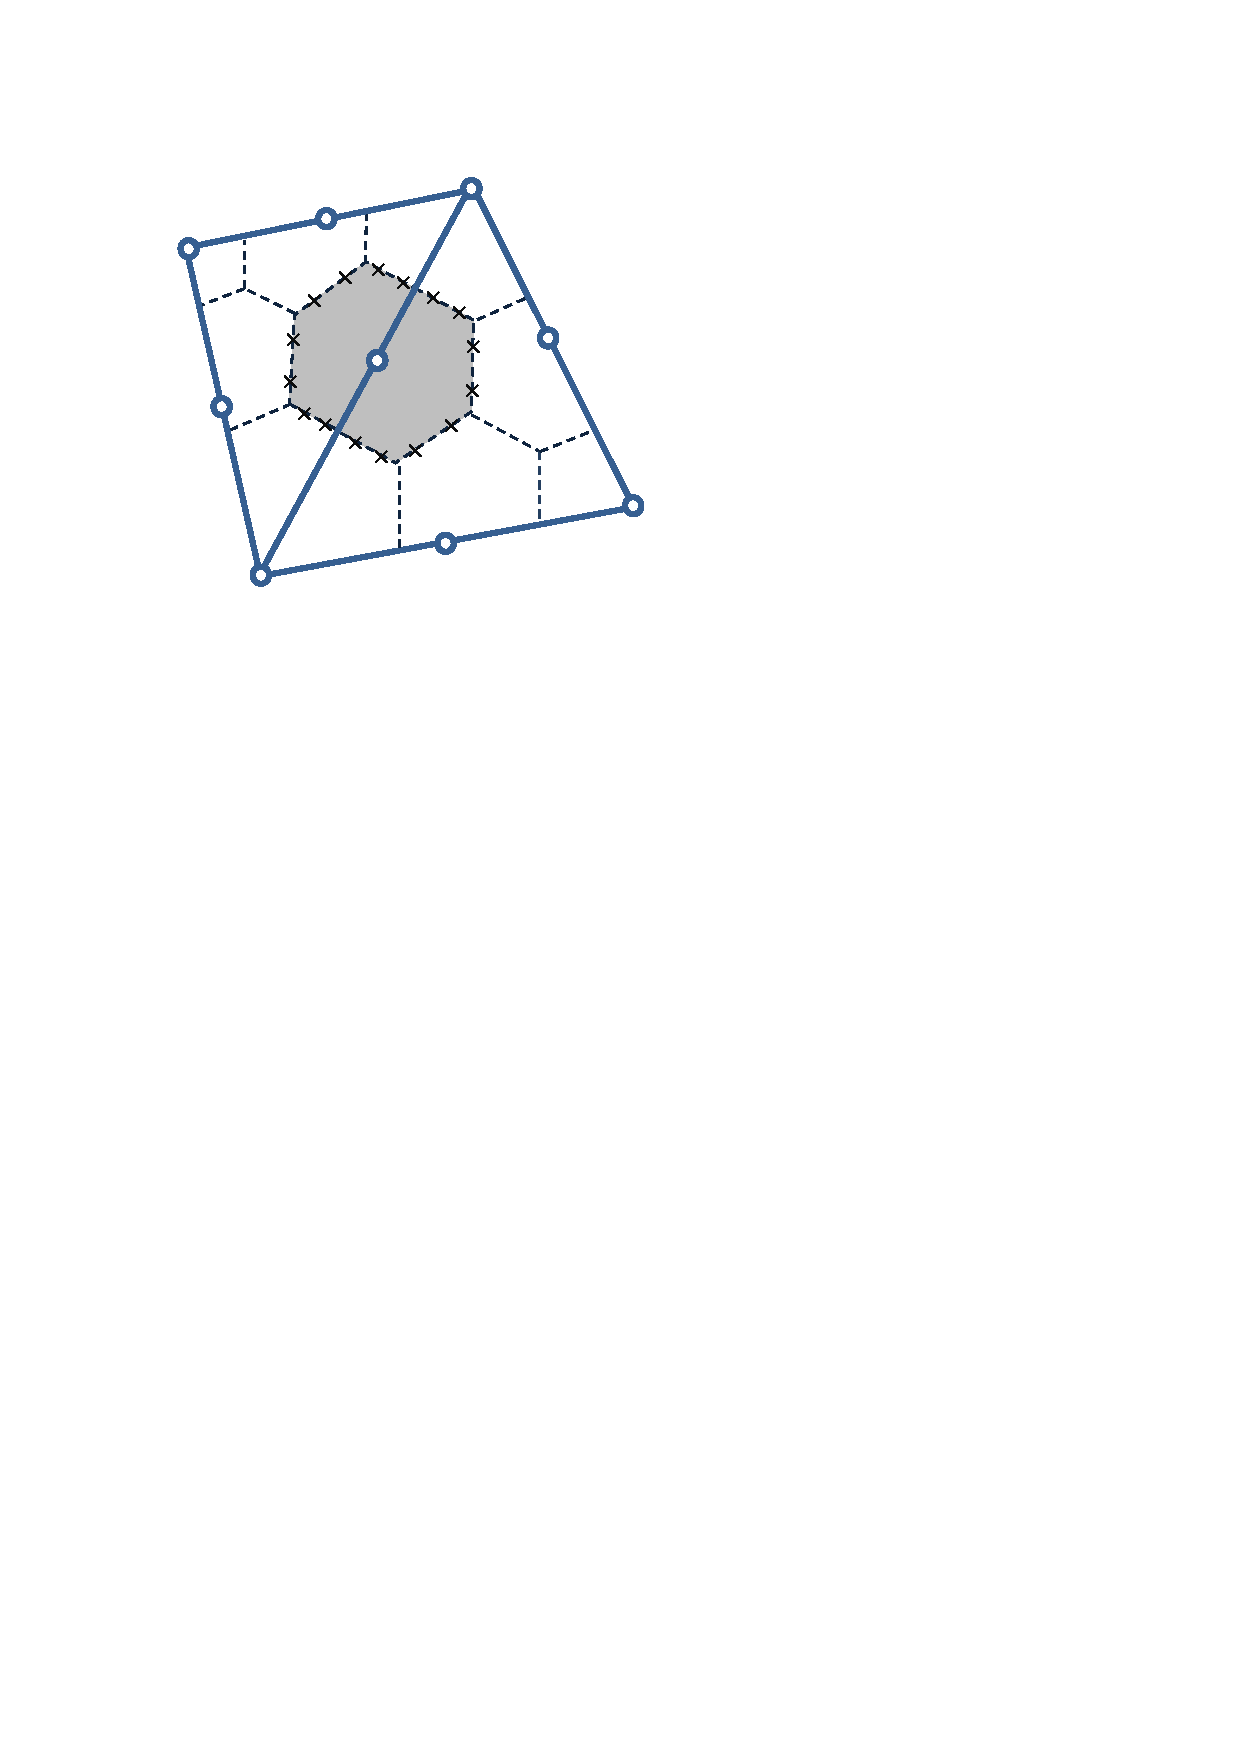
\includegraphics[width=7.0cm,height=7.cm]{./figures/p1dg-p2-elepic}
\hspace{-0.cm}
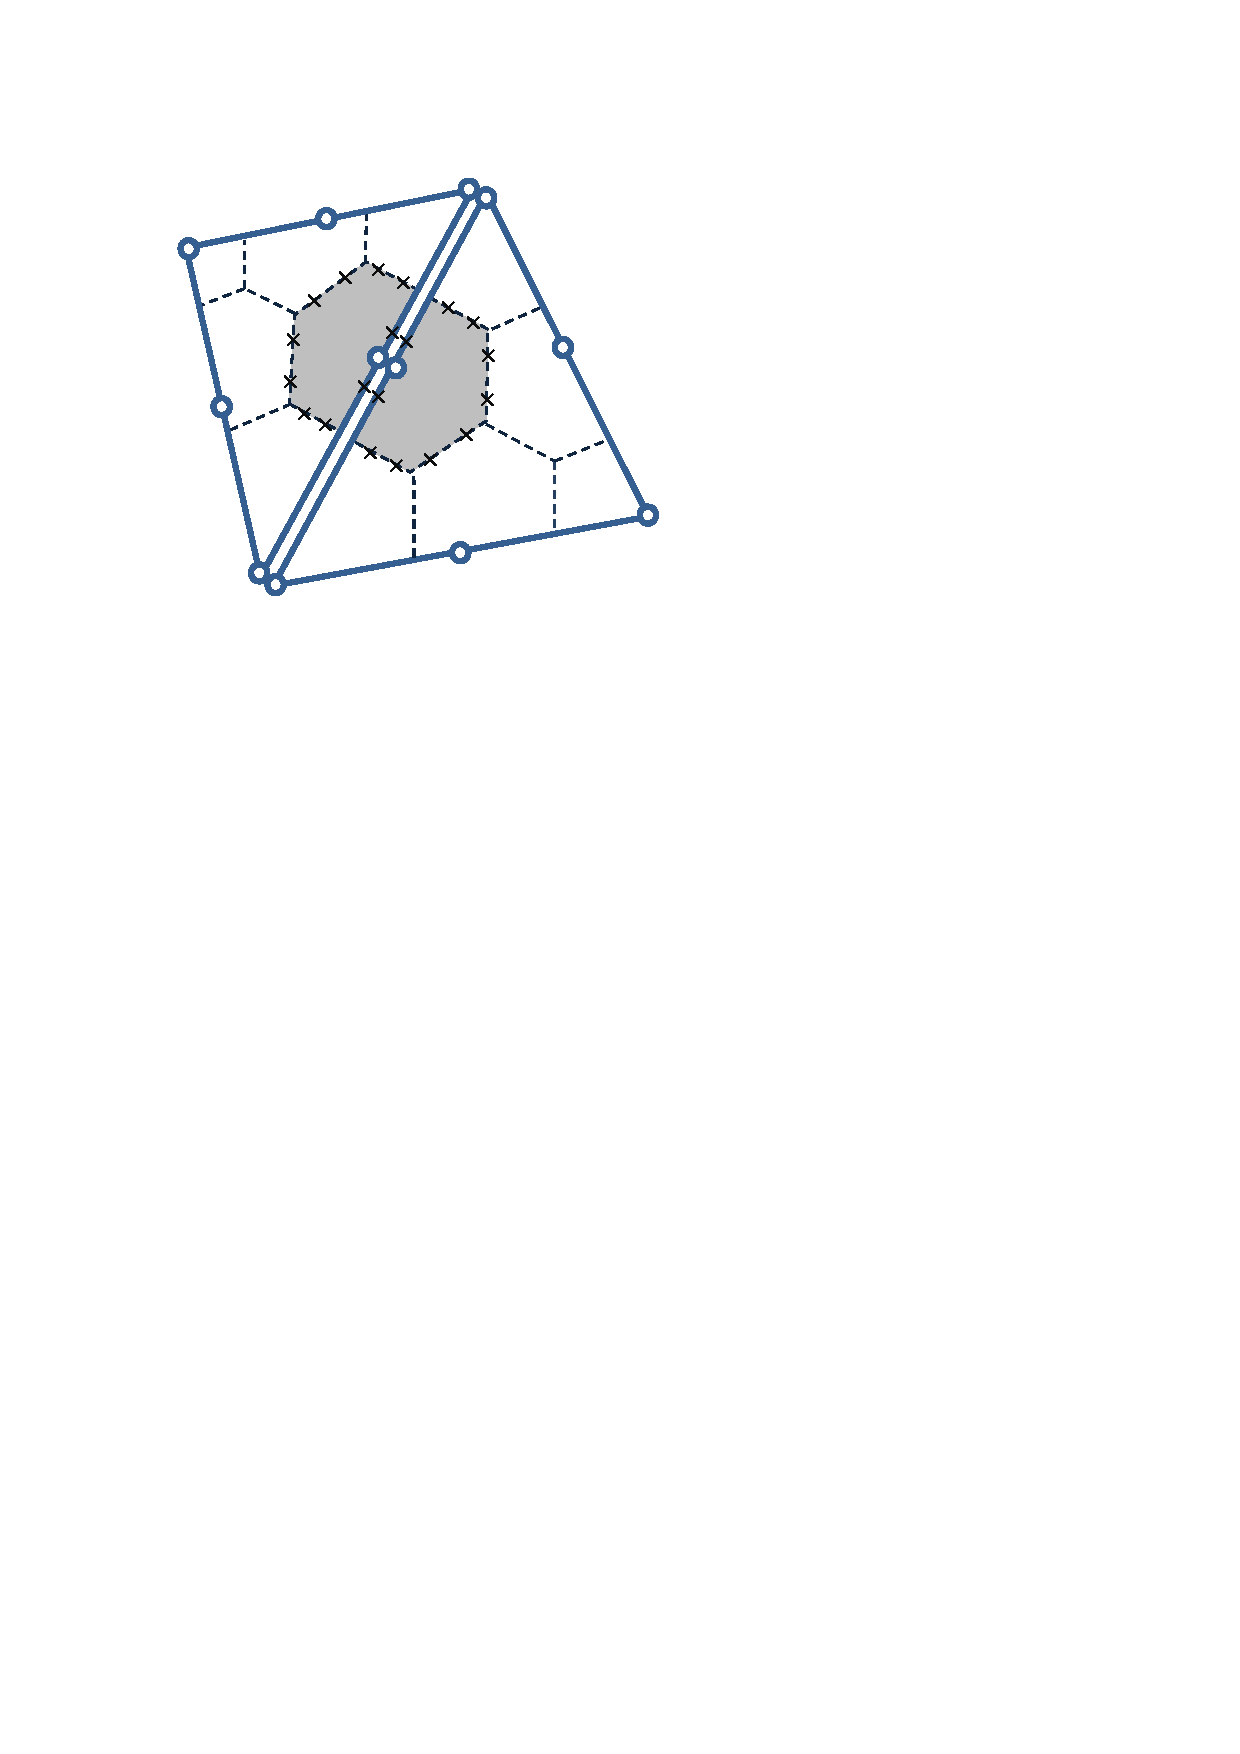
\includegraphics[width=7.0cm,height=7.cm]{./figures/p1dg-p2-dgsat-elepic}
}
\vspace{-0.cm}
\hbox{\hspace{4.cm}(a) \hspace{6.5cm}(b)}
\vspace{-0.cm}}
\label{p1dgp2_ele-dgsat_pics}
\caption{2D finite element containing control volumes is shown. The circles represent the underlying finite element nodes and dashed lines the boundaries of the control volumes. The crosses show typical quadrature points used to integrate around the control volumes. (a) Continuous pressure and tracer solution between the elements. (b) Discontinuous pressure and tracer between elements.  }
\end{figure}
%%%==============================================
%%%             FIGURE - P1DGP2
%%%==============================================

\noindent
$\Delta x_{i}$ is the width of the $i^{th}$ CV and $\theta_{i+\frac{1}{2}}^{n+\frac{1}{2}}$ is the value of $\theta$ associated with face $i+\frac{1}{2}$ and the time step from time level $n$ to $n+1$.  The representation of $k_{i-\frac{1}{2}}^n \frac{\partial T^n}{\partial x}\vert_{i-\frac{1}{2}}$ is considered in a following section.% a simple example of which is $\frac{T_i^{n+1}-T_{i-1}^n}{\Delta x}$ in which $\Delta x$ is the size of the control volumes.  

Re-arranging Eqn. \ref{thetareq1}:
%%
%% - begin displaymath
%%
\begin{eqnarray}
\left( \Delta x_i - \Delta t \frac{\left[
-\widehat{\theta}_{i-\frac{1}{2}}^{n+\frac{1}{2}}(
-h_{i-\frac{1}{2}}^{n+1}+h_{i-\frac{1}{2}}^{n})
+\widehat{\theta}_{i+\frac{1}{2}}^{n+\frac{1}{2}}(
-h_{i+\frac{1}{2}}^{n+1}+h_{i+\frac{1}{2}}^{n}) \right]}
{T_i^{n+1}-T_i^n} \right)
\left(\frac{T_i^{n+1} - T_i^n}{\Delta t} \right) =\nonumber\\
h_{i-\frac{1}{2}}^{n+1}-h_{i+\frac{1}{2}}^{n+1}\nonumber
\end{eqnarray}
with
%%
%% - begin displaymath
%%
\begin{displaymath}
\widehat{\theta}_{i-\frac{1}{2}}^{n+\frac{1}{2}}  = 1-\theta_{i-\frac{1}{2}}^{n+\frac{1}{2}}.
\end{displaymath}
Now since backward Euler time stepping is TVD in the same way that first order upwind scheme is spatially, a positive definite mass matrix is a sufficient condition for the backward Euler scheme above to be TVD \citep[see][]{hirsch_1990}\index{\fluidity Module! Transport methods! TVD condition}.  Thus the diagonal mass matrix (the term in brackets) must be non-negative, after re-arranging this requirement becomes
%%
%% - begin displaymath
%%
\begin{displaymath}
\frac{\Delta t}{\Delta x_{i}\left(T_i^{n+1} - T_i^{n}\right)} \left[ \widehat{\theta}_{i-\frac{1}{2}}^{n+\frac{1}{2}}\left(h_{i-\frac{1}{2}}^{n} - h_{i-\frac{1}{2}}^{n+1}\right)-\hat\theta_{i+\frac{1}{2}}^{n+\frac{1}{2}}\left(h_{i+\frac{1}{2}}^{n}-h_{i+\frac{1}{2}}^{n+1}\right) \right] \leq 1
\end{displaymath}
and thus
%%
%% - begin displaymath
%%
\begin{displaymath}
\left(\widehat{\theta}_{i-\frac{1}{2}}^{n+\frac{1}{2}}
p_{i-\frac{1}{2}}^{n+\frac{1}{2}}
-\widehat{\theta}_{i+\frac{1}{2}}^{n+\frac{1}{2}}
q_{i+\frac{1}{2}}^{n+\frac{1}{2}} \right) \leq 1
\end{displaymath}
with
%%
%% - begin displaymath
%%
\begin{displaymath}
p_{i-\frac{1}{2}}^{n+\frac{1}{2}} = \left( \frac{h_{i-\frac{1}{2}}^{n}
- h_{i-\frac{1}{2}}^{n+1}}{T^{n+1}_{i} - T_{i}^{n}} \right)
\frac{\Delta t}{\Delta x_{i}}  \quad \text{and} \quad
q_{i+\frac{1}{2}}^{n+\frac{1}{2}} = \left(
\frac{h_{i+\frac{1}{2}}^n-h_{i+\frac{1}{2}}^{n+1}}{T^{n+1}_{i} - T_{i}^{n}}
\right) \frac{\Delta t}{\Delta x_{i}}
\end{displaymath}
which is satisfied if
%%
%% - begin equation
%%
\begin{equation}
- \widehat{\theta}_{i-\frac{1}{2}}^{n+\frac{1}{2}}
p_{i-\frac{1}{2}}^{n+\frac{1}{2}} \leq \frac{1}{2} \quad \text{and} \quad
- \widehat{\theta}_{i-\frac{1}{2}}^{n+\frac{1}{2}}
q_{i-\frac{1}{2}}^{n+\frac{1}{2}} \geq
\frac{1}{2}
\label{half}
\end{equation}
Thus to make the value of $\theta_{i-\frac{1}{2}}^{n+\frac{1}{2}}= 1 - \widehat{\theta}_{i-\frac{1}{2}}^{n+\frac{1}{2}}$ as close to $\frac{1}{2}$ as possible we choose
%%
%% - begin displaymath
%%
\begin{displaymath}
\theta_{i-\frac{1}{2}}^{n+\frac{1}{2}} = \max \left\{ \frac{1}{2},
1 - \beta \min \left\{ \left|\frac{1}{p_{i-\frac{1}{2}}^{n+\frac{1}{2}}}\right|,
\left|\frac{1}{q_{i-\frac{1}{2}}^{n+\frac{1}{2}}} \right| \right\} \right\}
\end{displaymath}
with $\beta=\frac{1}{2}$.

\subsection{Multi-dimensional temporal limiting}
\label{multidimtemplim}

The high resolution $\theta$ method can be extended to multi-dimensions by replacing $h_{i-\frac{1}{2}}^{n}$ with the integral of $\tilde{h}_{f}^{n}$ over face \textit{f} and $\Delta x_{i}$ replaced by the volume $L_{i}$ (contribution from diagonal mass matrix) of the $i^{th}$ CV. Using similar arguments to the 1-D case the following expression for $\theta_f^{n+\frac{1}{2}}$ of face \textit{f} is obtained:
%%
%% - begin equation
%%
\begin{equation}
\theta_f^{n+\frac{1}{2}}=\max \left\{ \frac{1}{2}, 1 - \beta \min\left\{
\left|\frac{1}{p_{f}^{n+\frac{1}{2}}}\right|,\left|
\frac{1}{q_{f}^{n+\frac{1}{2}}} \right| \right\} \right\}
\label{thet1}
\end{equation}
with
%%
%% - begin equation
%%
\begin{equation}
p_f^{n+\frac{1}{2}} =
\frac{g_f^{n+\frac{1}{2}}\Delta t}{(T^{n+1}_{c} - T_{c}^{n}) L_{c}}
\quad \text{and} \quad q_f^{n+\frac{1}{2}} =
\frac{g_f^{n+\frac{1}{2}}\Delta t}{(T^{n+1}_{d} - T_{d}^{n}) L_{d}}
\label{thet2}
\end{equation}
and
%%
%% - begin equation
%%
\begin{equation}
g_f^{n+\frac{1}{2}}= (\tilde{h}_{f}^{n} - \tilde{h}_f^{n+1})
\label{gf}
\end{equation}
CV's \textit{c} and \textit{d} in these equations refer to the two CV's that are adjacent to face \textit{f}, (see Fig. \ref{fem_cv_represent_b}). Extensions of this method to differential equations with time-dependent terms like $\frac{\partial \rho T}{\partial t}$ are realized by replacing, in Eqn. \ref{thet2}, $T_j^n$ and $T_j^{n+1}$ by $T_{j}^{n} \rho_{j}^{n}$ and $T_{j}^{n+1} \rho_j^{n+1}$ respectively for $j = c$ and $j = d$.


\subsection{Control Volume Diffusion Discretization}\label{section_diff_discretisation}\index{\fluidity ! Transport methods ! Diffusion discretisation}

The high resolution $\theta$ method can also be used with diffusion by adding to $g_{f}^{n+\frac{1}{2}}$ in Eqn. \ref{gf} the flux limited discretized contribution, integrated along face $i-\frac{1}{2}$.
In 1-D this might lead to
%%
%% - begin displaymath
%%
\begin{displaymath}
g_{i-\frac{1}{2}}^{n+\frac{1}{2}} = h_{i-\frac{1}{2}}^n-h_{i-\frac{1}{2}}^{n+1}
= a_{i-\frac{1}{2}}^n T_{i-\frac{1}{2}}^n -
a_{i-\frac{1}{2}}^{n+1} T_{i-\frac{1}{2}}^{n+1} + \kappa \left(
\frac{T_{i}^n-T_{i-1}^n}{\frac{1}{2}(\Delta x_{i-1}+\Delta x_i )}
- \frac{T_{i}^{n+1}-T_{i-1}^{n+1}}{\frac{1}{2}(\Delta
x_{i-1}+\Delta x_i )}\right)
\end{displaymath}
in which $\kappa$ is the diffusion coefficient. In multi-dimensions this becomes
%%
%% - begin displaymath
%%
\begin{displaymath}
g_{f}^{n+\frac{1}{2}} = \tilde h_{f}^n-\tilde h_{f}^{n+1}
\end{displaymath}
in which
%%
%% - begin displaymath
%%
\begin{equation}
\tilde{h}_{f}^{n} = \int_{\Gamma_f} \left( a \cdot n T^{n}
+ \kappa \frac{\partial T^n}{\partial n_x} \right) \,d\Gamma
\label{16a}
\end{equation}
where $n_x$ is the normal to the control volume. Now if the underlying scheme that calculates $\frac{\partial T^n}{\partial n_x}$ is non-oscillatory then the advection-diffusion scheme will be non-oscillatory. A simple example of this is
%%
%% - begin displaymath
%%
\begin{displaymath}
\frac{\partial T^n}{\partial n_x}\Big\vert_{no_f} = \frac{\partial T^n}{\partial n_x} \Big\vert_{f} = \frac{T_{c}^{n} - T_{d}^{n}}{\Delta x_{f}}
\end{displaymath}
in which, as before, the subscripts denote cells that share face \textit{f} (see Fig. \ref{fem_cv_represent_b}), $\Delta x_{f}$ is a measure of the component of distance between the centres of the CV's \textit{c} and \textit{d} in the normal direction to face $f$. This equation also serves as a definition of $\frac{\partial T^{n}}{\partial n_x}\vert_{no_f}$. The accuracy of this approximation can be improved, but once again non-linearity must be used to ensure boundedness of the scheme. Suppose the underlying non-oscillatory approximation to $\frac{\partial T}{\partial n_x}$ is $\frac{\partial T^n}{\partial n_x}\vert_{no_f}$ then any positive multiple of this will result in a bounded scheme and as such the TVD condition is
%%
%% - begin displaymath
%%
\begin{displaymath}
{\frac{\partial \widetilde{T}^{n}}{\partial n_x}\Big\vert_{f}
\frac{\partial T^{n}}{\partial n_x}\Big\vert_{no_f}} \geq 0
\end{displaymath}
The scheme is bounded if the high order limited derivative $\frac{\partial \widetilde{T}^{n}}{\partial n_x}\vert_{f}$ has the same sign as $\frac{\partial T^{n}}{\partial n_x}\vert_{no_f}$. However, to avoid difficulties with the non-linear convergence the derivative of $\frac{\partial \widetilde{T}^{n}}{\partial n_x}\vert_{f}$ from the high order approximation $\frac{\partial T^{n}}{\partial n_x}\vert_{f}$ is limited with
%%
%% - begin displaymath
%%
\begin{displaymath}
s_f \frac{\partial \widetilde{T}^{n}}{\partial n_x}\Big\vert_f
= \max \left\{ \gamma_2 s_f \frac{\partial T^{n}}{\partial n_x}\Big\vert_{no_f},
\min \left\{ s_f \frac{\partial T^{n}}{\partial n_x}\Big\vert_{f},
\gamma_{1} s_{f} \frac{\partial T^{n}}{\partial n_x}\Big\vert_{no_f} \right\}
\right\}
\end{displaymath}
with
%%
%% - begin displaymath
%%
\begin{displaymath}
\gamma_1 \geq 1 \geq \gamma_2 \geq 0
\end{displaymath}
and
%%
%% - begin displaymath
%%
\begin{displaymath}
s_f =
  \begin{cases}
     1 & \ \text{if} \ \frac{\partial T^n}{\partial n_x}\vert_{no_f} \geq 0; \\
    -1 & \ \text{otherwise} \
\end{cases}
\end{displaymath}
and $\frac{\partial T^{n}}{\partial n_x}\vert_{f}$ is the high order flux, which as with the advection scheme can be obtained from any high order representation of \textit{T}. The authors recommended that  $\gamma_{1} = 2, \ \ \gamma_2 = \frac{1}{2}$.  An example, using the FEM discretization would be to use the derivative along a face $f$ of a control volume from the FEM representation. For derivatives along the boundaries of an element one would use a finite element average of the derivative of the FEM representation of one element and the other sharing this face. 

In the case of a diffusion tensors ${\underline{\underline k}}$ this approach using the approximation: 

\begin{equation}
n\cdot {\underline{\underline k}} \nabla T = 
\min\left\{ \beta_{max}\frc{k_{norm}}{{\Delta x}_{f}} , \max\left\{ \beta_{min}\frc{k_{norm}}{{\Delta x}_{f}} , \left( \frc{k}{\Delta x} \right)_{\text{eff}} \right\} \right\}\left(T_{current}-T_{neighbour}\right)
\label{non-lin-diff}
\end{equation}
where 
%\help
\begin{equation}
\left( \frc{k}{\Delta x} \right)_{\text{eff}} =  
- \frc{1}{2} \frc{ n\cdot \left[ \left({\underline{\underline k}} \nabla T\right)_{neighbour} + \left({\underline{\underline k}} \nabla T\right)_{current} \right] }{T_{current}-T_{neighbour}} 
\label{non-lin-diff-eff} 
\end{equation}
and where $T_{current}$ is the solution in the current control volume and $T_{neighbour}$ is the solution in the neighbouring control volume between which the surface integral around the current control volume is being performed. $k_{norm}$ is the normal component of the tensor ${\underline{\underline k}}$ (normal to the boundary of the control volume) and is approximated here with $k_{norm} =\vert n_x \vert k_{xx}  + \vert n_y \vert k_{yy}+\vert n_z \vert k_{zz}$.  ${\Delta x}_f$ is the distance between the centre of the control volumes associated with $T_{current}$ and $T_{neighbour}$.  $\beta_{min}$ is the minimum fraction of the $\frac{k_{norm}}{{\Delta x}_{f}}$ to use $\left(\right.$we use $\beta_{min}=0.05\left.\right)$ and $\beta_{min}$ defines the upper bound on the value of the effective diffusivity $\left(\right.$we use $\beta_{max}=100\left.\right)$.  Without $\beta_{max}$ as $T_{current}$ and $T_{neighbour}$ become close this would make  $n\cdot {\underline{\underline k}} \nabla T$ large. 

There are three main advantages of the non-linear diffusion scheme above: 
\begin{enumerate}[1)]
\item the method does not introduce oscillations due to the high order representation of diffusion; 
\item the method is high order accurate most of the time; 
\item the method always result in a symmetric positive definite discretisation matrix (a property not shared with many high order diffusion control volume discretisations); 
\item the method results in a compact stencil and thus the resulting matricies are sparse. 
\end{enumerate}

Finally, it is noted that the FEM discretization using linear triangle, tetrahedra, rectangles or hexahedra of the diffusion term can also be bounded with restrictions on the distortion of the elements \citep[see][]{mizukami_1985}.


%%%==============================================
%%% FIGURE 01 - Discretization 
%%%==============================================
\begin{figure}[H]
\vbox{
\begin{center}
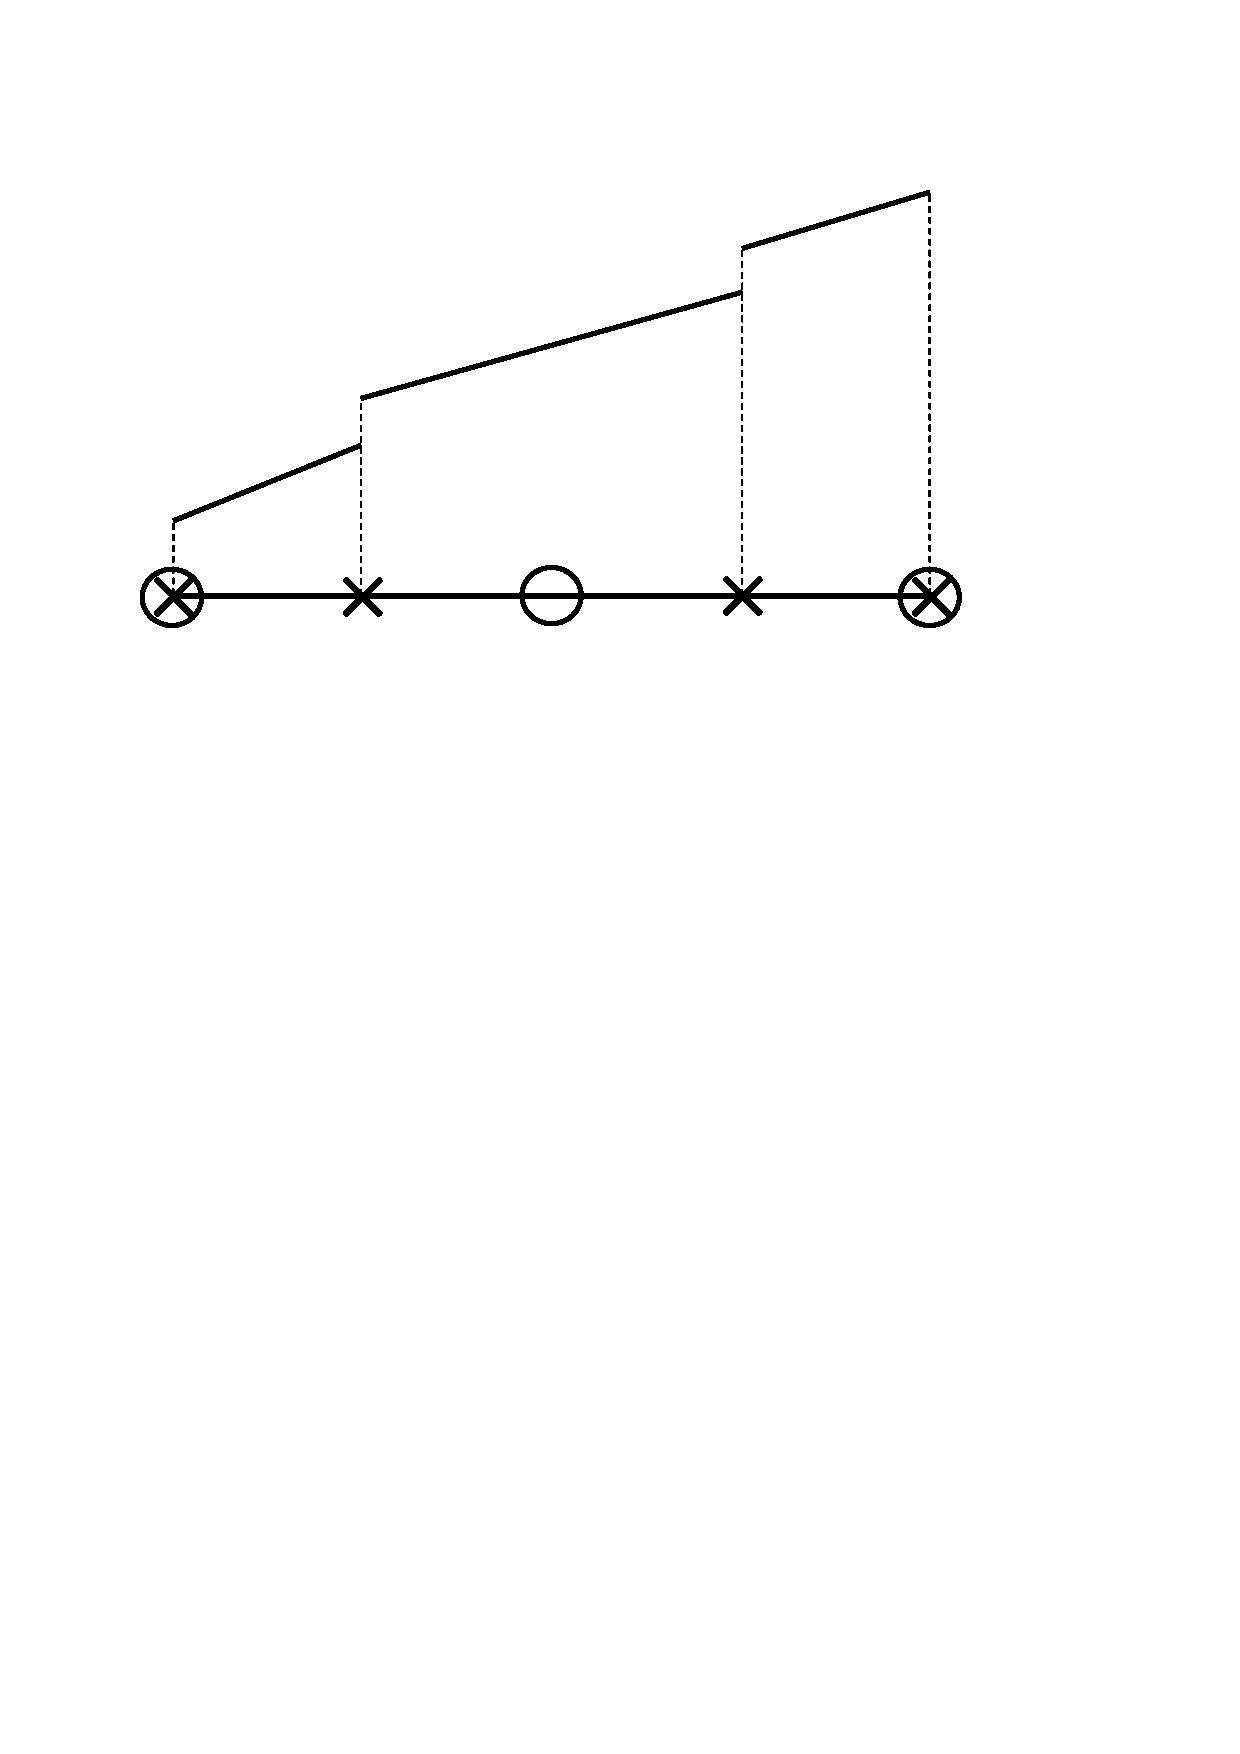
\includegraphics[width=15.0cm,height=10.cm]{./figures/CVFEM_1D}
\end{center}
\vspace{-1cm}
}
\caption{1-D finite element }
\label{fem_cv_represent_c}
\end{figure}

\subsection{Discontinuous Galerkin diffusion discretisation}

A simple form the DG discretised equations for diffusion is: 

\begin{equation}
\int_{V_{ele}} \nabla Q_i {\underline {\underline k}} \nabla T_{fem}^n d\Omega 
+\int_{\Gamma_{ele}} Q_i \alpha \left({T_{fem}^n}_{current}-{T_{fem}^n}_{neighbour} \right)  d\Gamma . 
\label{dg-variational-diff-low} 
\end{equation}
This has an underlying variational principle behind it. That is 
\begin{equation}
\frac{1}{2}
\int_{V_{ele}} \nabla T_{fem}^n {\underline {\underline k}} \nabla T_{fem}^n d\Omega 
+\frac{1}{2} 
\int_{\Gamma_{ele}} \alpha \left({{T_{fem}^n}_{current}-{T_{fem}^n}_{neighbour}} \right)^2 
d\Gamma, 
\label{variational-prin} 
\end{equation}
 and 
thus the discretised equations are guaranteed to be symmetric and positive definite as long as ${\underline {\underline k}}$ is sym-pos-def and scalar $\alpha$ is positive. The first term in Eqn. \ref{variational-prin} attempts to flatter the solution within an element and the latter surface integral attempts to produce continuity of the solution between elements. This is very similar to the way Robin boundary condition are typically applied using FEM: 
%%
%% - begin displaymath
%%
\begin{displaymath}
k \frac{\partial T^{n}}{\partial n} = \alpha (T - T_{0})
\end{displaymath}
can be applied directly in Eqn. \ref{16a}.

Testing with DG basis function $Q_i$ and applying Greens theory to the diffusion term one obtains: 

\begin{equation}
\int_{V_{ele}} \nabla Q_i \underline {\underline k} \nabla T_{fem}^n d\Omega 
-\int_{\Gamma_{ele}} Q_i n\cdot \underline {\underline k} \nabla T_{fem}^n d\Gamma . 
\label{dg-variational-diff-high} 
\end{equation}
If one can turn this into the same form as Eqn. \ref{dg-variational-diff-low} (with a suitable chosen $\alpha$) then the stencil will be very compact and the method of evaluating the diffusion term for DG will have the same advantages as for CV as listed in Section \ref{section_diff_discretisation}.  The first term in Eqn. \ref{dg-variational-diff-high} is formed simply by placing  $T_{fem}^n=\sum_j Q_j {T_{fem}^n}_j$ into this equation. However, the term $n\cdot \underline {\underline k} \nabla T_{fem}^n $ is approximated as described in the next section from derivatives both sides of the element interface. That is the diffusion operator between elements is formed in the same manner as for the control volume discretisation using:
\begin{equation}
\left( \frac{k}{\Delta x} \right)_{eff} =  
- \frac{1}{2} \frac{ n\cdot \left[\left({\underline{\underline k}} \nabla T_{fem}\right)_{neighbour} + \left({\underline{\underline k}} \nabla T_{fem}\right)_{current} \right] }{{T_{fem}}_{current}-{T_{fem}}_{neighbour}} . 
\label{dg-non-lin-diff-eff} 
\end{equation}
This is bounded from above and below using an equation similar to Eqn. \ref{non-lin-diff}, but with a length scale $\Delta x_f$ being the distance between the centroids of the neighbouring elements. Therefore:
\begin{equation}
\alpha=\min\left\{  \beta_{max}\frac{k_{norm}}{{\Delta x}_{f}} , \max\left\{ \beta_{min}\frac{k_{norm}}{{\Delta x}_{f}} , 
\left( \frac{k}{\Delta x} \right)_{eff}
\right\} \right\} 
\label{dg-alpha-def} 
\end{equation} 
and is a positive scaler. 
 


\subsection{Finite element interpolation of the control volume solution} 
To obtain the finite element solution $T_{fem}^n$ we use a Galerkin projection of $T_{fem}^n$ onto the control volume solution $T^n$. This is tested with the finite element basis functions $N_i$. $N_i$ is discontinuous between elements only when $T$ is. Thus when there is no discontinuity of solution between all elements then a global mass matrix system needs to be solved:
 \begin{displaymath}
 \int_V N_i (T_{fem}^n- T^n) d\Omega =0, 
\end{displaymath}
to form the high order solution $T_{fem}^n$.  


\subsection{Calculating the high order derivatives}

In order to obtain the high order derivatives used in the calculation of the limited diffusion term, Eqn. \ref{non-lin-diff-eff}, the finite element solution within each element is used along with boundary conditions from the finite element solution of the surrounding elements or the boundary conditions on the domain, if the elements are next to the domain boundaries. 
That is $\frac{\partial T^n}{\partial x}$ is calculated from
 \begin{equation}
 B {\underline T_{fem}^n}_x = \underline v_x^n, \;\;
 B {\underline T_{fem}^n}_y = \underline v_y^n, \;\;
 B {\underline T_{fem}^n}_z = \underline v_z^n, 
\label{form-derivs}
\end{equation}
with $B_{ij}=\int Q_i Q_j dV$, ${T_{fem}}_x=\sum_j Q_j {{T_{fem}}_x}_j$ and is discontinuous as the basis functions $Q_i$ are discontinuous between elements. In addition,
 \begin{eqnarray}
&& \underline v_x^n=\int Q_{i} \frac{\partial T_{fem}^n}{\partial x} d\Omega 
-\int_{\Gamma_{ele}} n_x Q_i ({T_{fem}^n}_{current}-{T_{fem}^n}_{nab})d\Gamma, \nonumber \\
%\end{equation}
% \begin{equation}
&& \underline v_y^n=\int Q_{i} \frac{\partial T_{fem}^n}{\partial y} d\Omega 
-\int_{\Gamma_{ele}} n_y Q_i ({T_{fem}^n}_{current}-{T_{fem}^n}_{nab})d\Gamma, \nonumber \\
%\end{equation}
 %\begin{equation}
&& \underline v_z^n=\int Q_{i} \frac{\partial T_{fem}^n}{\partial z} d\Omega 
-\int_{\Gamma_{ele}} n_z Q_i ({T_{fem}^n}_{current}-{T_{fem}^n}_{nab})d\Gamma. 
\end{eqnarray}
Dirichlet boundary conditions are applied through the surface integral around each element ${\Gamma_{ele}}$.  

The values of the derivatives either side of the control volume face are placed into Eqn. \ref{non-lin-diff-eff}. These may be the same value for example within an element or when there is continuity of solution $T^n$ or $T_{fem}^n$ between elements. The same approach is also used to form the diffusion operator for DG based on equation \ref{}.  The solution of equations \ref{form-derivs} are local to each element as 
the matrix is a Discontinuous Galerkin mass matrix $B$ and 
thus does not couple the elements. 




\subsection{Time limiting for the non-conservative advection equation}

The transport term is often expressed in non-conservative form. Due to the fact that the equations for inviscid single phase flow are not necessarily well posed, solving the internal energy equation in non-conservative form is often a recourse.  One can obtain imaginary eigenvalues when the problem is posed as a Riemann problem and thus the solutions tend to diverge exponentially. A common solution is to solve for conservative variables e.g.$\rho$, $\rho\mathbf{a}$, $\rho T$ or to use a non-conservative form of the internal energy equation. This has the form 
%%
%% - begin equation 34
%%
\begin{equation}
\rho \left( \frac{\partial T}{\partial t} + \mathbf{a}\cdot\nabla
T \right) + \nabla \cdot \kappa\nabla T  = S
\end{equation}
or in the more general multi-phase form is:
%%
%% - begin equation 35
%%
\begin{equation}
{C_p}_k \alpha_k \rho_k \left( \frac{\partial T_k}{\partial t} + \mathbf{a}_k\cdot\nabla
T_k \right) + \nabla \cdot \kappa_k \nabla T_k  = S_k
\label{multiT}
\end{equation}
in which $k$ is the fluid phase, ${C_p}_k$ the specific heat capacity at constant pressure, $\alpha_k$ is the volume fraction of phase $k$, $T_k$ is the temperature of phase $k$, $S_k$ the energy source or sink and $\mathbf{a}_k$ is the velocity of phase $k$. To solve this equation it is divided by the heat capacity ${C_p}_k$.

Integrating this equation over the $i^{th}$ CV, using
%%
%% - begin equation 36
%%

\begin{eqnarray}
\alpha_k \rho_k
\mathbf{a}_k \cdot \nabla T_k = \nabla \cdot \alpha_k\rho_k \mathbf{a}_k T_k - T_k\nabla\cdot \alpha_k \rho_k \mathbf{a}_k
\label{parts}
\end{eqnarray}
and applying the divergence theorem to the spatial derivative to obtain

%%
%% - begin equation 37
%%
\begin{eqnarray}
&&\int M_{i} {\alpha_k}_i^{n+1} {\rho_k}_{i}^{n+1} \left(
\frac{{T_k}_{i}^{n+1}-{T_k}_{i}^{n}}{\Delta t} \right)  dV +
\nonumber\\
&&\int_{\Gamma_{CV_{i}}} \left(\theta^{n+\frac{1}{2}} \left[
\mathbf{a}^{n+1}_k \cdot \mathbf{n} {\widetilde{\alpha}}_k^{n+1}
{\widetilde{\rho}}_k^{n+1} (\widetilde{T_k}^{n+1}-{T_k}_i^{n+1})
+\kappa_k \mathbf{n}\cdot \nabla T^{n+1}_k \right]\right. +\nonumber\\
&&\left.(1-\theta^{n+\frac{1}{2}} )\left[ \mathbf{a}^{n}_k \cdot
\mathbf{n} {\widetilde{\alpha}}_k^{n} {\widetilde{\rho}}_k^{n}
(\widetilde{T}^{n}_k-{T_k}_i^{n}) +\kappa_k \mathbf{n}\cdot \nabla
T^{n}_k \right]\right)\nonumber\\
&&d\Gamma = \int M_{i} s_k^{n+\frac{1}{2}}/{C_p}_k dV
\label{nocons}
\end{eqnarray}


With a value of $\theta^{n+\frac{1}{2}}={\frac{1}{2}}$ the above scheme is second order accurate in time. However, in order for the scheme to be non-oscillatory $\theta_{f}^{n+\frac{1}{2}}$ will be defined as explained in Section \ref{multidimtemplim}, with $\tilde{h}^{n}_{f}$ defined by
%%
%% - begin equation 38
%%

\begin{equation}
\tilde{h}^{n}_{f}=\int_{\Gamma_{f}}
\left(\mathbf{a}_k\cdot \mathbf{n}\alpha_k \rho_k \widetilde{T}^{n}_k
+\kappa_k \mathbf{n}\cdot \nabla  T^{n}_k  \right)d\Gamma
\end{equation}
Here the terms involving $T_i^{n+1}$ and $T_i^n$ in Eqn. \ref{nocons} have not been included in the derivation of the value of $\theta$. They have not been included here in an attempt to achieve consistency with the multi-phase thermal energy equation in conservative form. If they are included then the values of $\theta_f^{n+\frac{1}{2}}$ on the CV faces (used in Eqn. \ref{nocons}) can be easily derived based on the derivation in the previous section.

The variables $\alpha_k$, $\rho_k$ and $T_k$ are spatially limited individually as explained in the previous section to obtain a scheme that is bounded in all these variables. In addition, on the boundaries of the domain appropriate boundary conditions (e.g. specified values resulting from incoming fluid) for each of these variables are required and are placed in the surface integrals of Eqn. \ref{nocons} on the boundary of the domain.


\subsection{Time discretisation of multi-phase reaction terms}
A coupled set of multi-phase flow equations containing the exchanges between the phases is of the form: 
\begin{equation}
D \frac{\partial \Psi}{\partial t} + H \Psi = s_\psi. 
\label{w-rho-e-prob}
\end{equation}
For positive diagonal matrix $D$. Using $\hat \Psi = D^{-\frac{1}{2}} \Psi$ and $\hat H=D^{-\frac{1}{2}} H D^{-\frac{1}{2}}$ then this equation becomes: 

\begin{equation}
\frac{\partial \hat \Psi}{\partial t} + \hat H \hat \Psi = \hat s_\psi
\label{w-rho-e-prob}
\end{equation} 
with 
\begin{equation}
\hat H
= L \Lambda R. 
\label{stab_matrix}
\end{equation}
which is the eigen-value decomposition into matrices of left $L$ and right $R$ eigen vectors and diagonal matrix of eigen-values $\Lambda$. Typically if there are no losses then (e.g. conservation of mass) then $\hat H$ is a discrete Laplacian. Thus we obtain the diagonal system: 
\begin{equation}
\frac{\partial \hat {\hat \Psi}}{\partial t} + \Lambda \hat{\hat\Psi} = \hat{\hat s}_\psi
\label{e-prob}
\end{equation} 
with $\hat\Psi=R\Psi$ the solution will grow (ignoring other losses) if any of the eigen-values in $\Lambda$ are negative. In general their values will be non-negative (based on the physics and conservation) and $H$ sym-pos-semi-definite.  Thus this can be treated as a set of independent equations and an optimal values for the contributions in the diagonal matrix $\Theta$ chosen. So the time discretisation becomes:


\begin{equation}
\frac{\hat {\hat \Psi}^{n+1}-\hat {\hat \Psi}^{n}}{\Delta t} + \Lambda \Theta\hat{\hat\Psi}^{n+1} +\Lambda(I-\Theta) \hat{\hat\Psi}^n= \hat{\hat s}_\psi
\label{e-prob-time-term-opt-theta}
\end{equation} 
which becomes on mapping to original variables: 

\begin{equation}
D\frac{ { \Psi^{n+1}}- {\Psi^{n}}}{\Delta t} 
+ D^{\frac{1}{2}} L\Lambda \Theta R D^{\frac{1}{2}} {\Psi^{n+1}}
+ D^{\frac{1}{2}} L\Lambda (I-\Theta) R D^{\frac{1}{2}} {\Psi^{n}} 
= \hat{\hat s}_\psi
\label{e-prob-time-term-opt-theta-orig-var}
\end{equation} 

Now considering just one variable. That is any one of 
the equations in equation set \ref{e-prob} takes on the form: 

%%
%% - begin equation
%%
\begin{equation}
\displaystyle\frac{\partial {T}\left({r},t\right)} {\partial t}+{\sigma}\left(t\right){T}\left({r},t\right)={s}\left({r},t\right)
\label{eqn57}
\end{equation}
Discretising Eqn. \ref{eqn57} in time using the $\theta$-time stepping method yields:
\begin{eqnarray}
&&\left(\displaystyle\frac{{{T}}^{n+1}\left({r},t\right)-{{T}}^{n}\left({r},t\right)}{\Delta t}\right)+{\theta}^{n+\frac{1}{2}}\left({r}\right){\sigma}^{n+\frac{1}{2}}\left(t\right){{T}}^{n+1}\left({r}\right)+   \nonumber \\
&& \left({I}-{\theta}\left({r},t\right)\right){\sigma}^{n+\frac{1}{2}}\left(t\right){{T}}^{n}\left({r},t\right)=  {\theta}^{n+\frac{1}{2}}\left({r}\right){s}^{n+1}\left({r}\right)+\left[{I}-{\theta}^{n+\frac{1}{2}}\left({r}\right)\right]{s}^{n}\left({r}\right)
\label{eqn60}
\end{eqnarray}
Now suppose ${s}\left({r}\right)$ is spatially and time invariant then we can match our numerical solution with the analytical solution by choosing and appropriate matrix ${\theta}^{n+\frac{1}{2}}\left({r}\right)$; the diagonal values of this matrix are
\begin{eqnarray}
{\theta}^{n+\frac{1}{2}}\left({r}\right) = \max \left\{ 
0.5,
\left(\displaystyle\frac
{{\sigma}^{n+\frac{1}{2}}\left(t,n+\frac{1}{2}\right)\Delta t-1.0+\exp\left(-\Delta{\sigma}^{n+\frac{1}{2}}\left(t,n+\frac{1}{2}\right)\right)} 
{{\sigma}^{n+\frac{1}{2}}\left(t,n+\frac{1}{2}\right)\Delta t\left(1.0-\exp\left(-\Delta t{\sigma}^{n+\frac{1}{2}}\left(t,n+\frac{1}{2}\right) \right)\right) }
\right)
\right\}. 
\label{eqn61}
\end{eqnarray} 
However, if the most important attribute of the scheme is that it achieves physical realism then it is appropriate to use the TVD criteria for ${\theta}\left({r}\right)$, which is
%%
%% - begin equation 62
%%
\begin{equation}
{\theta}^{n+\frac{1}{2}} \left({r}\right) \geq 1-\displaystyle\frac{1}{\Delta t {\sigma}^{n+\frac{1}{2}}\left({r}\right)}
\label{eqn62}
\end{equation}
This criteria is easily derived by ensuring that the scheme is a positive multiple of the backward Euler scheme.  In fact, Eqn. \ref{eqn61} for $\theta^{n+\frac{1}{2}}$ tends to this expression from below, thus $\theta^{n+\frac{1}{2}}$, given by Eqn.\ref{eqn61} satisfies the TVD criteria.

This expression has assumed that the material properties have been evaluated at time level ${n+{\frac{1}{2}}}$ and are thus constant through out the time step. This method of time discretisating 
involving material properties has been used elsewhere \cite{ChrisNSE}.




\subsection{Mass conservation and volume fraction advection}\index{\fluidity Module! Transport methods ! Volume fraction advection} 

The multi-phase continuity equation is
\begin{eqnarray}
\frac{\partial \rho_k\alpha_k}{\partial t}
+ \nabla \cdot \mathbf{a}_k \rho_k \alpha_k = {S_c}_k
\label{cty}
\end{eqnarray}

and the corresponding discretized continuity equation becomes

\begin{eqnarray}
&&\int M_{i}  \left( {\rho_k}_{i}^{n}
\left(\displaystyle\frac{{\alpha_k}_{i}^{n+1}-{\alpha_k}_{i}^{n}}{\Delta
t}\right) + {\alpha_k}_{i}^{n}
\left(\displaystyle\frac{{\rho_k}_{i}^{n+1}-{\rho_k}_{i}^{n}}{\Delta
t}\right) \right)dV + \nonumber\\
&&\int_{\Gamma_{CV_{i}}}\left( \theta^{n+\frac{1}{2}}
 \mathbf{a}^{n+1}_k \cdot \mathbf{n}\widetilde{\alpha}_k^{n+1} \widetilde{\rho}_k^{n+1}
\widetilde{\alpha}^{n+1}_k
+
(1-\theta^{n+\frac{1}{2}} )
 \mathbf{a}^{n}_k \cdot \mathbf{n}\widetilde{\alpha}_k^{n} \widetilde{\rho}_k^{n}
\widetilde{\alpha}^{n}_k
  \right) d\Gamma
=
\int M_{i} {{s_c}_k}^{n+\frac{1}{2}} dV
\label{disc-cty}
\end{eqnarray}
in which ${{s_c}_k}^{n+\frac{1}{2}}$ is the mass source/sink for fluid phase $k$. To enhance stability it is beneficial to treat the term involving ${\rho_k}_i^{n+1}$ implicitly in pressure (this allows the CFL condition associated with acoustic waves to be exceeded) and this is absorbed into the discretized equation for pressure \citep[see][for more details]{pain_2001b}.  The continuity equation, Eqn. \ref{cty} and discretized continuity equation, Eqn. (\ref{disc-cty}), are embedded in the energy Eqns. \ref{multiT} and \ref{nocons} respectively.

\subsection{Solving the Linear Equations}\index{\fluidity Module! Transport methods ! Linear solvers}

One of the main advantages of the finite element high resolution method (HRFEM) that it shares with most other FEM methods, is that the equations involve diagonal dominant mass matrixes which are well conditioned and have a condition number independent of the grid size.

In contrast to first order discretization methods, the HRFEM equations have coupling in all directions. The HRFEM method used here is obtained by making each element a CV and using a mapping between the CV and the FEM solution. The FEM solution is then used as the high order flux along the CV faces. The HRFEM method requires the inverse of the consistent mass matrix in order to calculate incoming control volume fluxes accurately - this inverse is a full matrix. Thus this coupling in practice can only be realized explicitly in the iterative scheme.  The HRFEM method has been generalised with a bi-jective mapping between the FEM and CV solutions. The discontinuous HRFEM method also uses consistent mass matrices, but these are local to an element so they are more manageable and can be treated implicitly.

There are a number of options available for solving the non-linear HRFEM equations. One can linearize the global equation set, treating implicitly or explicitly the down stream element coupling (inclusion of down stream coupling may result in poorer conditioned matrices from the discretization). Then a global set of linear equations would be solved each non-linear iteration by for example using SSOR preconditioning for GMRES \citep{saad_1986}.  Alternatively, one can sweep through each CV, resolving all the non-linear equations local to each CV with a suitable liberalization procedure.

The global or local to an element liberalization can be achieved using the Newton-Raphson method, although this has quadratic convergence properties it is prone to failure when there does not exist a good initial guess. The most robust method reported for other flux limiting methods is to linearize on the first-order equations \citep[see][]{darwish_1993}.  This involves solving a matrix equation with a matrix obtained from the underlying first order spatial discretization and the deviation of the high order scheme from this, would be treated explicitly as a source term. This has the advantage that the resulting matrix is well conditioned and also the non-linear convergence to a solution is usually monotonic, due to the dissipative characteristics of the first order scheme and is thus the approach adapted here.


\section{Discretisation of Force Balance Equation} 


\subsection{Continuous Pressure Formulation} 

The force balance equation is:
\begin{equation}
{\underline {\underline \sigma}}_k {\mathbf u}_k = - \nabla p + {\mathbf s}_u, 
\label{force-bal}
\end{equation}
with boundary conditions of either
${{\mathbf u}_k}\cdot {\mathbf n} = {{ u}_k}_{bc}$ (applied through the continuity or saturation equation below) or $p = p_{bc}$. 

The basic force balance equation is obtained by using the discontinuous basis function ${\mathbf Q}_i$ for velocity and $M_i$ for pressure and in which in 3D ${\mathbf Q}_i$ becomes:
\begin{equation}
{\mathbf Q}_i = 
  \begin{pmatrix}
    Q_i   & 0 & 0 \\
    0   & Q_i & 0 \\
    0 & 0 & Q_i
  \end{pmatrix}
\label{m_sigma_matrix}
\end{equation}

 Thus the discretete force balance becomes:

\begin{equation}
\int_\Omega {\mathbf Q}_i ({\underline {\underline \sigma}}_k {\mathbf u}_k - \nabla p -{\mathbf s}_u) dV 
+  \int_{\Gamma_{\Omega}} {\mathbf Q}_i {\mathbf n} (p - p_{bc}) d\Gamma =0
\label{force-semi-disc}
\end{equation}
where ${\mathbf n}$ is the normal to the surface 
and $\Omega$ is the domain of solution and 
${\Gamma_{\Omega}}$ the surface of the domain, ${\mathbf s}_u$ is 
the source and the velocity ${\mathbf u}_k = \phi {\mathbf v}_k$, 
$\phi$ is the 
element-wise 
porosity and ${\mathbf v}_k$ is the interstitial fluid velocity of phase $k$. 

Since $p$ is continuous between elements this becomes:

\begin{equation}
{\mathbf M}_\sigma \underline {\mathbf u} = {\mathbf C} \underline {\bf p} 
+ \underline {\bf s}_u. 
\label{force-balance-matrix-form}
\end{equation}
The pressure vector is $\underline{\bf p} =(p_1\; p_2 \; p_3\; ...\; p_{\cal M})^T$, 
the velocity vector is decomposed into phases, thus for two phases, 
$\underline{\mathbf u}=(\underline{\mathbf u}_1^T \;\; \underline{\mathbf u}_2^T)^T$ 
and $\underline{\mathbf u}_k=({{\mathbf u}_k}_1\; {{\mathbf u}_k}_2\; {{\mathbf u}_k}_3\; ...\; {{\mathbf u}_k}_{\cal Q}) $ 
and ${\mathbf u}_k = \sum_{j=1}^{\cal Q} {\mathbf Q}_j{{\mathbf u}_k}_j$ and 
$p=\sum_{j=1}^{\cal M} M_j{p}_j$. Also 


\begin{equation}
{{\mathbf M}_\sigma}^{kk}_{ij} =  \int_\Omega {\mathbf Q}_i 
{\underline {\underline \sigma}}_k {\mathbf Q}_j dV, 
\end{equation}
and for two phase flow

\begin{equation}
{{\mathbf M}_\sigma} = 
  \begin{pmatrix}
    {{\mathbf M}_\sigma}^{11}   & 0 \\
    0   & {{\mathbf M}_\sigma}^{22} 
  \end{pmatrix}
\label{m_sigma_matrix}
\end{equation}
and 

\begin{equation}
{\mathbf C}_{ij}=\int_\Omega {\mathbf Q}_i \nabla M_j dV 
+ \int_\Gamma \frac{1}{2}{\mathbf Q}_i {\mathbf n}  M_j d\Gamma,
\end{equation} 
and 

\begin{equation}
{{\bf s}_u}_i= \int_\Omega {\mathbf Q}_i {\mathbf s}_u dV 
- \int_\Gamma \frac{1}{2}{\mathbf Q}_i {\mathbf n} p_{bc} d\Gamma. 
\end{equation}
where ${\mathbf n}$ is the surface normal. 

Thus as usual with mixed formulations not specifying a 
boundary condition for pressure corresponds to a no 
normal flow conditions which is realized through the continuity 
equation and a weakly applied Dirichlet no normal 
flow boundary condition. 



\subsection{Discretisation of force balance - discontinuous pressure formulation} 

The only difference between this formulations (as far as the force balance 
is concerned) and the continuous formulation is the treatment of pressure 
which is discontinuous along with saturation and density at element 
boundaries. The descret force balance becomes:
\begin{equation}
\int_{\Omega_E} {\mathbf Q}_i ( {\underline {\underline \sigma}}_k 
{\mathbf u}_k - \nabla p -{\mathbf s}_u) dV 
+  \int_{\Gamma_{E}} \frac{1}{2}{\mathbf Q}_i {\mathbf n} (p - p_{nab}) d\Gamma 
+  \int_{\Gamma_{E}-\Gamma} {\mathbf Q}_i {\mathbf n} (p - p_{bc}) d\Gamma =0
\end{equation}
and thus: 

\begin{equation}
{\mathbf C}_{ij}=\int_{\Omega_E} {\mathbf Q}_i \nabla M_j dV 
+ \int_{\Gamma_{E}-\Gamma} \frac{1}{2}{\mathbf Q}_i {\mathbf n} M_j d\Gamma 
+ \int_\Gamma {\mathbf Q}_i {\mathbf n} M_j d\Gamma .
\end{equation}
This corresponds to a central difference discretisation for pressure 
on the boundaries of each finite element, that is for example:

\begin{equation}
\int_{\Omega_E} {\mathbf Q}_i \nabla p dV = -\int_{\Omega_E} \nabla {\mathbf Q}_i  p dV 
+ \int_{\Gamma_E} {\mathbf Q}_i {\mathbf n} p_{nab} dV 
= \int_{\Omega_E} {\mathbf Q}_i \nabla p dV 
+ \frac{1}{2} \int_{\Gamma_E} {\mathbf Q}_i {\mathbf n} (p-p_{nab}) dV
\label{dg-sat-form}
\end{equation}
where $p_{nab}$ is the pressure from the neighboring 
element and ${\mathbf n}$ is the surface normal. 


\subsection{The overlapping finite element method for multi-phase Darcy Flow} 

So far for uniform ${\underline{\underline \sigma}}_k$ within each element and the use of the P1DG-P2 element type 
and its equivalent in 1D the Darcy flow equation is 
exactly enforced. Although this is not true of the DG variants 
for pressure it is observed that it is close 
as the pressure does not have large discontinuities 
between elements at least in one dimension. 

However, ${\underline{\underline \sigma_k}}$ depends on the saturation $S_k$ which has 
a control volume (CV) distribution and is a non-linear function of $S_k$. 
Thus 			

\begin{equation}
{\underline {\underline \sigma}}_k 
= \frac{1}{{Rel}_k} {\underline{\underline K}}^{-1} 	
\end{equation}
in which the permeability tensor 
${\underline{\underline K}}$ has an element wise variation 
and ${Rel}_k$ is the relative permeability. 
Thus in general ${\underline {\underline \sigma}}_k$ varies between elements and within each element 
depending on the same variation as the CV saturation $S_k$ that is $Rel_k$. 
Thus ${\underline {\underline \sigma}}_k$ is piecewise constant 
within each element and a natural 
way to obtain an exact solution would be to use basis functions 
local to each CV within each element. 
Thus if for quadratic pressure variation there will be 
a piecewise 
linear velocity field with simple discontinuity between 
elements and one could then use linear basis functions 
and test functions within each control volume. Thus in 1D 
there would be $2\times 3$ velocity nodal values associated with 
each phase.  

However, such an approach is cumbersome especially in multi-dimensions. 
In fact it may become inpracticle. To overcome this 
problem overlapping basis functions are used. The approach is derived 
based on the observation 
that the only difference between the velocities 
within each CV is a multiplication factor 
and this multiplication factor is ${\underline {\underline \sigma}}_k^{-1}$. 
Thus one can discretise  
using: 
\begin{equation}
\int_\Omega {\mathbf Q}_i^\mu ({\underline{\underline\sigma}}_k^\mu {\mathbf u}_k^\mu - \nabla p -s^\mu) dV + 
\int_{\Gamma}\gamma {\mathbf Q}_i^\mu {\mathbf n} (p-p_{bc}) d\Gamma =0 
\label{overlap-eqn} 
\end{equation}
in which ${\mathbf Q}_i^\mu$ are the weighting functions. 
${\mathbf Q}_i^\mu$ are also the  
velocity basis functions which span the whole 
element that they belong too and also ${\mathbf Q}_i^\mu={\mathbf Q}_i^1\;\; \forall \mu\in\{1,2,...,{\cal N}_{locCV}\}$
where ${\cal N}_{locCV}$ is the number of local control volumes within each 
finite element and ${\mathbf u}_k =\sum_\mu \sum_j H^\mu {{\mathbf u}_k}_j^\mu$ where 
$H^\mu=1$ in local control volume $o$ and $=0$ otherwise. 
It also enables relatively low order quadrature rules to be used 
across each finite element.  
For 2D quadatric pressure triangular elements (see figure \ref{p1dgp2_ele-dgsat_pics}) 
there are $3\times6=18$ velocity basis 
functions for each of the two directions and each phase. 
For 3D quadatric pressure 
tetrahedra elements there are $4\times 10=40$ velocity basis 
functions for each of the two directions and each phase.

The result is again the recovery of the exact enforcement of 
the differential equation at least away from the boundaries. 
Now including in the previous formulation $\gamma=1$ however 
we now need to take into account the difference in the 
volumes of the elements as we integrate right 
across the whole element. This is taken into account 
using 

\begin{equation}
\gamma^\mu = \frac{V^\mu_E}{V_E} \frac{S^\mu_E}{S_E}
\label{overlap-eqn-gamma}
\end{equation}
in which $V_E$ is the volume of element $E$ 
and $V^\mu_E$ is the volume of control volume $\mu$ 
in element $E$ and $S_E$ is the surface area of the element 
on the boundary and $S^\mu_E$ is the surface 
area of element $E$ of CV $\mu$ in element $E$ on the boundary 
of the domain. 

The discontinuous formulation is also easily extended 
to this overlapping finite element approach and becomes: 

\begin{equation}
\int_{\Omega_E} \hat{\mathbf Q}_i^\mu ({\underline{\underline{\sigma}}}_k^\mu {\mathbf u}_k^\mu - \nabla p -{\mathbf s}_u^\mu) dV 
+  \frac{1}{2}\int_{\Gamma_{E-\Omega}} \gamma^\mu_E {\mathbf Q}_i^\mu {\mathbf n} (p - p_{nab}) d\Gamma 
+  \int_{\Gamma_{\Omega}}  \gamma^\mu_E \hat{\mathbf Q}_i^\mu {\mathbf n} (p - p_{bc}) d\Gamma =0. 
\label{overlap-eqn-dg}
\end{equation}
and given that 
\begin{equation}
{\mathbf Q}_j=\hat{\mathbf Q}_i^\mu 
\end{equation}
for a suitable index $j$ the discretisation can be expressed 
similar to equation \ref{force-semi-disc} for the continuous formulation and 
equation \ref{dg-sat-form} for the discontinuouse 
between elements pressure/saturation formulation. 



\subsection{Implicit treatment of buoyancy} 
Given that the saturation/density equation for phase 
$k$ (equation \ref{detail-sat-eqn-k}) can be expressed as:

\begin{equation}
 \frac{\phi{S_k}_i^n( {\rho_k}_i^{n+1}-{\rho_k}_i^n)} {\Delta t} ) 
 + {v_z}_k {S_k}_i^n \frac{\partial \tilde \rho_k^n }{ \partial z}  
= {{s_k}_{rest}}_i
\label{sat-part} 
\end{equation}
where $z$ is the vertical direction in which gravity points. 

The force balance equation with gravity is at time level $n+1$: 

\begin{equation}
{\underline {\underline\sigma}}_k^{n+1} {\mathbf u}_k^{n+1} = \nabla p^{n+1} - \rho_k^{n+1} {\mathbf g} 
\end{equation}
in which ${\mathbf g}$ is the gravitational vector with a 
magnitude $\vert{\mathbf g}\vert$ 
equal to the stength of gravity and the direction in which gravity acts. 
Thus this becomes on inserting \ref{sat-part} into this equation 
for $\rho_k$:


\begin{equation}
{\underline {\underline\sigma}}_k^{n+1} {\mathbf u}_k^{n+1} 
+  {{\underline {\underline\sigma}}_k}_{relax} 
({\mathbf u}_k^{n+1} - {\tilde {\mathbf u}}_k^{n+1}) 
= \nabla p^{n+1} 
-
{\tilde \rho}_k^{n+1} {\mathbf g} 
\end{equation}
in which the matrix has a 'vertical' component: 

\begin{equation}
{{\sigma_k}_{relax}}_{zz} = \vert{\mathbf g}\vert  \Delta t 
\frac{1}{ \phi } 
\max\{ \frac{\partial  {\tilde \rho}_k^{n+1}}{\partial z}, 0\} 
\end{equation}
all other components of the matrix ${{\sigma_k}_{relax}}$ are zero. 
In addition the tildes represent the best guess of 
the variables they are associated with. 

This allows much larger time steps to be used in stratified 
flows and also increases accuracy in these environments. 



\subsection{Discretisation of inertia terms using DG} 
Considering a single phase $k$ the inertial 
terms in conservative form are: 

\begin{equation}
\frac{\partial \hat\rho_k u_k}{\partial t} 
+ \nabla \cdot \hat\rho_k \tilde u_k  u_k 
\label{inertia-eqns-cons} 
\end{equation}
and in non-conservative form: 

\begin{equation}
\hat\rho_k \left(\frac{\partial u_k}{\partial t} 
+  \tilde u_k\cdot \nabla u_k \right) 
\label{inertia-eqns-non-cons} 
\end{equation}
in which $\hat\rho_k= \phi S_k \rho_k$ for porous 
media and $\hat\rho_k= \alpha_k \rho_k$ for inertia dominant 
flows. 
Discretising in conservative form this becomes: 


\begin{equation}
\frac{
\int_{V_e} N_i \hat\rho^{n+1} u^{n+1}_k -
\int_{V_e} N_i \hat\rho^{n} u^{n}_k }
{\Delta t} 
- 
\int_{V_e} \nabla N_i 
(\theta \hat\rho_k^{n+1} \cdot \tilde u_k^{n+1} u_k^{n+1} +
(1-\theta) \hat\rho_k^{n} \cdot \tilde u_k^{n} u_k^{n} ) dV 
\label{inertia-disc-cons-1} 
\end{equation}
\begin{equation}
+ 
\int_{\Gamma_e (n\cdot \tilde u_k^{n+1}<0)} 
 N_i \theta ( \hat\rho_k^{n+1} n\cdot \tilde u_k^{n+1}  
u_k^{n+1})_{nab}  d\Gamma 
+ 
\int_{\Gamma_e (n\cdot \tilde u_k^{n}<0)} 
 N_i(1-\theta) (\hat\rho_k^{n} n\cdot \tilde u_k^{n} 
u_k^{n})_{nab}  d\Gamma 
\label{inertia-disc-cons-2} 
\end{equation}
\begin{equation}
+ 
\int_{\Gamma_e (n\cdot \tilde u_k^{n+1}>0)} N_i 
\theta  \hat\rho_k^{n+1} 
n\cdot \tilde u_k^{n+1}    u_k^{n+1}  d\Gamma
+ 
\int_{\Gamma_e (n\cdot \tilde u_k^{n}>0)} N_i 
 (1-\theta) \hat\rho_k^{n} n\cdot \tilde u_k^{n}  u_k^{n} d\Gamma ,
\label{inertia-disc-cons-3} 
\end{equation}
in which $nab$ refers to variables associated 
with neighboring elements and the surface 
$\Gamma_e (n\cdot \tilde u_k^{n+1}<0)$ is 
the incoming surface to 
element $e$ in which 
$n\cdot \tilde u_k^{n+1}<0$. 
In non-conservative form: 


\begin{equation}
\frac{
\int_{V_e} N_i \hat\rho^{n+\theta_\rho} u^{n+1}_k -
\int_{V_e} N_i \hat\rho^{n+\theta_\rho} u^{n}_k }
{\Delta t} 
+ 
\int_{V_e} N_i \hat\rho_k^{n+\theta_\rho}
(\theta  \tilde u_k^{n+1} \cdot\nabla u_k^{n+1} +
(1-\theta)  \tilde u_k^{n} \cdot\nabla u_k^{n} ) dV 
\label{inertia-disc-non-cons-1} 
\end{equation}
\begin{equation}
- 
\int_{\Gamma_e (n\cdot \tilde u_k^{n+1}<0)} 
N_i \theta \hat\rho_k^{n+\theta_\rho} n\cdot \tilde u_k^{n+1} (u_k^{n+1} - (u_k^{n+1})_{nab} ) d\Gamma 
\label{inertia-disc-non-cons-2} 
\end{equation}
\begin{equation}
- 
\int_{\Gamma_e (n\cdot \tilde u_k^{n}<0)} N_i (1-\theta)\hat\rho_k^{n+\theta_\rho} n\cdot \tilde u_k^{n}  (u_k^{n+1} - (u_k^{n+1})_{nab} ) d\Gamma . 
\label{inertia-disc-non-cons-3} 
\end{equation}

										

\section{Discretised saturation equation and global mass balance} 

This section outlines the discrete saturation equations and derives the global mass balance equations from the saturation equations. The resulting equation can then be solved simultaneously with equation \ref{force-balance-matrix-form}. 
										

\subsection{Discretised saturation equation} 

The saturation equation 

\begin{equation}
\phi\frac{\partial \rho_k S_k }{\partial t} 
+ \nabla \cdot {\mathbf u}_k \rho_k S_k = {s_{cty}}_k, 
\end{equation}
discretised by testing it with CV basis functions 
 $M_i$ is and discretising in time using the 
 $\theta-$method is:
 
\begin{equation}
\int_\Omega M_i (\frac{\phi{\rho_k}_i^n ({S_k}_i^{n+1}-{S_k}_i^n) }{\Delta t} 
+ \frac{\phi{S_k}_i^n( {\rho_k}_i^{n+1}-{\rho_k}_i^n)} {\Delta t} ) dV
+ \int_{\Gamma_{CV_i}} {\mathbf n} \cdot {\mathbf u}_k^{n+\theta} \rho_k^{n+\theta} S_k^{n+\theta} 
d\Gamma 
= \int_\Omega M_i {s_{cty}}_k^{n+\theta} dV.
\label{detail-sat-eqn-k}
\end{equation}
 
 
\subsection{Discretised global continuity equation} 
 
Dividing equation \ref{detail-sat-eqn-k} by ${\rho_k}^n_i $ and summing 
over all phases one obtains the global continuity equation: 

 
\begin{equation}
 \sum_k \left(
\int_\Omega M_i (\frac{ \phi({S_k}_i^{n+1}-{S_k}_i^n) }{\Delta t} 
+ \frac{\phi{S_k}_i^n( {\rho_k}_i^{n+1}-{\rho_k}_i^n)} {{\rho_k}_i^n\Delta t} ) dV
+ \frac{1}{{\rho_k}_i^n}\int_{{\Gamma_{CV}}_i} 
{\mathbf n} \cdot {\mathbf u}_k^{n+\theta} \rho_k^{n+\theta}   S_k^{n+\theta} d\Gamma
- \frac{1}{{\rho_k}_i^n} \int_\Omega M_i {s_{cty}}_k^{n+\theta} dV \right) =0,
\label{detail-sat-eqn-k-sum}
\end{equation}

The saturations and densities are flux limited in space and 
time as explained in section \ref{fluid_transport_methods_section}. This uses a finite element 
interpolation of the saturations and densities which are limited. 
			


Using $\sum_{k=1}^{\cal K} {S_k}_i^n =1, \;\; \forall n$ and linear 
$\rho_k^{n+1}$ about the CV pressure variation $P_{CV}^{n+1}$ then 

\begin{equation}
 \sum_k ( \int_{\Omega} M_i 
( \frac{{S_k}_i^n \frac{\partial \tilde{\rho_k}_i^{n+1}}{\partial \tilde{ p_{CV}}_i^{n+1}}({p_{CV}}_i^{n+1}-\tilde{p_{CV}}_i^{n+1})
} {{\rho_k}_i^n\Delta t} 
+ \frac{{S_k}_i^n( \tilde{\rho_k}_i^{n+1}-{\rho_k}_i^n)} 
{{\rho_k}_i^n \Delta t} ) dV
\end{equation}
\begin{equation}
+ \frac{1}{{\rho_k}_i^n}\int_{{\Gamma_{CV}}_i} {\mathbf n} \cdot {\mathbf u}_k^{n+\theta} \rho_k^{n+\theta} S_k^{n+\theta} d\Gamma
- \frac{1}{{\rho_k}_i^n} \int_\Omega M_i {s_{cty}}_k dV ) =0.
\label{detail-global-cty}
\end{equation}
In matrix form this becomes:

\begin{equation}
{\mathbf M}_p \underline{\bf p}^{n+1} + {\mathbf B}^T \underline{\bf u}^{n+1} 
= \underline{\bf s}_p. 
\label{glob-cty-matrix}
\end{equation}

Notice that in equation \ref{detail-global-cty} the 
control volume-wise variation of pressure ${p_{CV}}_i^n$ has been 
used and in order to get to the equation  \ref{glob-cty-matrix} 
above the finite element variation of pressure with basis 
functions $N_i$ has been used. Thus to get to equation 
\ref{glob-cty-matrix} the Galerkin projection

\begin{equation}
\int_{\Omega} M_i (p_{CV}^n-p^n) dV =0
\end{equation}
for $p^n$ is used. This results in solving the matrix 
equation for ${\bf p}^n$: 

\begin{equation}
{\mathbf M}_{CV} \underline{\bf p}_{CV}^n = {\mathbf N}_{CVfem} \underline {\bf p}^n
\end{equation}
in which the matrix ${\mathbf M}_{CV}$ is diagonal and thus 
this can easily help form the matrix ${\mathbf M}_p$ in equation 
\ref{glob-cty-matrix}. 

\subsection{Compressibility - CV and FEM pressure variations}

Having both a CV and FEM variation of pressure allows us to 
simultaneously have an exact representation of the force balance 
equation as well as ensuring robustness of the the scheme 
e.g. positive densities from potentially complex equations 
of state. When using complex EoS's $\frac{\partial \tilde { \rho_k}_i^{n+1}}{\partial \tilde {p_{CV}}_i^{n+1}}$ is formed 
using a pertabation approach, that is 
perturbing the pressure $\tilde {p_{CV}}_i^{n+1}$ and looking how 
it effects the densities $\tilde {\rho_k}_i^{n+1}$. This 
avoids differentiating complex EoS's. 

				

\subsection{Upwind velocity/relative permeability} 
\label{opt-up} 

It remains to us to dertmine the velocity to be used 
at the interface between control volumes in the 
saturation \ref{detail-sat-eqn-k} and therefore 
the global continuity equations \ref{detail-global-cty}. 

The problem is that the on a CV boundary it is unclear 
which side of the control volume boundary the velocity 
should be taken from as there is a discontinuity 
of velocity at the CV boundary. The discontinuity 
is due to the differing relative permeabilities of 
$\sigma_k$'s in each CV and is the only way that 
equation \ref{force-semi-disc} can be strongly enforced. 
This discontinuity happens between elements for the DG 
formulation and as well as between CV's within each element. 

One way to dertmine dertmine the value of the velocity 
$({{\mathbf n}\cdot{\mathbf u}_k})_{int}$ 
on the interface between two control volumes 
is to dermine the value of ${\sigma_k}_{int}$ on this boundary 
and then one can obtain the value of 
$({{\mathbf n}\cdot{\mathbf u}_k})_{int}$ that 
corresponds to this from equation \ref{force-semi-disc}. 

When $({{\mathbf n}\cdot{\mathbf u}_k})_{int}$ 
is determined one can turn this 
into the proportion of each of the surrounding control 
volumes goes up to make 
$({{\mathbf n}\cdot{\mathbf u}_k})_{int}$. Here we any downwind 
biased averages are simply set to a central difference 
(which may not just be a simple average if we have 
unequal CV sizes or are using the FEM saturation 
on the control volume boundary) and in the case 
when there is an upwind bias then this is accepted. 
This choice is used in order to maintain consistency 
with the characteristics of the BL equations say. 

\subsubsection{Upwind fraction $w_k$} 
The upwind parameter $w_k$ is 
determined from the velocity 
$({{\mathbf n}\cdot{\mathbf u}_k})_{int}$ using:

\begin{equation}
w_k= \frac{({{\mathbf n}\cdot{\mathbf u}_k})_{int} - {{\mathbf n}\cdot{\mathbf u}_k}_{right}}{{{\mathbf n}\cdot{\mathbf u}_k}_{left} - {{\mathbf n}\cdot{\mathbf u}_k}_{right}}
\label{w_k} 
\end{equation}
for example:

\begin{equation}
({{\mathbf n}\cdot{\mathbf u}_k})_{int}= \frac{{a_k}_{left} {\sigma_k}_{left} {{\mathbf n}\cdot{\mathbf u}_k}_{left} + {a_k}_{right} {\sigma_k}_{right} {{\mathbf n}\cdot{\mathbf u}_k}_{right}}{\sigma_{int}}
\end{equation}
with ${a_k}_{left}+{a_k}_{right}=1$. 
Notice that internal to an element and with a uniform 
source in each element then  

\begin{equation}
{\sigma_k}_{left} {{\mathbf n}\cdot{\mathbf u}_k}_{left} =  {\sigma_k}_{right} {{\mathbf n}\cdot{\mathbf u}_k}_{right}
\label{u_int} 
\end{equation}
or for the case when equal sized CV's then a simple mean may be used:

\begin{equation}
({{\mathbf n}\cdot{\mathbf u}_k})_{int}= \frac{\frac{1}{2} {\sigma_k}_{left}{{\mathbf n}\cdot{\mathbf u}_k}_{left}  
+ \frac{1}{2}{\sigma_k}_{right} {{\mathbf n}\cdot{\mathbf u}_k}_{right}}{{\sigma_k}_{int}}
\end{equation}
Using equation \ref{u_int} then equation \ref{w_k} becomes:

\begin{equation}
w_k=\left( \frac{{\sigma_k}_{left}}{{\sigma_k}_{int}} \right) 
\frac{ {\sigma_k}_{int} - {\sigma_k}_{right}} 
{ {\sigma_k}_{left} - {\sigma_k}_{right}} 
\label{w-eqn}. 
\end{equation}

In equation \ref{w-eqn} we assume the velocity goes from $left$ to $right$ 
control volumes at the surface quadatruee point 
where we are evaluating the velocity. Now limiting 
$w_k$ so we have not down-winding using the 
geometrically centered value of $w_k$ that is ${w_k}_{geom}$ 
(${w_k}_{geom}$ may equal $\frac{1}{2}$ for same sized CV's) 
then

\begin{equation}
\tilde w_k=\beta (max\{ w_k, {w_k}_{geom} \}-{w_k}_{geom}) + {w_k}_{geom}
\end{equation}

The relaxation coefficient $\beta$ allows one to 
exadurate the upwinding. We generally use $\beta=1$ apart 
from with the approach outlined in section 
the section '{Determining interface saturations  }' 
and approach 3 of that section in which case $\beta=2$ is 
used to exadurate the unwinding.  



\subsubsection{Determining the interface absorption ${\sigma_k}_{int}$ }

First of all the value of that saturations ${S_k}_{int}$ 
are dertmined on the intefrcae between the CV's. 
From these we can then dertmine the values of ${\sigma_k}_{int}$ 
using the relative permeability equations. However, 
this may be expensive and thus we store 
in each CV the values of $\sigma_k$ as well 
as the derivatives $\frac{\partial \sigma_k}{\partial S_k}$. We then 
can use a first order tailer series to dertmine 
(by projecting the gradient 
to the CV quadrature point. In fact this is done for 
both CV's surrounding the interface to give the 
two values of predicted interface ${\sigma_k}$. 
We then choose the value in a conservative way that 
is associated with the most unwinding. 

Thus using a Taylor series about the $left$ CV:

\begin{equation}
{{\sigma_k}_{left}}_{int}
=
\left( 
\frac{\partial \sigma_k}{\partial {S_k}}
\right)_{left}
\left( 
\frac{ 
 {S_k}_{int} - {S_k}_{right} } 
{{\sigma_k}_{left} - {\sigma_k}_{right} }
\right) 
\end{equation}
and about the $right$ CV:

\begin{equation}
{{\sigma_k}_{right}}_{int}
=
\left( \frac{\partial \sigma_k}{\partial {S_k}}
\right)_{right}
\left( 
\frac{ 
 {S_k}_{int} - {S_k}_{left} } 
{{\sigma_k}_{right} - {\sigma_k}_{left} }
\right) 
\end{equation}
then ${{\sigma_k}}_{int}$ is chosen to be the one 
of ${{\sigma_k}_{left}}_{int}$ and ${{\sigma_k}_{right}}_{int}$
that is associated with the most unwinding as described above.


For multi-dimensional problems ${\underline {\underline \sigma}}_k$ as well 
as the gradients $\frac{\partial {\underline {\underline \sigma}}_k}{\partial S_k}$ 
are tensors. We thus project their values 
onto the normal of the CV interface:
\begin{equation}
{\sigma_k}_{left} = {\mathbf n}^T {{\underline {\underline \sigma}}_k}_{left} {\mathbf n},
\end{equation}

\begin{equation}
{\sigma_k}_{right} = {\mathbf n}^T {{\underline {\underline \sigma}}_k}_{right} {\mathbf n}, 
\end{equation}

\begin{equation}
\left({\frac{\partial \sigma_k}{\partial S_k}}\right)_{left} = 
{\mathbf n}^T \left( {\frac{\partial {\underline {\underline \sigma}}_k}{\partial S_k}}\right)_{left} {\mathbf n}, 
\end{equation}

\begin{equation}
\left({\frac{\partial \sigma_k}{\partial S_k}}\right)_{right} = {\mathbf n}^T 
\left( \frac{\partial {\underline {\underline \sigma}}_k}{\partial S_k}\right)_{right} {\mathbf n}, 
\end{equation}

(where ${\mathbf n}$ is the normal to the boundary) 
before determining ${\sigma_k}_{int}$.  


\subsubsection{Determining interface saturation  }
The interface saturations ${S_k}_{int}$ that are used to determine 
${\sigma_k}_{int}$ are either determined from:
\par\noindent
1) the finite element interpolation of the CV solution;
\par\noindent
2) the flux limited finite element interpolation of the CV solution; 
\par\noindent
3) a simple linear interpolations of saturation 
e.g.
\begin{equation}
{S_k}_{int} = 
\frac{
{V_{CV}}_{left} {S_k}_{right} +{V_{CV}}_{right} {S_k}_{left}
} { {V_{CV}}_{left} + {V_{CV}}_{right} }  
\end{equation}
where ${V_{CV}}_{left}$, 
and $ {V_{CV}}_{right}$ are the volumes of CV's $left$ and $right$. 
The flux limited value is by far the most dissipative although 
it does produce good results. For simplicity we use 1 above. 

In addition, 

\begin{equation}
{w_k}_{geom} = \frac{ {S_k}_{int} - {S_k}_{right} }
{ {S_k}_{left} - {S_k}_{right} }
\end{equation}
for follow going from $left$ to $right$ CV's and 
\begin{equation}
{w_k}_{geom} = \frac{ {S_k}_{int} - {S_k}_{left} }
{ {S_k}_{right} - {S_k}_{left} }
\end{equation}
for flow going from $right$ to $left$. 


 
\subsubsection{Flux limiting the interface velocity  }

Since the integral around the control volume is of the form:

\begin{equation}
\int_{CV_i} \rho_k^n S_k^n {\bf n} \cdot{\bf u}_k^n  d\Gamma
\end{equation}
one needs to limit this convolution $\rho_k^n S_k^n {\bf n} \cdot{\bf u}_k^n$. 
The velocity goes with the inverse of the $\sigma_k$ for phase $k$ 
which is dominated by relative permeability. The saturation $S_k$ 
is a reasonably accurate surrogate to this and thus we choose 
the upwind velocity based on the above for accuracy, but 
limited according to the variation of $(S_k^n)^2$ using the NVD 
limiting approach applied to $(S_k^n)^2$ with a limited  
value of  $({S_k^n}_{int})^2$, that is  $({S_k^n}_{int-lim})^2$ on the control volume boundary. Then 
\begin{equation}
{w_k}_{geom} = \frac{ {S_k}_{int-lim} - {S_k}_{right} }
{ {S_k}_{left} - {S_k}_{right} }
\end{equation}
for follow going from $left$ to $right$ CV's and 
\begin{equation}
{w_k}_{geom} = \frac{ {S_k}_{int-lim} - {S_k}_{left} }
{ {S_k}_{right} - {S_k}_{left} }
\end{equation}
for flow going from $right$ to $left$. 



\section{Projection method of solution} 

The  
global mass balance equation \ref{glob-cty-matrix} and 
force balance equations \ref{force-balance-matrix-form} are solved here 
by using a projection method. This effectively eliminates 
out velocity and solves a system of equations for 
pressure or pressure correction. 

The force balance (at time level $n+1$) 
and global continuity equations are:

\begin{equation}
({\mathbf M}_\sigma +{\mathbf A}) \underline{\bf u}^{n+1} = {\mathbf C} \underline{\bf p}^{n+1} + \underline{\bf s}_u^{n+1},
\label{force-balance-matrix-form2}
\end{equation}

\begin{equation}
{\mathbf M}_p \underline{\bf p}^{n+1} + {\mathbf B}^T \underline{\bf u}^{n+1} = \underline{\bf s}_p^{n+1}. 
\label{glob-cty-matrix2}
\end{equation}

For generality we have introduced a matrix ${\mathbf A}$ which may be 
distributed and thus can not be easily inverted. 
This allows the method to be applied to inertia dominated 
or viscous dominated flows without modification. 
Using the discontinuous velocity within an element 
formulation the matrix ${\mathbf M}_\sigma$ is block diagonal 
and thus easily inverted - each block being local to an element. 

The solution method proceeds by first solving for 
an intermediate velocity $\underline{\bf u}^{n+1}_*$ using a 
guessed pressure $\underline{\bf p}^{n+1}_*$ on the first iteration 
within a time step one may use $\underline{\bf p}^{n+1}_*=\underline{\bf p}^n$ say. 
The equation is: 

\begin{equation}
({\mathbf M}_\sigma +{\mathbf A}) \underline{\bf u}^{n+1}_* = {\mathbf C} {\bf p}^{n+1}_* + \underline{\bf s}_u^{n+1}. 
\label{force-balance-matrix-form2-guess}
\end{equation}
The matrix equation for velocity to be satisifed is: 
\begin{equation}
{\mathbf M}_\sigma\underline{\bf u}^{n+1} +{\mathbf A} \underline{\bf u}^{n+1}_* = {\mathbf C} \underline{\bf p}^{n+1} + \underline{\bf s}_u^{n+1}. 
\label{force-balance-matrix-form2-guess-2}
\end{equation}
Subtracting these two equations the   
velocity correction equation is obtained:
\begin{equation}
{\mathbf M}_\sigma ( \underline{\bf u}^{n+1} -\underline{\bf u}^{n+1}_*) 
= {\mathbf C} (\underline{\bf p}^{n+1} - \underline{\bf p}^{n+1}_*). 
\label{force-balance-matrix-form2-guess}
\end{equation}
Multiplying this equation by ${\mathbf B}^T {\mathbf M}_\sigma^{-1}$ 
(see global continuity 
equation \ref{glob-cty-matrix2}) and using the global comntinuity 
equation to eliminate out $ \underline{\mathbf u}^{n+1} $ one obtains 
the pressure correction equation:

\begin{equation}
({\mathbf B}^T {\mathbf M}_\sigma^{-1} {\mathbf C} + {\mathbf M}_p) (\underline{\bf p}^{n+1} - \underline{\bf p}^{n+1}_*) 
= - {\mathbf M}_p \underline{\bf p}^{n+1}_* - {\mathbf B}^T \underline{\bf u}^{n+1}_* + \underline{\bf s}_p^{n+1}.
\end{equation}
this equation is solved for the pressure  $\underline{\bf p}^{n+1}$ and the 
velocity is corrected using equation \ref{force-balance-matrix-form2-guess}.


				


\section{A Compositional Flow 
Method based on Non-Equilibrium 
Equations}
\label{Compositional}

\subsection{Summary}
Here a new method of solving the compositional multi-phase flow 
equations is proposed. The method described here is applied to equilibrium equations; however it does not presume equilibrium assumptions. 
It is shown how bounded saturations and compositional phase fractions 
result and that the phase summed saturations and 
component summed (for each phase) unity constraints are 
naturally enforced. Although the resulting equations can 
be solved using any number of approaches 
(e.g. finite difference methods) they are solved 
here using a new overlapping 
finite element method which uniquely ensures that the force balance 
equations (Darcy's law) are strongly/exactly enforced.  
The focus of the work is on reservoir simulations. 


\subsection{Introduction}
In compositional flow, a number of components exist in three phases (gas, oil, water).
{\it We assume no mass interchange between the water and the hydrocarbon phases}. 
Let $y_i^{o}$ and $y_i^{g}$ are the mass fractions of component $i$ 
within phase $j$ 
where $i = 1,2,..,{\cal N}_c$ and ${\cal N}_c$ is the number of components and ${\cal N}_p$ is the 
number of phases. 
The density of phase $j$ is $\rho^j$. 
A constraint on the system is: 
\begin{equation}
\sum_{i=1}^{{\cal N}_c} y_i^j = 1, ~~~ j = o,g .
\end{equation}
The compositional mass fraction $y_i^j$ is not conserved within each phase partly due to mass interchange between phases. 
However, we assume no mass interchange between water and hydrocarbon phases
and thus the mass conservation equation for the water phase is unchanged. 
For each hydrocarbon component $i$ the mass conservation
equation is of the form, 
\begin{equation}
\phi \frac{\partial}{\partial t}(y_i^o \rho^o S^o + y_i^g \rho^g S^g) + \nabla \cdot (y_i^o \rho^o S^o  \mathbf{u}^{o} + y_i^g \rho^g S^g  \mathbf{u}^{g}) - Q_i = 0, ~~i = 1,2,..,{\cal N}_c ,  
\label{saturation_2phases}
\end{equation}
with a component $i$ mass source of $Q_i$. 
The force balance equations are based on Darcy's flow equations: 
\begin{equation}
 \sigma^j {\mathbf u}^j = - \nabla p^j, ~~~~~ j = o,g,w .
\label{force-bal}
\end{equation}
In the current formulation, the capillary pressures are set to zero and thus $ p_o = p_g = p_w  = p $.
Another constraint on the saturation fields is added because the porous medium is saturated with fluids: 
\begin{equation}
 S^o + S^g + S^w = 1. 
\end{equation}



\subsubsection{Equations for saturation}

 The saturation equation (see equation \ref{saturation_2phases}) can be rewritten 
 in general as
\begin{equation}
\displaystyle\frac{\partial}{\partial t}\left(\phi\rho^{j}S^{j}\right) + \nabla\cdot\left(\rho^{j}S^{j}\mathbf{u}^{j}\right) -m^{j} = 0,\;\;\;\;\; j = 1,2,...~, {\cal N}_p .
\label{saturation_compositional_1}
\end{equation}
Assuming a three phase problem ({\it j=} oil, gas, water)  
equation \ref{saturation_compositional_1} becomes,
\begin{eqnarray}
\displaystyle\frac{\partial}{\partial t}\left(\phi\rho^{w}S^{w}\right) + \nabla\cdot\left(\rho^{w}S^{w}\mathbf{u}^{w}\right) -m^{w} = 0, \nonumber \\
\displaystyle\frac{\partial}{\partial t}\left(\phi\rho^{o}S^{o}\right) + \nabla\cdot\left(\rho^{o}S^{o}\mathbf{u}^{o}\right) -m^{o} = 0, \\
\displaystyle\frac{\partial}{\partial t}\left(\phi\rho^{g}S^{g}\right) + \nabla\cdot\left(\rho^{g}S^{g}\mathbf{u}^{g}\right) -m^{g} = 0, \nonumber \\
\label{saturation_compositional_2}
\end{eqnarray}
in which $m^j$ are the mass source terms. Conservation of 
mass ensures that $\sum_{j=1}^{{\cal N}_p} m^j=m^{w}+m^{o}+m^{g}=0$. 


\subsection{New multi-component formulation}
Using the general formulation for multi-component (${\cal N}_c$ is the number of components), multi-phase (${\cal N}_p$ is the number of phases) the mass conservation equation of component $i$ is
\begin{equation}
\phi \displaystyle\frac{\partial}{\partial t}\left(\sum\limits_{j=1}^{{\cal N}_p}y_{i}^{j}\rho_{i}^{j}S^{j}\right) + \nabla\cdot\left(\sum\limits_{j=1}^{{\cal N}_p}y_{i}^{j}\rho_{i}^{j}S^{j}\mathbf{u}^{j}\right) - Q_{i} = 0, ~~~~~ i = 1,2,...~ , {\cal N}_c . 
\label{saturation_compositional_4}
\end{equation}

For simplification we assume a two phase system (for example water and oil), the mass conservation equation for component $i$ is 
\begin{eqnarray}
\phi \displaystyle\frac{\partial}{\partial t}\left(y_{i}^{o}\rho^{o}S^{o} + y_{i}^{w}\rho^{w}S^{w}  \right) + 
\nabla\cdot\left(y_{i}^{o}\rho^{o}S^{o}\mathbf{u}^{o} + y_{i}^{w}\rho^{w}S^{w}\mathbf{u}^{w}  \right) - Q_{i} = 0 . 
\end{eqnarray}
This equation can be de-coupled into 
two equations (neglecting the component source/sink term $Q_i$) into,

\begin{eqnarray}
\phi \displaystyle\frac{\partial}{\partial t}\left(y_{i}^{o}\rho^{o}S^{o} \right) + 
\nabla\cdot\left(y_{i}^{o}\rho^{o}S^{o}\mathbf{u}^{o}  \right) - K_i  = 0, \\
\phi \displaystyle\frac{\partial}{\partial t}\left(y_{i}^{w}\rho^{w}S^{w}  \right) + 
\nabla\cdot\left( y_{i}^{w}\rho^{w}S^{w}\mathbf{u}^{w}  \right) + K_i = 0. 
\end{eqnarray}
 The term $K_i$ is selected as $K_i=\alpha_i \left(y_i^w - E_i y_i^o\right)$ (for positive $\alpha_i$), in an attempt to enforce the Equation of State (EoS):
\begin{eqnarray}
y_i^w - E_i y_i^o=0. 
\label{simple-EoS}
\end{eqnarray}
The final form of the
mass conservation equations for each component $i$ is, 
\begin{eqnarray}
\phi  \displaystyle\frac{\partial}{\partial t}\left(y_{i}^{o}\rho^{o}S^{o} \right) + 
\nabla\cdot\left(y_{i}^{o}\rho^{o}S^{o}\mathbf{u}^{o}  \right) - \alpha_i (y_i^w - E_i y_i^o)  = 0 ,
\label{oil-comp-i} 
\end{eqnarray}
\begin{eqnarray}
\phi \displaystyle\frac{\partial}{\partial t}\left(y_{i}^{w}\rho^{w}S^{w}  \right) + 
 \nabla\cdot\left( y_{i}^{w}\rho^{w}S^{w}\mathbf{u}^{w}  \right) + \alpha_i (y_i^w - E_i y_i^o) = 0 . 
\label{water-comp-i}
\end{eqnarray}
These coupled equations are solved for $y_i^o$  and $y_i^w$. 
To obtain the oil saturation equation, equation \ref{oil-comp-i} is summed 
over all components $i$: 
\begin{eqnarray}
\sum\limits_{i=1}^{{\cal N}_{c}} \bigg( 
\phi \displaystyle\frac{\partial}{\partial t}\left(y_{i}^{o}\rho^{o}S^{o} \right) + 
\nabla\cdot\left(y_{i}^{o}\rho^{o}S^{o}\mathbf{u}^{o}  \right) - \alpha_i (y_i^w - E_i y_i^o)\bigg)  = 0 , 
\end{eqnarray}
resulting in: 
\begin{eqnarray}
\phi \displaystyle\frac{\partial}{\partial t}\left( \rho^{o} S^{o} \right) + 
\nabla\cdot\left(\rho^{o} S^{o}\mathbf{u}^{o}  \right) = m^{o} ,
\end{eqnarray}
and for the water phase: 
\begin{eqnarray}
\phi \displaystyle\frac{\partial}{\partial t}\left( \rho^{w} S^{w} \right) + 
\nabla\cdot\left(\rho^{w} S^{w}\mathbf{u}^{w}  \right) =m^{w} ,
\end{eqnarray}
with the equal and opposite mass flow rate between the phases: 
\begin{eqnarray}
-m^{w} = m^{o}= \sum\limits_{i=1}^{{\cal N}_{c}}\alpha_i (y_i^w - E_i y_i^o) , 
\end{eqnarray}
thus preserving mass. Notice that both equations \ref{oil-comp-i} 
and  \ref{water-comp-i} are well posed independent of 
their corresponding saturations because of the 
presence of the inter-phase coupling terms involving $\alpha$. 

The relaxation coefficient $\alpha$ might be chosen such that 
on the time scale of the time step size $\Delta t$ the EoS 
$y_i^w - E_i y_i^o=0$ is enforced. 
Based on dimensional arguments this leads to: 
\begin{eqnarray}
\alpha_i= \beta \frac{\phi (\rho^o S^o 
\frac{1}{E_i} 
+\rho^w S^w )}{\Delta t} ,
\end{eqnarray}
in which $\beta$ is an order one scalar e.g. $\beta=1$. 

\subsubsection{Three phase multi-component equations} 
\label{Three phase system} 
The above approach provides complete flexibility in the EoS used 
and is easily extended to an arbitrary number of phases. 
For example three phases: 

\begin{eqnarray}
\phi  \displaystyle\frac{\partial}{\partial t}\left(y_{i}^{1}\rho^{1}S^{1} \right) +
\nabla\cdot\left(y_{i}^{1}\rho^{1}S^{1}\mathbf{u}^{1}  \right) &-& \alpha_i^{1\;2} (y_i^2 - E_i^{1\;2} y_i^1)  = Q_i^1 ,
\label{phase1-comp-i}
\end{eqnarray}
\begin{eqnarray}
\phi \displaystyle\frac{\partial}{\partial t}\left(y_{i}^{2}\rho^{2}S^{2}  \right) + 
 \nabla\cdot\left( y_{i}^{2}\rho^{2}S^{2}\mathbf{u}^{2}  \right) + \alpha_i^{1\;2} (y_i^2 - E_i^{1\;2} y_i^1)   - \alpha_i^{2\;3} (y_i^3 - E_i^{2\;3} y_i^2) = Q_i^2 ,
\label{phase2-comp-i}
\end{eqnarray}
\begin{eqnarray}
\phi \displaystyle\frac{\partial}{\partial t}\left(y_{i}^{3}\rho^{3}S^{3}  \right) + 
 \nabla\cdot\left( y_{i}^{3}\rho^{3}S^{3}\mathbf{u}^{3}  \right) &+&  \alpha_i^{2\;3} (y_i^3 - E_i^{2\;3} y_i^2) = Q_i^3  ,
\label{phase3-comp-i}
\end{eqnarray}
with 
\begin{eqnarray}
 \alpha_i^{j\;k} = \beta \frac{\phi (\rho^j S^j 
 \frac{1}{E_i^{j\;k}} 
 +\rho^k S^k )}{\Delta t} , 
\end{eqnarray}
and in which $Q_i^j$ is the component $i$ source for phase $j$ 
and the overall component $i$ source is given by $Q_i=\sum_{j=1}^{{\cal N}_p} Q_i^j$. 
The resulting constraint 
is the intersection of the lines $y_i^2 - E_i^{1\;2} y_i^1=0$ and 
$y_i^3 - E_i^{2\;3} y_i^2= 0$ on the phase diagram represented as a triangle 
with $y_i^j, \; j =1,2,3$ at each of the three corners of the triangle. 
The three $y_i^j, \; j =1,2,3$ for a given component $i$ represents a point (in area coordinates) 
on this diagram. Notice that the sign alternates on the 
terms involving the $\alpha^{1\;2}$ and $\alpha^{2\;3}$. 
The sign is choosen so 
that the diagonal coupling term between 
the phases is positive and thus it provides  
a relaxation of $y_i^j$ to satisfy the EoS. This is 
akin to non-equilibrium theormodynamics which are therefore easily 
applied using this approach. 
Eliminating the terms involving $\alpha^{1\;2}$ 
and $ \alpha^{2\;3} $ (in equations \ref{phase1-comp-i}, \ref{phase2-comp-i}, \ref{phase3-comp-i}) results in the conservation equation 
which is typically applied in equilibrium satisfying composition models: 
\begin{eqnarray}
\sum_{j=1}^{{\cal N}_p}  \left( 
\phi  \displaystyle\frac{\partial}{\partial t}\left(y_{i}^{j}\rho^{j}S^{j} \right) + 
\nabla\cdot\left(y_{i}^{j}\rho^{j}S^{j}\mathbf{u}^{j}  \right)  \right) = Q_i, 
\end{eqnarray}
but is also satisfied by non-equilibium models such as described here. 

The application of the EoS's may not necessary result in a unique 
approach. For example, a third EoS may be generated by 
combining $y_i^2 - E_i^{1\;2} y_i^1=0$ and 
$y_i^3 - E_i^{2\;3} y_i^2= 0$ to form $y_i^3 - E_i^{2\;3} E_i^{1\;2} y_i^1= 0$ 
or $y_i^3 - E_i^{1\;3}y_i^1= 0$ which links the first and third phases 
directly and thus may be prefered. In this case the component $i$ equations become: 

\begin{eqnarray}
\phi  \displaystyle\frac{\partial}{\partial t}\left(y_{i}^{1}\rho^{1}S^{1} \right) +
\nabla\cdot\left(y_{i}^{1}\rho^{1}S^{1}\mathbf{u}^{1}  \right) - \alpha_i^{1\;2} (y_i^2 - E_i^{1\;2} y_i^1) 
- \alpha_i^{1\;3} (y_i^3 - E_i^{1\;3} y_i^1) = Q_i^1 ,
\label{phase1-comp-i'}
\end{eqnarray}
\begin{eqnarray}
\phi \displaystyle\frac{\partial}{\partial t}\left(y_{i}^{2}\rho^{2}S^{2}  \right) + 
 \nabla\cdot\left( y_{i}^{2}\rho^{2}S^{2}\mathbf{u}^{2}  \right) + \alpha_i^{1\;2} (y_i^2 - E_i^{1\;2} y_i^1)   - \alpha_i^{2\;3} (y_i^3 - E_i^{2\;3} y_i^2) = Q_i^2 ,
\label{phase2-comp-i'}
\end{eqnarray}
\begin{eqnarray}
\phi \displaystyle\frac{\partial}{\partial t}\left(y_{i}^{3}\rho^{3}S^{3}  \right) + 
 \nabla\cdot\left( y_{i}^{3}\rho^{3}S^{3}\mathbf{u}^{3}  \right) +  \alpha_i^{2\;3} (y_i^3 - E_i^{2\;3} y_i^2) 
 + \alpha_i^{1\;3} (y_i^3 - E_i^{1\;3} y_i^1)= Q_i^3  . 
\label{phase3-comp-i'}
\end{eqnarray}



\subsubsection{Component source partitioning between the phases} 
\label{Component phase source partitioning} 
One way to choose 
the component $i$ source for phase $j$ ($Q_i^j$) is simply 
to place all the component $i$ source $Q_i$ into phase one, 
that is $Q_i^1=Q_i$ and  $Q_i^k=0, \; k=2,...,{\cal N}_p$, 
bearing in mind that mass balance 
leads to  $Q_i=\sum_{j=1}^{{\cal N}_p} Q_i^j$. 
However, one is reliant on the terms involving 
$\alpha_i^{j\;k}$ in order to re-distribute the 
source between the phases so that the equilibrium conditions 
$y_i^j=E_i^{j\;k} y_i^k$ are satisfied. 
An alternative is to distribute the source in such a way that 
it is consistent with the equilibrium conditions which leads to:

\begin{eqnarray}
Q_i^1= \frac{\rho^1 S^1 Q_i}
{\rho^1 S^1 +\sum_{k=1}^{{\cal N}_p} \rho^k S^k E_i^{1\; k} }, 
\label{Qi1}
\end{eqnarray}
\begin{eqnarray}
Q_i^j= \frac{\rho^j S^j E_i^{1\; j} Q_i}
{\rho^1 S^1 +\sum_{k=1}^{{\cal N}_p} \rho^k S^k E_i^{1\; k} }, \;\; j=2,3,..., {{\cal N}_p}. 
\label{Qi2}
\end{eqnarray}


\subsection{The multi-component solution method}
Here we comment on the main issues that need to be 
considered when developing 
a multi-component solution method based on 
the equations above. 
\subsubsection{Structure of the $y_i^j$ equations:} Notice that there 
are no explicit 
coupling terms between the different components within the equations 
for $y_i^j$ (e.g. equations \ref{phase1-comp-i}, \ref{phase2-comp-i}, \ref{phase3-comp-i}). 
This means that for each component $i$ a coupled system of ${\cal N}_p$ (= number of phases) equations need to be solved. 
\subsubsection{Solving the discretised linear equations:} When the 
equations for $y_i^j$ are discretised (in space and time) the 
result is a system of linear  equations that need to be solved at each time level where a block structure strongly coupling the phases due to the presence of terms involving $\alpha^{j\;k}$ that enforce the EoS's. 
The larger the values of $\alpha^{j\;k}$ the 
stronger this coupling. The strength of this coupling is easily 
handled in the matrix equation solver used to solve the linear system of equations, by simply using a block type iterative matrix solver e.g. GMRES with BFBGS preconditioning. 
If explicit methods are to be used then it is suggested 
that all but the inter-phase coupling terms are treated explicitly. 


\subsubsection{Counting the number equations and unknowns $y_i^j$:} 
It is easy to see that the number of equations equals the number of unknowns, for example in the 2-component problem where we had two equations \ref{oil-comp-i}, \ref{water-comp-i} for each component $i$ and two unknowns $y_1^j$, $y_2^j$ for a given phase $j$. 
These two equations could equally be seen 
as the EoS, equation \ref{simple-EoS}, and the phase summed component $i$ 
equation. 
\ref{saturation_compositional_4}. 
Similarly for the three phase system above in section \ref{Three phase system}, 
we had the 
phase summed equation for component $i$ plus two equations 
of state for each phase $j$. The equation counts for the saturation, pressure 
and velocity equations are the same as for a non-multi-component system. 


\subsubsection{Well posed equations for $y_i^j$ at zero saturations $S^j$:} 
Due to the presence of the terms involving $\alpha^{jk}$ the systems of 
equations for $y_i^j$ always remain well posed. When the saturations 
become zero then the resulting equation set is simply replaced by the 
EoS e.g. $y_i^3 - E_i^{2\;3} y_i^2 = 0$.

\subsubsection{Diffusion in the $y_i^j$ equations:} 
The general form the the $y_i^j$ equations including diffusion is: 
\begin{eqnarray}
\phi  \displaystyle\frac{\partial}{\partial t}\left(y_{i}^{j}\rho^{j}S^{j} \right) + 
\nabla\cdot\left(y_{i}^{j}\rho^{j}S^{j}\mathbf{u}^{j}  \right) 
+ \nabla \cdot \rho^{j}S^{j} \tau^j \nabla y_i^j 
+ \sum_{k=1}^{{\cal N}_p} a_i^{j\;k} y_i^k   = Q_i^j. 
\label{diff-phasej-comp-i}
\end{eqnarray}
Summing this equation over all components $i$ and using $\sum_i y_i^j=1$ one 
can see that the diffusion term disappears from the 
resulting saturation equation. However, for space and or time 
limiting the summation may not enable the diffusion terms to 
be elliminated from the saturation equations 
and thus the diffusion 
flux around each control volume also need to appear in the 
saturation equation - see next section. 

\subsubsection{Discretisation consistency and flux limiting:} 

Testing equation \ref{diff-phasej-comp-i} with a top hat basis 
function $M_m$ and applying integration by parts over each control volume $m$,  
results in (ignoring diffusion and source terms for the time being, using backward Euler on the inter-phase coupling terms and using $\theta$-time stepping for the advection terms):
 

\begin{eqnarray}
\int_{V_m} M_m \phi_m \left( \frac{ {y_{i}^{j}}_m^{n+1}
\tilde{\rho^{j}}_m^{n+1} \tilde{S^{j}}_m^{n+1}  -
{y_{i}^{j}}_m^n {\rho^{j}}_m^n {S^{j}}_m^n   } 
{\Delta t} \right) dV \\
+
\int_{\Gamma_{V_m}} \left( {\theta_i^j}^{n+\frac{1}{2}}  \hat{y_{i}^{j}}^{n+1} 
\hat{\rho^{j}}^{n+1} \hat{S^{j}}^{n+1} \mathbf{n}\cdot{\mathbf{u}^{j}}^{n+1}
+(1-{\theta_i^j}^{n+\frac{1}{2}}) \hat{y_{i}^{j}}^n  
\hat{\rho^{j}}^n \hat{S^{j}}^n \mathbf{n}\cdot{\mathbf{u}^{j}}^n \right)  d\Gamma \\
+ \int_{\Gamma_{V_m}}  \mathbf{n}\cdot{\mathbf{g}_i^{j}}^{n+\frac{1}{2}}d\Gamma
+ \int_{V_m} M_m \sum_{k=1}^{{\cal N}_p} {a_i^{j\;k}}_m \; 
(\tilde\theta_a {y_i^k}_m^{n+1} +(1-\tilde\theta_a) \tilde{y_i^k}_m^{n+1}) dV  = 0. 
\label{disc-phasej-comp-i}
\end{eqnarray}
The hat represents flux limited values of the indicated solution variables at  the quadrature points on the surface of the control volumes, and the tilde  represents the latest value of the associated variable within the iteration  process, so on the first iteration this might be from the previous time step. The flux 
$\mathbf{n}\cdot{\mathbf{g}_i^{j}}^{n+\frac{1}{2}}$ is the result of 
the diffusion discretisation (see diffusion discretisation section). 
In general, the values of the time flux limiting functions  ${\theta_i^j}^{n+\frac{1}{2}}$ are also determined at each quadrature point on  the control volume surfaces using a non-linear iteration as described in the  reservoir simulation manual. Summing equations \ref{disc-phasej-comp-i} over all components, $i$ results in the equation for saturation: 


\begin{eqnarray}
\int_{V_m} M_m \phi_m \left( \frac{ 
\tilde{\rho^{j}}_m^{n+1} {S^{j}}_m^{n+1} -
 {\rho^{j}}_m^n {S^{j}}_m^n } 
{\Delta t} \right) dV \\
+
\int_{\Gamma_{V_m}} \left( 
%{\widehat{\Theta}^j}^{n+\frac{1}{2}}
\widehat{{\Theta}^j}^{n+\frac{1}{2}}
\hat{\rho^{j}}^{n+1} \hat{S^{j}}^{n+1} \mathbf{n}\cdot {\mathbf{u}^{j}}^{n+1}
+   
\widehat{{(1-\Theta)}^j}^{n+\frac{1}{2}} 
\hat{\rho^{j}}^n \hat{S^{j}}^n \mathbf{n}\cdot {\mathbf{u}^{j}}^{n}
 \right)  d\Gamma \\
= \int_{V_m} M_m {m^j_m}^{n+\frac{1}{2}} dV , 
\label{disc-phasej-sat-i}
\end{eqnarray}
which has also used the summation constraints:  
\begin{eqnarray}
\sum_{i=1}^{{\cal N}_c} {y_{i}^{j}}_m^n=\sum_{i=1}^{{\cal N}_c} {y_{i}^{j}}_m^{n+1}=1, 
\label{sum-constraint} 
\end{eqnarray}
and the inter-phase mass exchange is:
\begin{eqnarray}
{m^j_m}^{n+\frac{1}{2}}= -\sum_{i=1}^{{\cal N}_c} \frac{1}{\int_{V_m} M_m dV}  
\int_{\Gamma_{V_m}}  \mathbf{n}\cdot{\mathbf{g}_i^{j}}^{n+\frac{1}{2}}d\Gamma
-\sum_{i=1}^{{\cal N}_c} \sum_{k=1}^{{\cal N}_p}{a_i^{j\;k}}_m \; 
{y_i^k}_m^{n+1} -w_c \frac{{\rho^j}_m^n {S^j}_m^n}{\Delta t} ( 
1- \sum_{i=1}^{{\cal N}_c} {y_{i}^{j}}_m^{n}   )
, 
\label{disc-mass-exchange}
\end{eqnarray}
in which the term involving $w_c\in [0, 1 ]$ helps enforce the constraint 
$\sum_{i=1}^{{\cal N}_c} {y_{i}^{j}}_m^{n+1}=1$ and $w_c=1$ is the full correction 
and $w_c=0$ is no correct - generally $w_c=\frac{1}{2}$ is used. 
In the above equations the space/time flux limiting functions are: 
\begin{eqnarray}
\widehat{{\Theta}^j}^{n+\frac{1}{2}}
=\sum_{i=1}^{{\cal N}_c} {\theta_i^j}^{n+\frac{1}{2}}\hat{y_{i}^{j}}^{n+1} , 
\label{disc-phasej-X-i}
\end{eqnarray}
\begin{eqnarray}
\widehat{{(1-\Theta)}^j}^{n+\frac{1}{2}}
= \sum_{i=1}^{{\cal N}_c} (1-{\theta_i^j}^{n+\frac{1}{2}}) 
\hat{y_{i}^{j}}^n  . 
\label{disc-phasej-Y-i}
\end{eqnarray}
An initial estimate of the iteration within a 
time step might be 
$\widehat{{\Theta}^j}^{n+\frac{1}{2}}=1$ 
and  
$\widehat{{(1-\Theta)}^j}^{n+\frac{1}{2}}=0$. 
The summations must be realized 
at the discrete level which includes the treatment of the spatial derivatives. 
Thus the simplest way to achieve consistency and therefore bounded 
and conservative solutions is to use upwind differencing. 
However, this may not be efficient and when more accurate 
flux limiting methods are used then something like equations \ref{disc-phasej-X-i}, \ref{disc-phasej-X-i} may be used as the 
limiting functions. 
Some ways 
to achieve this consistency are: 
\par\noindent
1) to use the limiting functions, 
equations \ref{disc-phasej-X-i} and \ref{disc-phasej-Y-i}; 
\par\noindent
2) to use the same flux limiting 
functions in the equations for the $y_i^j$'s as used in 
the equations for the $S^j$'s - so if  $S^j$ uses upwinding 
then so does the $y_i^j$'s; 
\par\noindent
3) use a 
specified value of ${\theta_i^j}^n$ (e.g. $1$ or $\frac{1}{2}$) and 
flux limiting methods that have the inbuilt property that ensure 
$\sum_i \hat{y_{i}^{j}}^n=1$ at each quadrature point on the control 
volume boundaries; 
\par\noindent
4) apply no flux limiting on the $y_i^j$'s (a central 
difference, upwind or other linear scheme will normally 
obay the summation criteria $\sum_i \hat{y_{i}^{j}}^n=1$ 
on the CV boundaries) and use a specified $\theta$. 
This may cause the $y_i^j$'s to 
become unbounded then, but the saturations $S^j$ if limited will 
be bounded. 

\subsubsection{Satisfying summation constraints $\sum_i y_i^j=1$, $\sum_j S^j=1$:} 
The constraint $\sum_j S^j=1$ is satisfied in the usual way by 
forming a global continuity equation which is a weighted 
sum of the saturation equations and then applying the $\sum_j S^j=1$ at 
the unknown future time level. The application of 
the summation constraints (equations \ref{sum-constraint}) 
in forming the saturation equations \ref{disc-phasej-sat-i} ensure 
that on convergence, within a time step of the iterative process,  
the summation constraints are satisfied \ref{sum-constraint}. 
That only way equations \ref{disc-phasej-comp-i} 
and \ref{disc-phasej-sat-i} can both be satisfied, is if the 
summation constraints are applied (equations \ref{sum-constraint}). 
If one is unwilling to iterate within a time step then the 
summation constraints can still be enforced in a similar 
way to the IMPES method. 
That is IMPES plus explicit compositional $y_i^j$ solution 
(solved for sequencially after the saturation equations are solved) or IMPESEC. 
Another approach would be to solve the equations as implicitly 
as possible (e.g. using the non-linear $\theta$-method) and on the 
final iteration within a time step, use the latest guess for 
all variables in the terms, other than the time 
terms (last iteration is explicit). This ensures that 
all the summations constraints are exactly enforced and 
one can achieve second order or higher accuracy in time. 
A draw back of this approach (also shared with IMPESEC) is 
that for near zero or zero 
saturations one may need a small amount of 
implicitness in order to ensure well posedness of the 
system of equations for $y_i^j$. This may be realised using 
$\tilde\theta_a=1\times 10^{-4}$, say, 
in equation \ref{disc-phasej-comp-i}. 


\subsubsection{Order of solving the global system of equations:} In order to have access to 
the future saturation to help form the time derivatives in the $y_i^j$ 
equations 
\ref{phase1-comp-i}, \ref{phase2-comp-i}, \ref{phase3-comp-i} then one must first solve 
(during an iteration within a time level) for the coupled saturation/velocity and 
pressure. When the velocity/pressure equations are solved for, then an improved 
value of the future density ${\rho^j}^{n+1}$ can be determined and used in 
the equations to calculate the saturations. Thus the final step in the iteration 
for a time step is to determine $y_i^j$. 







\section{Advection-diffusion applications}
\label{Advection-diffusion applications} 

The aim of this section is to demonstrate the performance of the 
control volume FEM approach to solving advection diffusion equations. 
Three control volumes are within each finite element 
and these are interpolating using a quadratic finite element 
method basis function. The fem provides the high order 
flux which is limited as described previously.  
To this end we solve the 1D advection diffusion equation:

\begin{equation}
\frac{\partial T}{\partial t} + \frac{\partial u T}{\partial x} 
- \frac{\partial k \frac{\partial T }{\partial x}}{\partial x} =0
\end{equation}

with a domain $x\in \left[0,1\right]$ boundary condition of $T=1$ on the left hand boundary 
$k\frac{\partial T }{\partial x}=0$ on the right boundary and $u=1$. 
Most simulations will use $k=0$ appart from one in which $k=0.01$ 
and use an initial $T$ of $T=1 \forall x\in \left[ 0.2, 0.4 \right]$ 
otherwise $T=0$.  

The results hsown in figure \ref{compar-dg} show the spatial accuracy 
with a small (converged) time step size. The advection results at 
the end of the simulation in which a profile has been advected a distance 
of 0.2 are shown in this figure for both both the continuous between 
the elements approach and the discontinuous approach and 5 elements. 
The discontinuous approach uses the default upwind flux between 
the elements. The accuracy can be gauged by comparing with a 50 
discontinuous between element solution. 
The control volume solutions are shown as well as the consistent finite 
element interpolation of this solution which is used to obtain the 
high order fluxes - between the elements and within each element. 
Both the discontinuous between elements (DG) and continuous 
perform well with the DG solution better able to represent 
the discontinuouties. 

In figure \ref{compar-dg-bdt} we have increased the Courant number ($\frac{u \Delta t}{\Delta x}$)  based on the 
element size to ${\Delta x}=0.5$. The Courant number based on the smallest 
control volume is $2$. Thus this represents and large time step. 
And we perform two time steps which is a difficult test 
of the non-linear $\theta$ time stepping method. 
Notice that due to the large time 
steps the solution is more dissipative, but again the 
discontinuous between element solution is more accurate. 
We the same problem we introduce a diffusion coefficient 
of $k=0.01$ and the results are shown in figure 
\ref{compar-dg-bdt-diff} and 
as one might exepect this result is more dissipative. 
The result without diffusion is also shown on the same graph. 
This tests the non-linear diffusion scheme. 
For this large time step problem and for the continuous between 
elements, discontinuous between elements and the problem with diffusion 
the value of $\theta$ on the faces of the control volumes is shown 
at the end of the two time steps in figure \ref{theta-bdt}. 
Notice that the value of $\theta$ is smaller and closer to $0.5$ 
(second order accuracy in time) when using the continuous approach. 
We speculate that this is due to the larger control volumes and 
thus smaller Courant number based on the control volume size. 
The addition of diffusion seems to increase the value of $\theta$ 
away from 0.5. 

For the advection of an initial Gaussian 
profile $\exp{( \frac{(x-0.6)}{0.2} )^2}$ 
with a left boundary condition of $T=1$ a convergence study was performed using 
the discontinuous between element approach. Both the 
control volume solutions and interpolated finite element solutions 
are shown in figure \ref{converg} for various numbers of elements. 
The method rapidly converges to the exact solution. However, it tends 
to round off the top of the Gaussian due to the limiting detecting an 
extrema here which results in a dissipative first order upwind scheme 
in this region. 

The finite element interpolations for three schemes and 
5 and 20 elements are shown in \ref{converg-compare-fem}. 
The first two schemes are the continuous and discontinuous between 
the elements approaches. 
The third scheme uses a central difference (mean of the solutions 
either side of an element boundary) method to calculate the 
flux between the elements and has a discontinuous solution between 
the elements. This figure provides a gauge of the accuracy between 
the methods and shows that although all method perform similarly, 
the central difference approach with discontinuoity between 
elements is best able to represent the discontinuous analytical solution. 


\begin{figure}[H]
\vbox{
\begin{center}
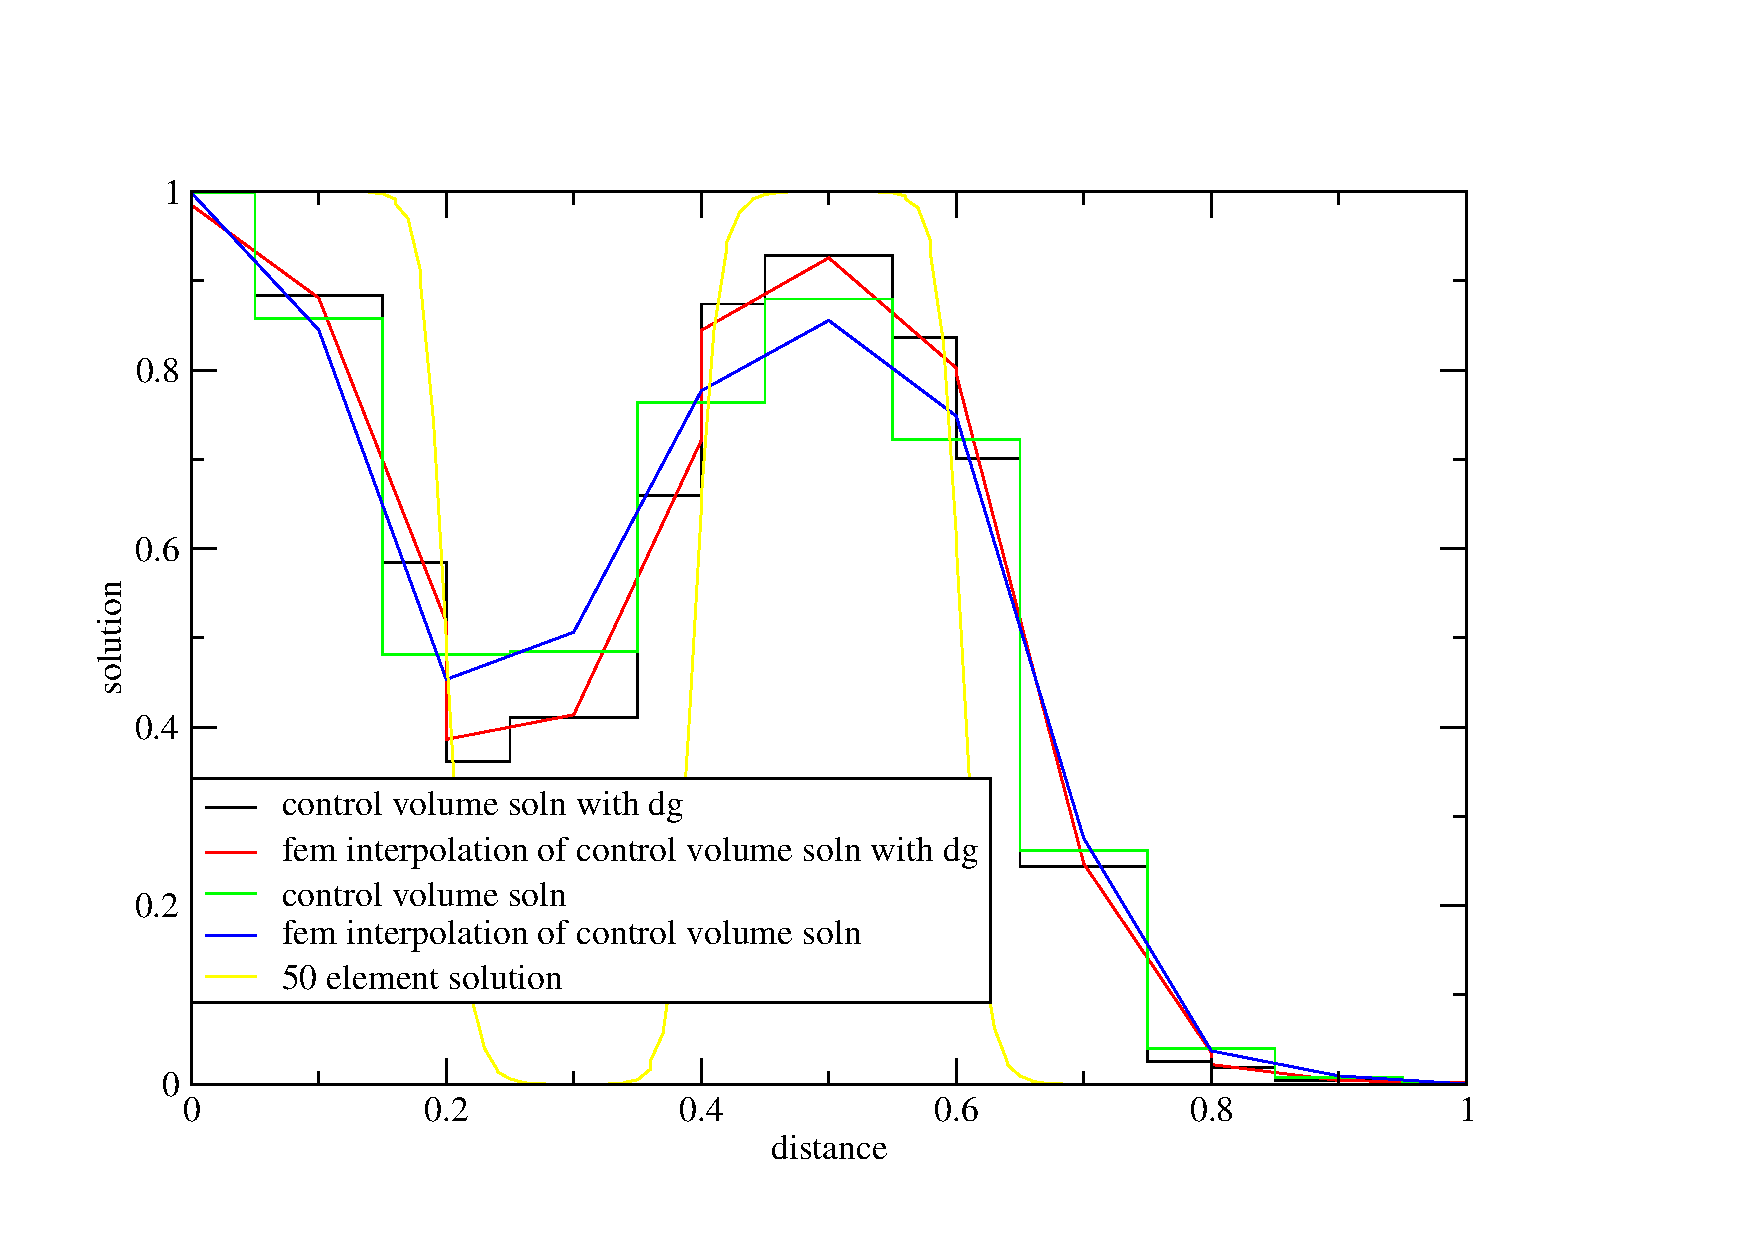
\includegraphics[width=17.5cm,height=12.5cm]{./figures/compar-dg}
\end{center}
\vspace{0.cm}}
\caption{Comparison of discontinuous and continuous (between elements) 
control volume solution for a pure advection problem (from left to right) - 5 finite elements are used and the Courant number (based on the element width of 0.2) 
is 0.005. The solution has been advected a distance of 0.2 with 200 time steps. The 50 element solution is shown to give an indication of the accuracy of the solutions.}
\label{compar-dg}
\end{figure}





\begin{figure}[H]
\vbox{
\begin{center}
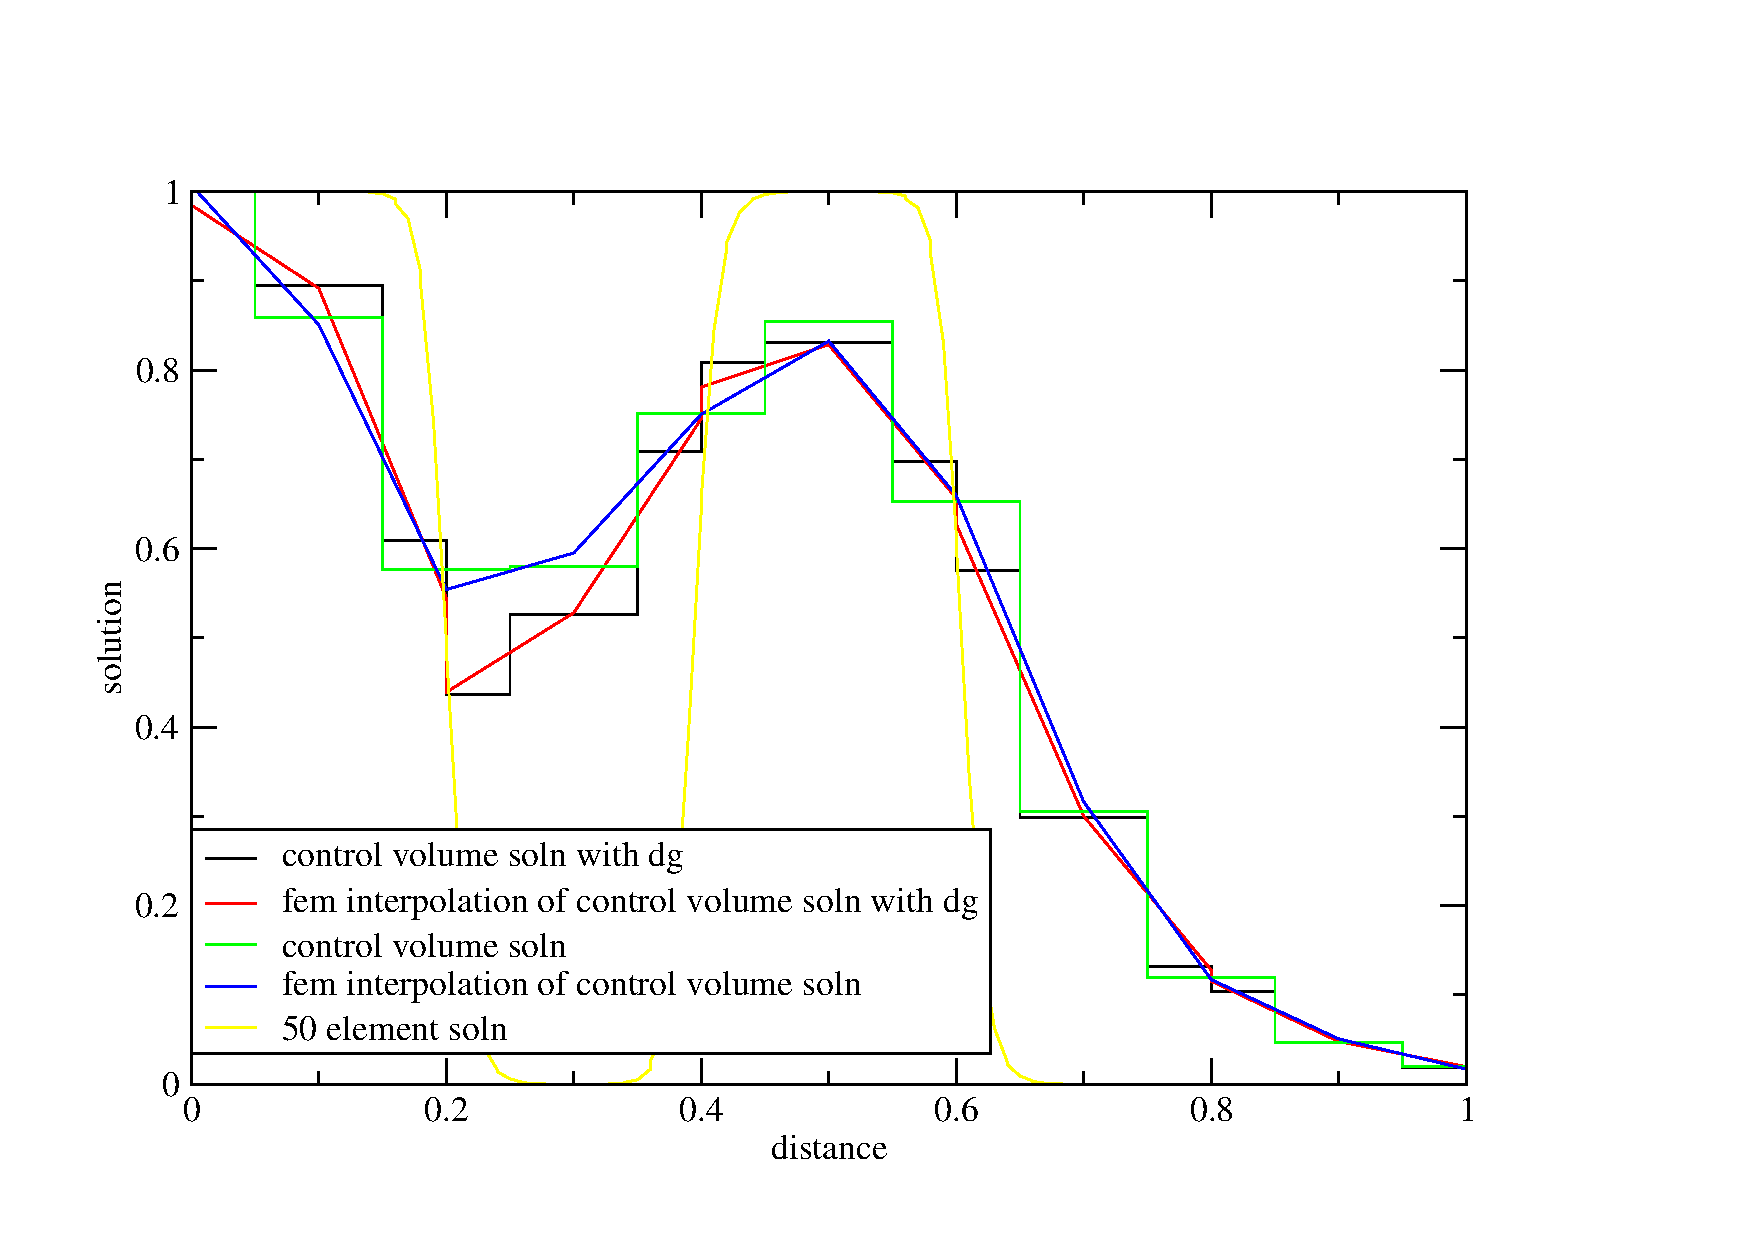
\includegraphics[width=17.5cm,height=12.5cm]{./figures/compar-dg-bdt}
\end{center}
\vspace{0.cm}}
\caption{Comparison of discontinuous and continuous (between elements) 
control volume solution for a pure advection problem (from left to right) - 5 finite elements are used and the Courant number (based on the element width of 0.2) 
is 0.5 (2 based on the minimum width of a control volume). 
The solution has been advected a distance of 0.2 with 2 time steps. The 50 element solution is shown to give an indication of the accuracy of the solutions and has a Courant number (based on the element width) of 0.005. }
\label{compar-dg-bdt}
\end{figure}



\begin{figure}[H]
\vbox{
\begin{center}
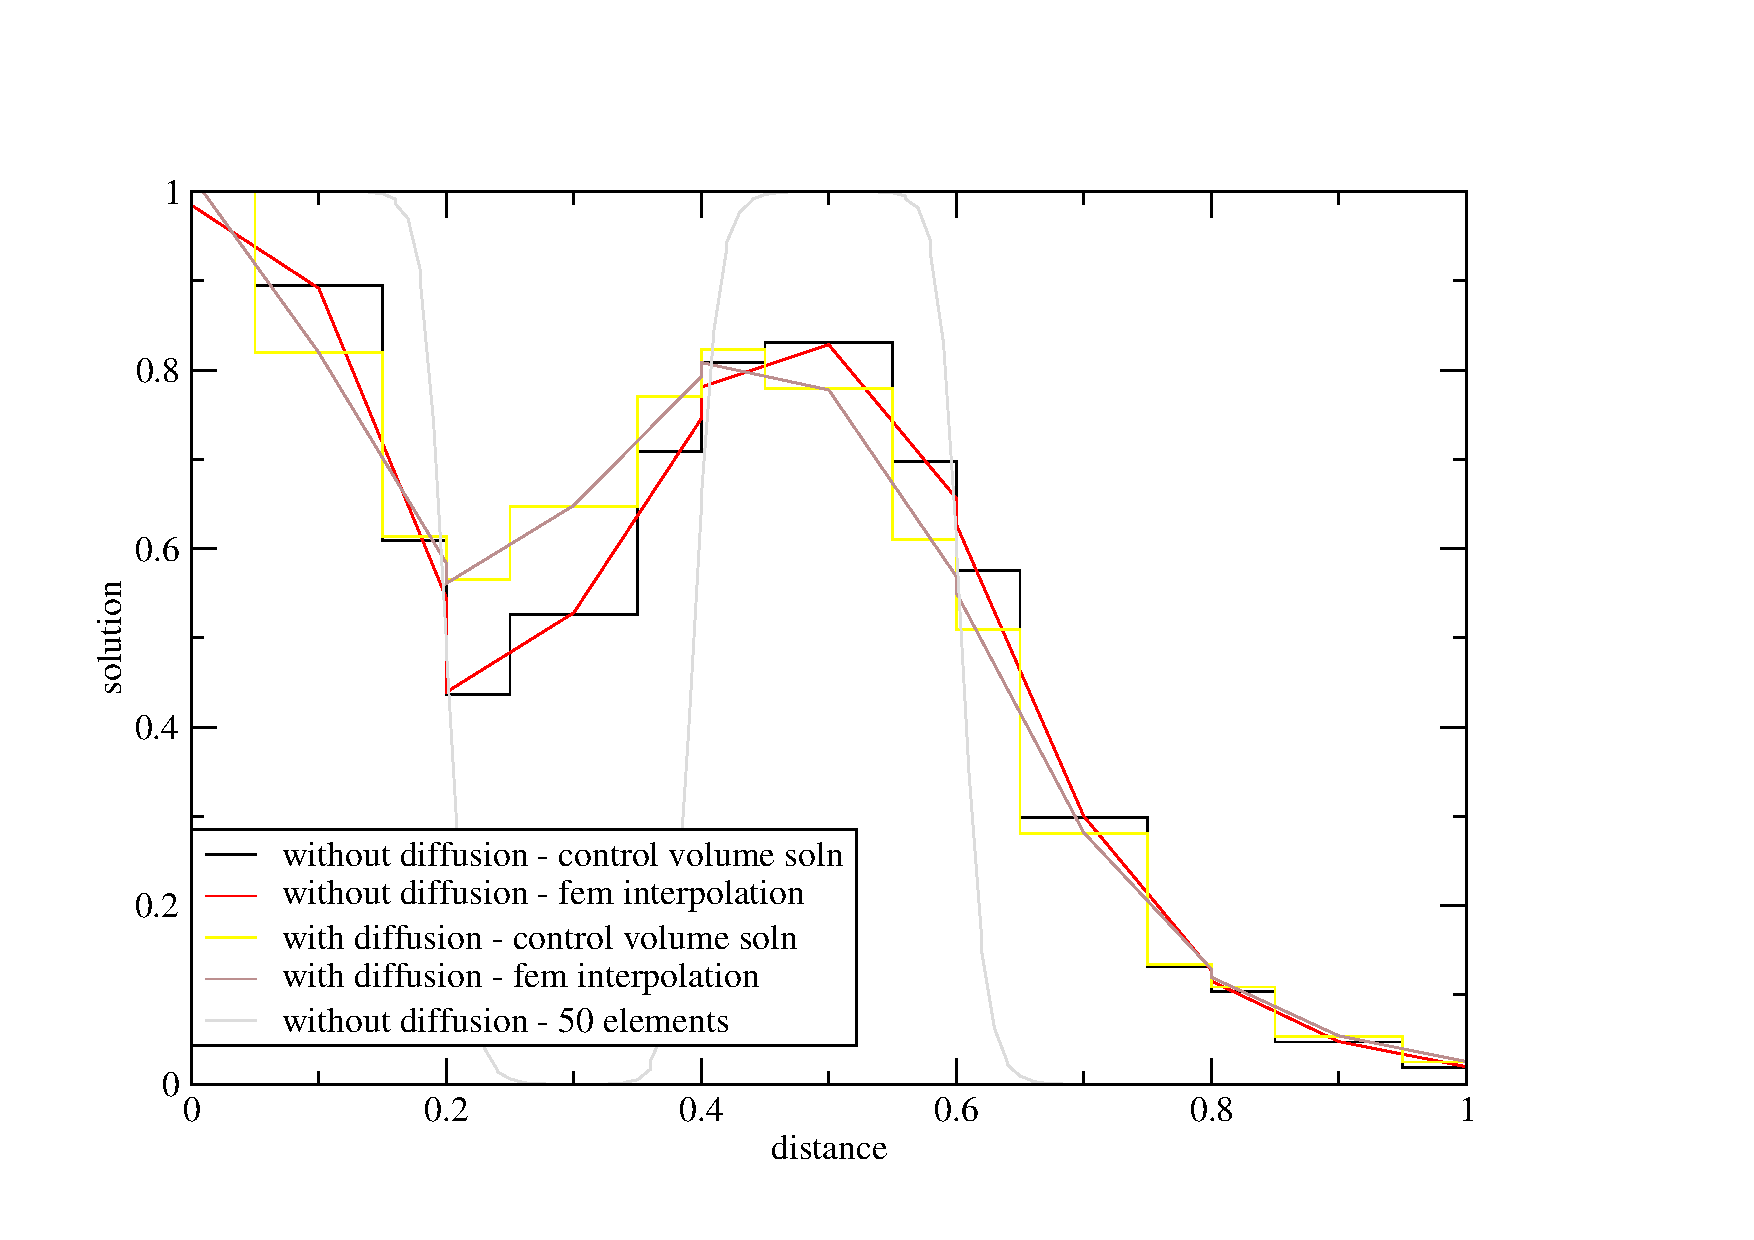
\includegraphics[width=17.5cm,height=12.5cm]{./figures/compar-dg-bdt-diff}
\end{center}
\vspace{0.cm}}
\caption{The effect of diffusion using a discontinuous (between elements) 
control volume solution for an advection problem (from left to right) - 5 finite elements are used and the Courant number (based on the element width of 0.2) 
is 0.5 (2 based on the minimum width of a control volume). 
The solution has been advected a distance of 0.2 with 2 time steps. The 50 element solution is for pure advection and is shown to give an indication of the accuracy of the solutions and has a Courant number (based on the element width) of 0.005. }
\label{compar-dg-bdt-diff}
\end{figure}




\begin{figure}[H]
\vbox{
\begin{center}
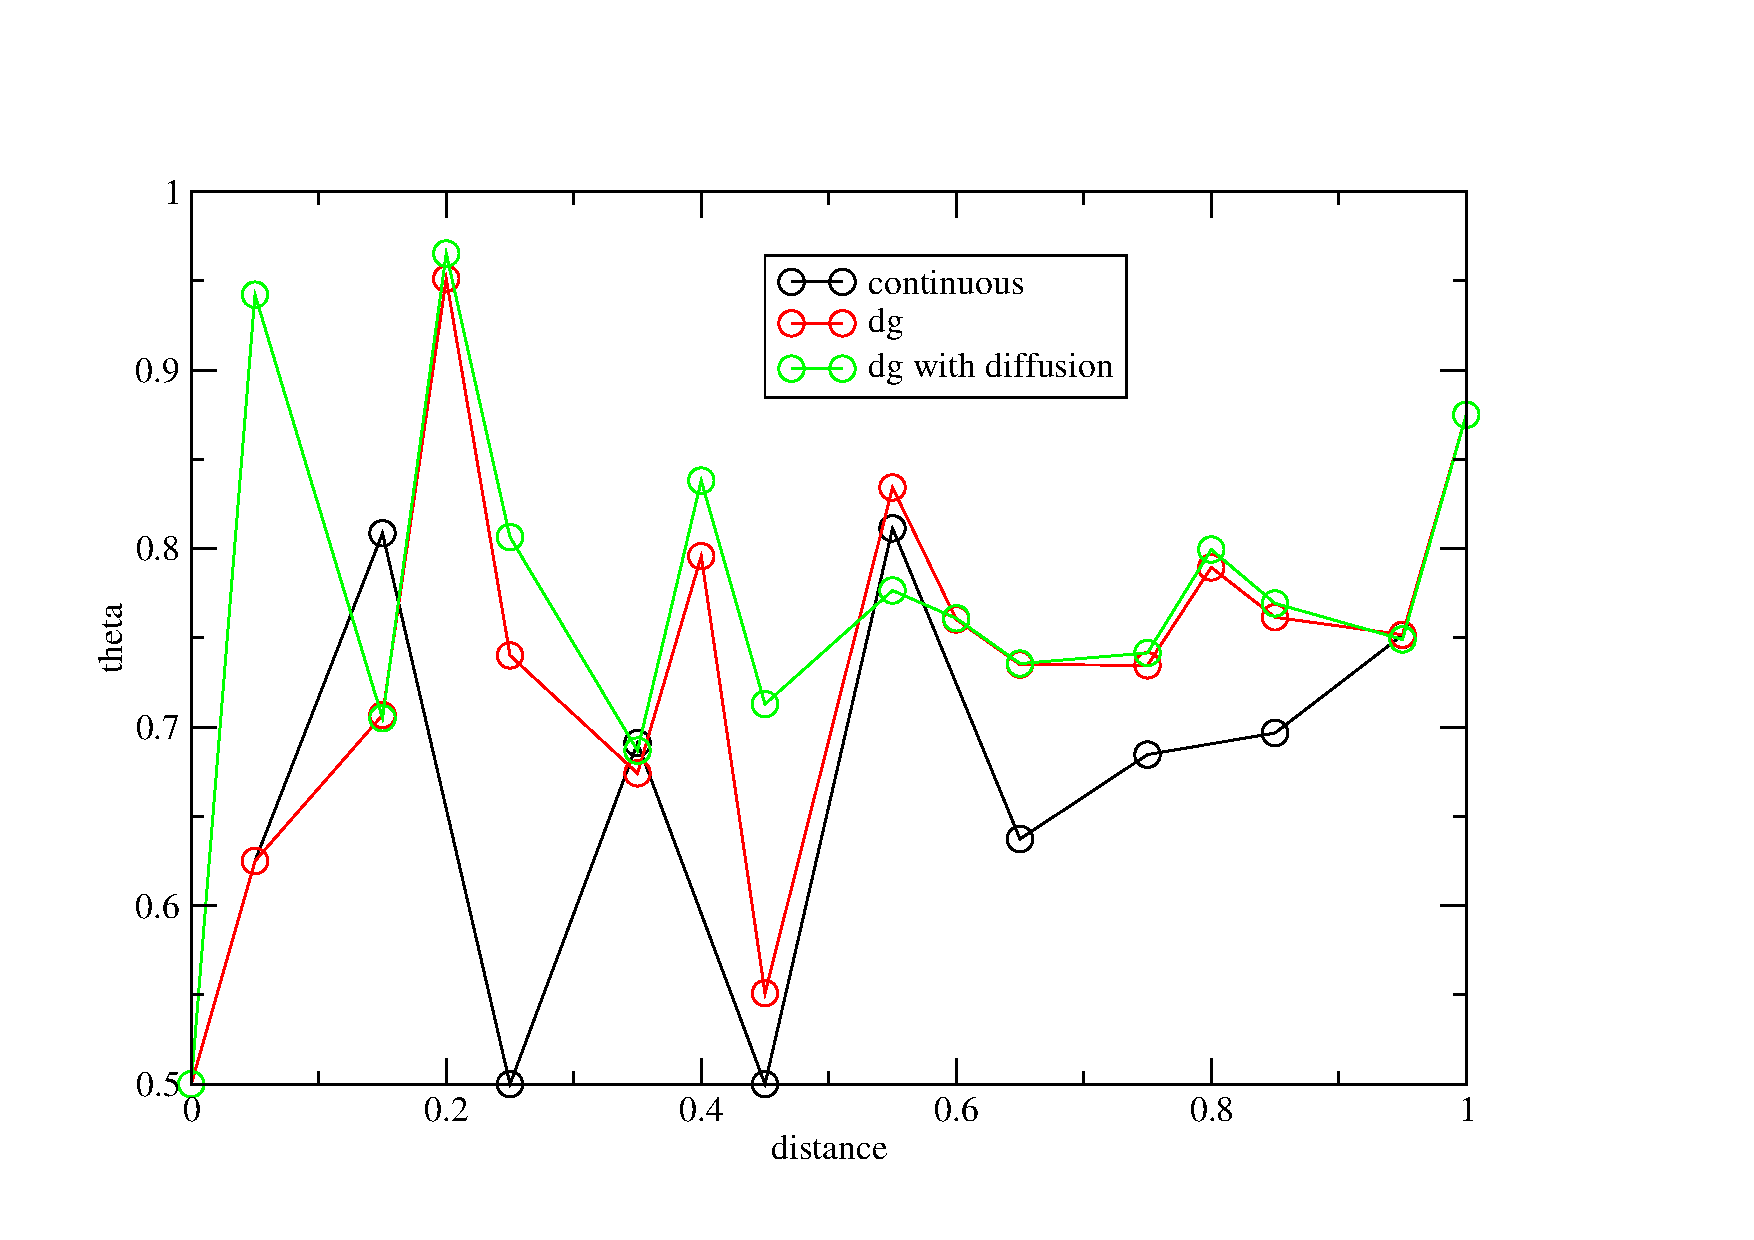
\includegraphics[width=17.5cm,height=12.5cm]{./figures/theta-bdt}
\end{center}
\vspace{0.cm}}
\caption{Value of the $\theta$ 'theta' time stepping parameter on the faces of the control volumes at the end of the 
simulation  - 5 finite elements are used and the Courant number (based on the element width of 0.2) 
is 0.5 (2 based on the minimum width of a control volume). 
The solution has been advected a distance of 0.2 with 2 time steps.  }
\label{theta-bdt}
\end{figure}


\begin{figure}[H]
\vbox{
\hbox{
\hspace{-1.cm}
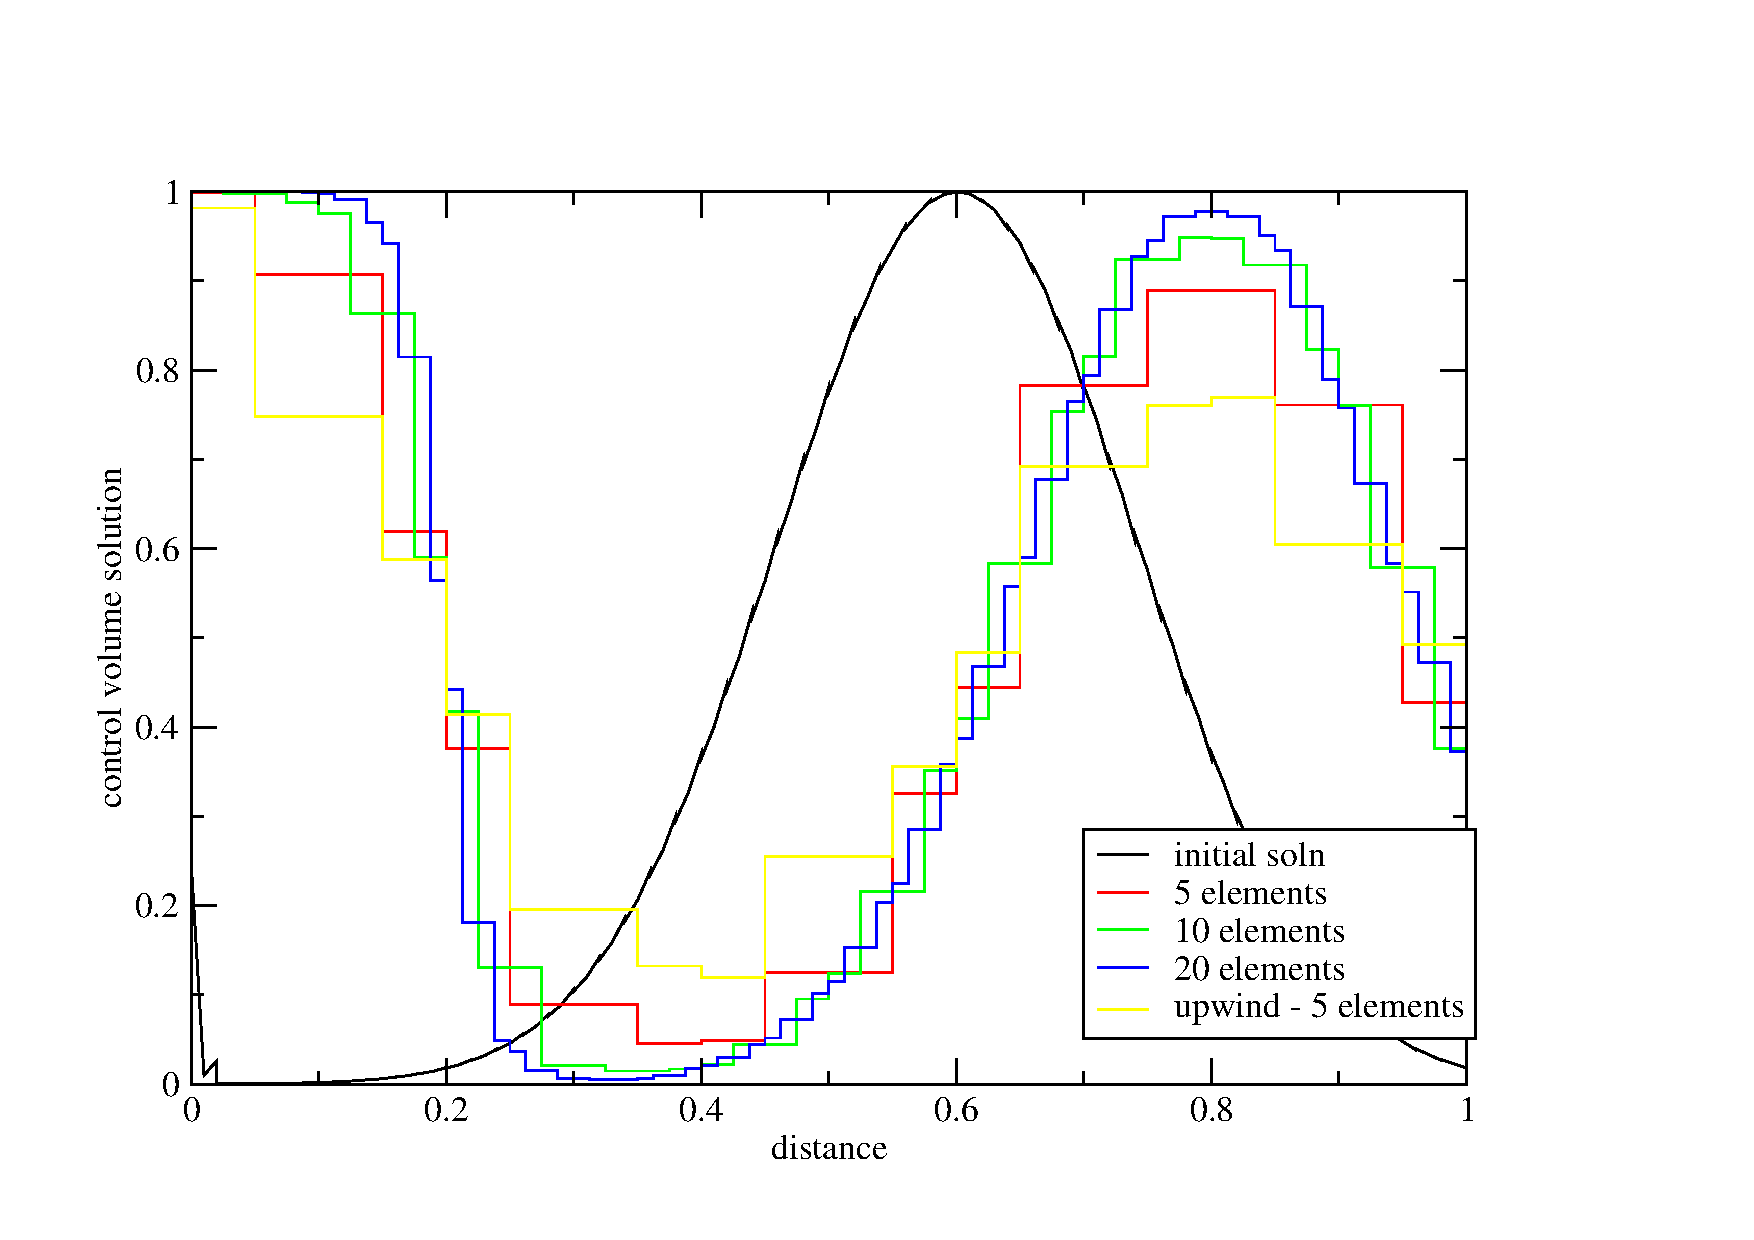
\includegraphics[width=9.0cm,height=9.cm]{./figures/converg-cv}
\hspace{-1.cm}
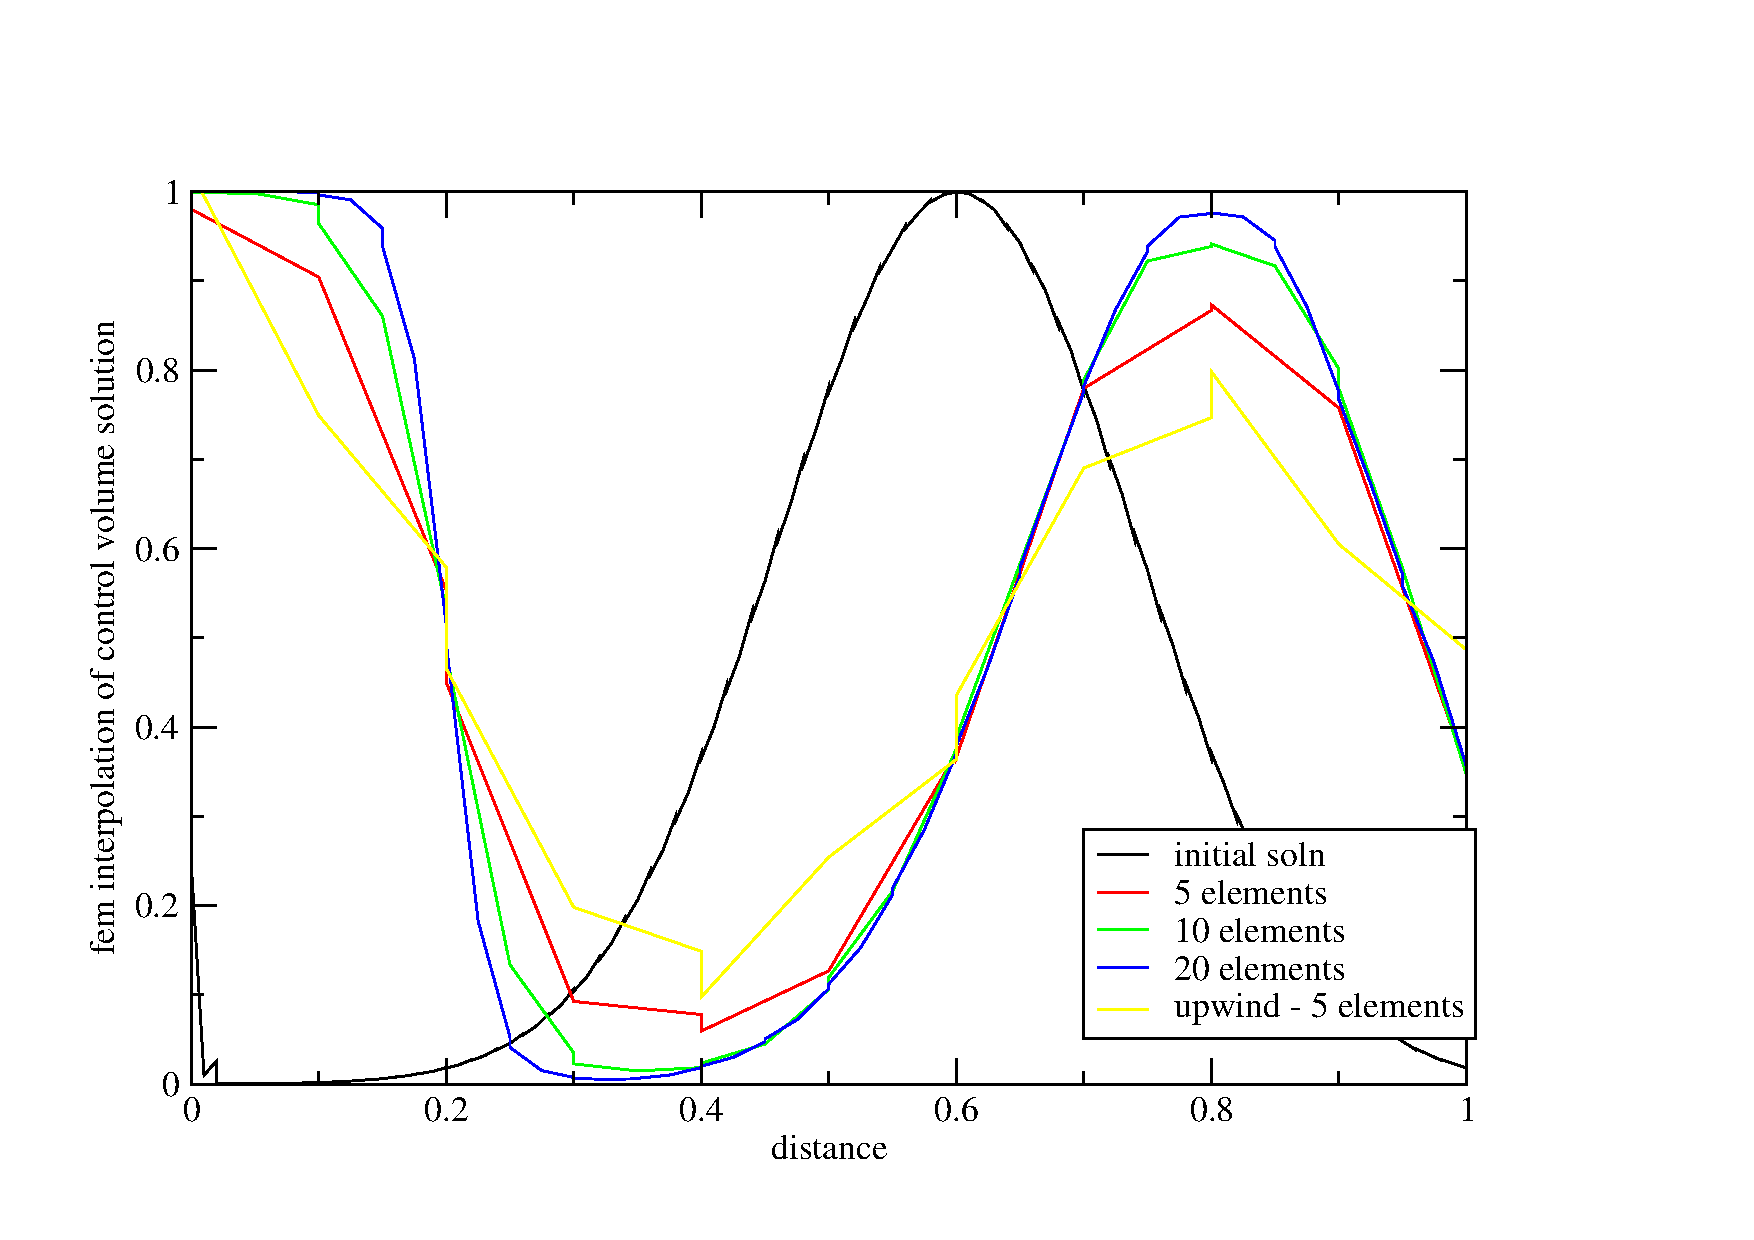
\includegraphics[width=9.0cm,height=9.cm]{./figures/converg-fem}
}
\vspace{-0.cm}
\hbox{\hspace{4.cm}(a) \hspace{6.5cm}(b)}
\vspace{-0.cm}}
\label{converg}
\caption{Convergence of the solutions with discontinuity between elements and with increased resolution. A pure advection problem (from left to right) - the Courant number  
is 0.005. The solution has been advected a distance of 0.2. (a) the control volume solutions are shown. (b) the FEM interpolation of the control volume solutions are shown. }
\end{figure}


\begin{figure}[H]
\vbox{
\begin{center}
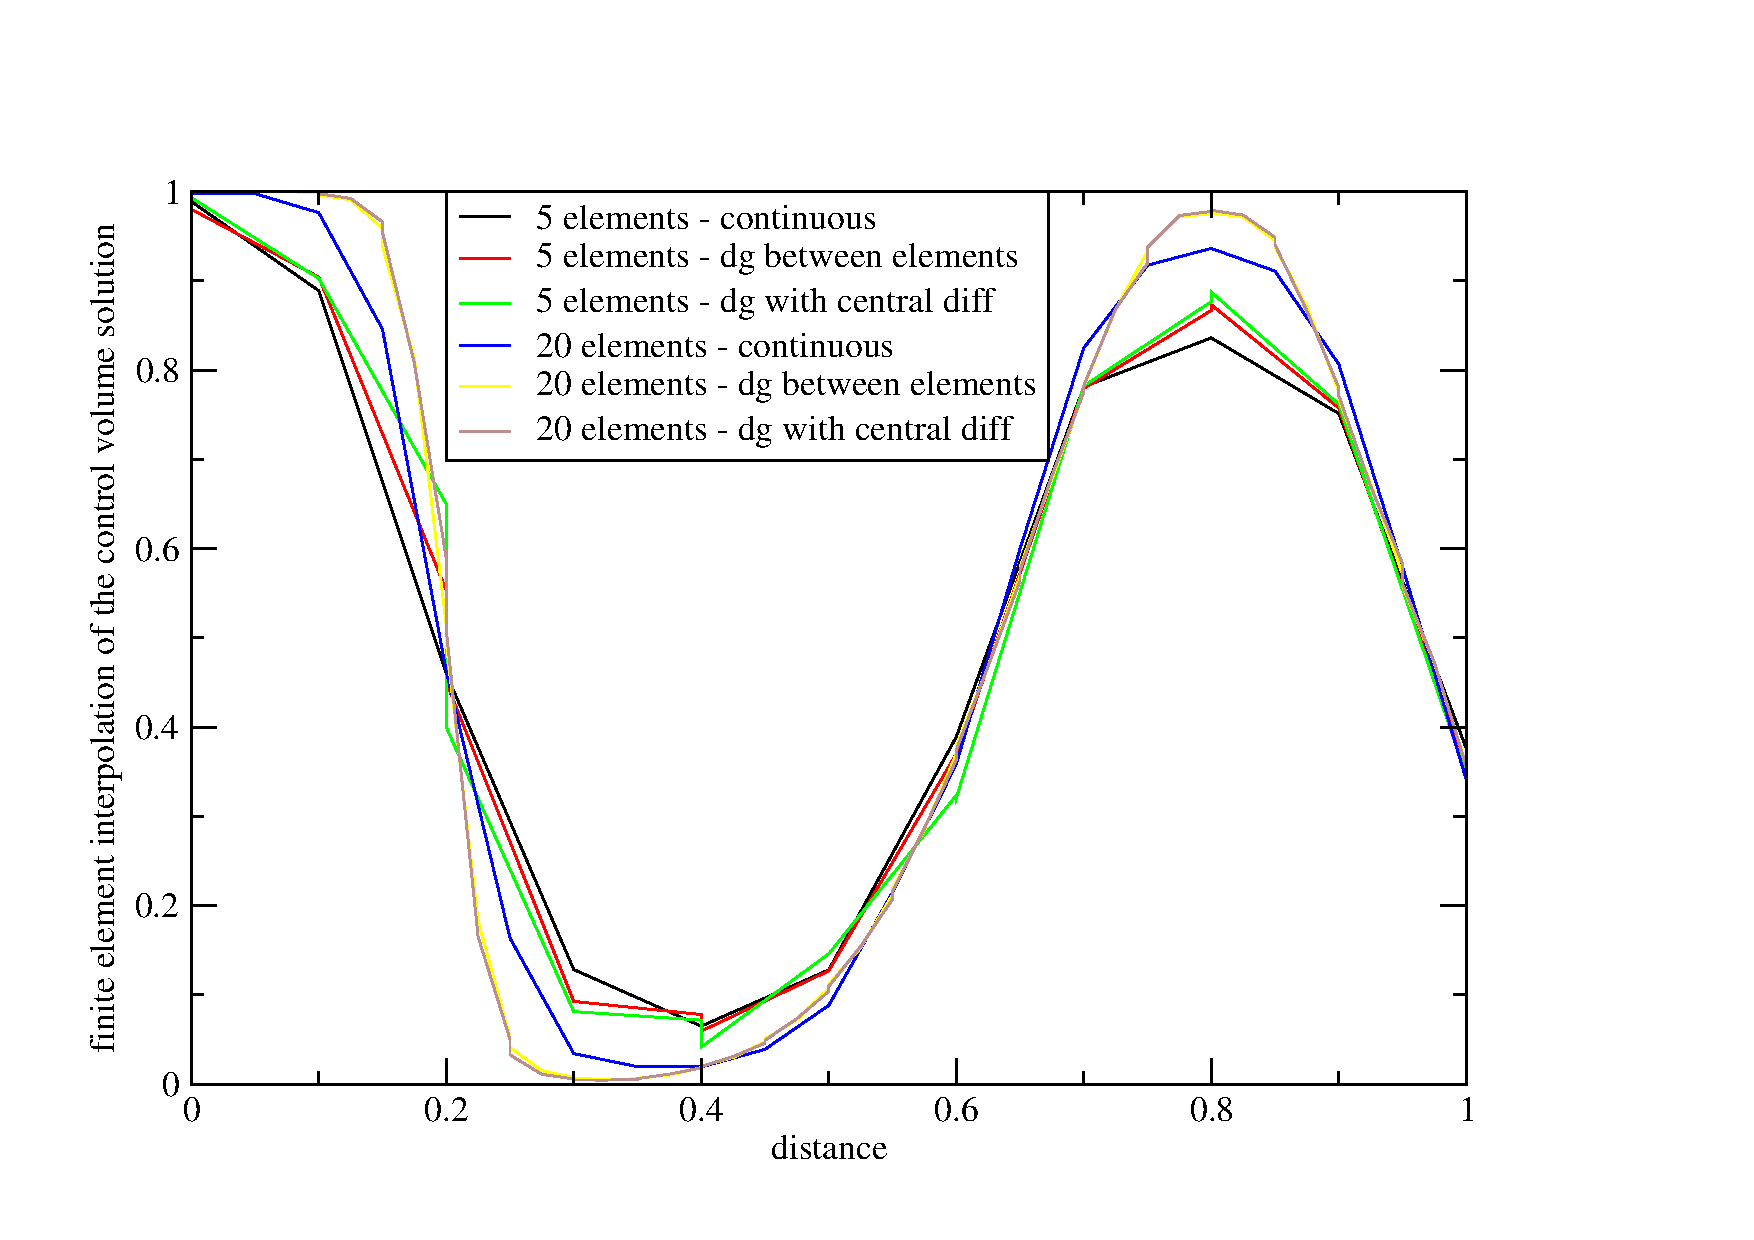
\includegraphics[width=17.5cm,height=12.5cm]{./figures/converg-compare-fem}
\end{center}
\vspace{0.cm}}
\caption{Comparison of convergence of the solutions with and without discontinuity between elements and with an upwind and central difference flux between the elements and with increased resolution. A pure advection problem (from left to right) - the Courant number  
is 0.005. The solution has been advected a distance of 0.2. The FEM interpolation of the control volume solutions are shown.  }
\label{converg-compare-fem}
\end{figure}


